\newpage
\section{Plots}
\label{sec:Plots}

Here is a section of common plots that were produced with the GeanePlots module. (This is not all-inclusive.) These plots were generated with the makeGEANEPlots.fcl file with version v7\_06\_01 for truthLRFit tracks. (Plots for the other fit modes are not included in this section. There are more poorly fitted tracks or wider distributions accordingly. One can see the various DocDBs referenced in this document in order to see what those fits look like, or generate those fits directly.) There is no plane number cut in these plots, but there is a truth energy cut of 3 MeV to cut out some poor events. The tracks these plots describe were generated starting with 7000 muons times 500 grid jobs, 3.5 M muons, with the mdc1.fcl file, resulting in approximately 140,000 tracks. All three trackers were included in the simulation, unnecessary geometry was omitted (such as calorimeters), the trajectory art records were not recorded, orphans were not tracked, and normal material was included. If checking out this documentations repository, then the analyzer root file is located in ``Images/MainPlots/gm2GEANE\_ana\_19831354\_1504040981.139.root''.

Branch and commit numbers used to generate these plots are listed below: \\

artg4 - feature/trackDevelop - ed5436 \\

gm2analyses - develop - b470cb7 \\

gm2dataproducts - feature/trackDevelop - 4fb1dc \\

gm2geom - feature/trackDevelop - c623aa9 \\

gm2ringsim - feature/trackDevelop - 9684d18 \\

gm2tracker - feature/trackDevelop - aa9239e \\

gm2util - feature/trackDevelop - 17b7856 \\

The sam-data-set names are ``nkinnaird\_documentation\_events\_mdc1\_reduced'' and \\
``nkinnaird\_documentation\_tracks\_truthLRFit'' for the events and tracks respectively.
Some more information including the locations of the sam-data-sets and root files are included in the directory: \\
``/pnfs/GM2/persistent/Tracking/nkinnaird/Documentation''

\begin{figure}
    \centering
    \begin{subfigure}[]{0.7\textwidth}
        \centering
        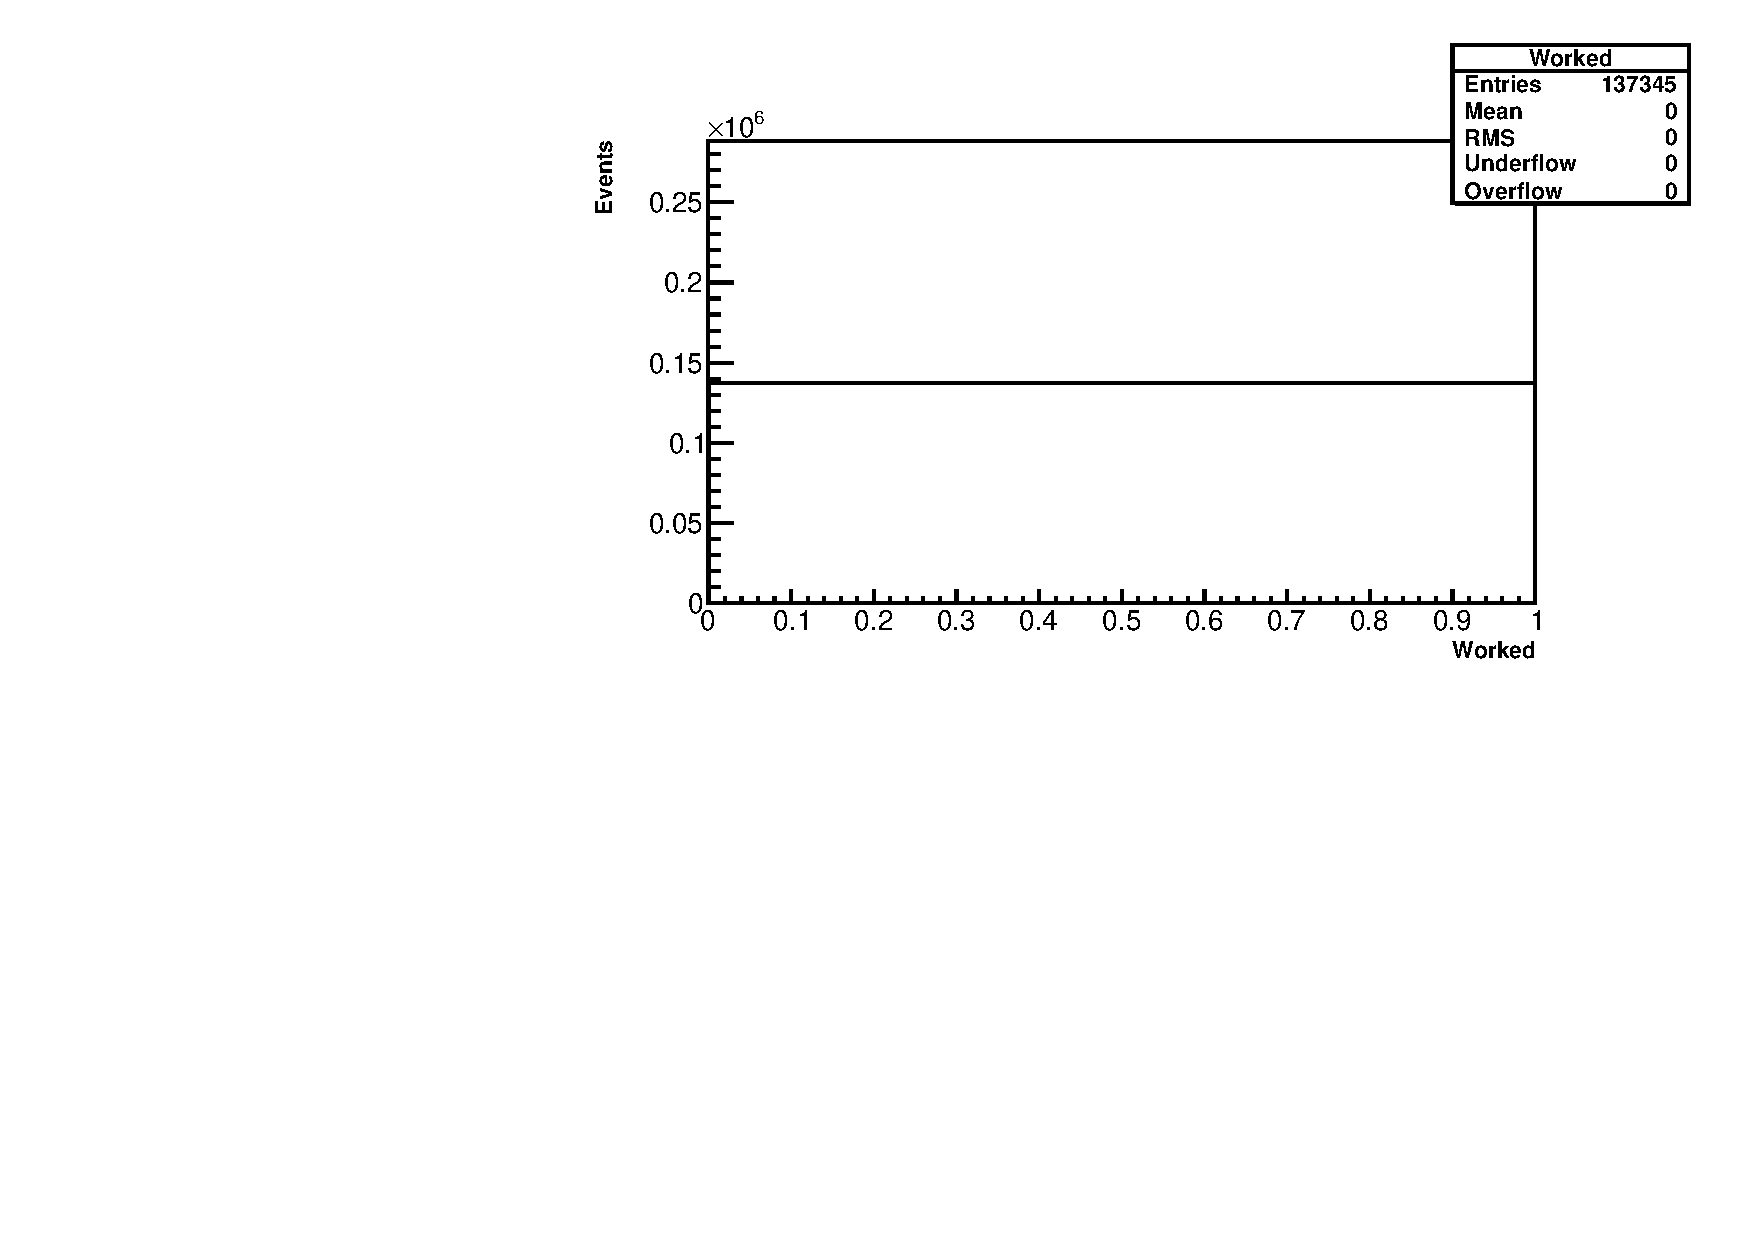
\includegraphics[width=1\textwidth]{WorkedEvents} 
        \caption{Number of events that passed the track fitting, with no cuts applied.}
        \label{fig:worked}
    \end{subfigure}
    
    \begin{subfigure}[]{0.7\textwidth}
        \centering
        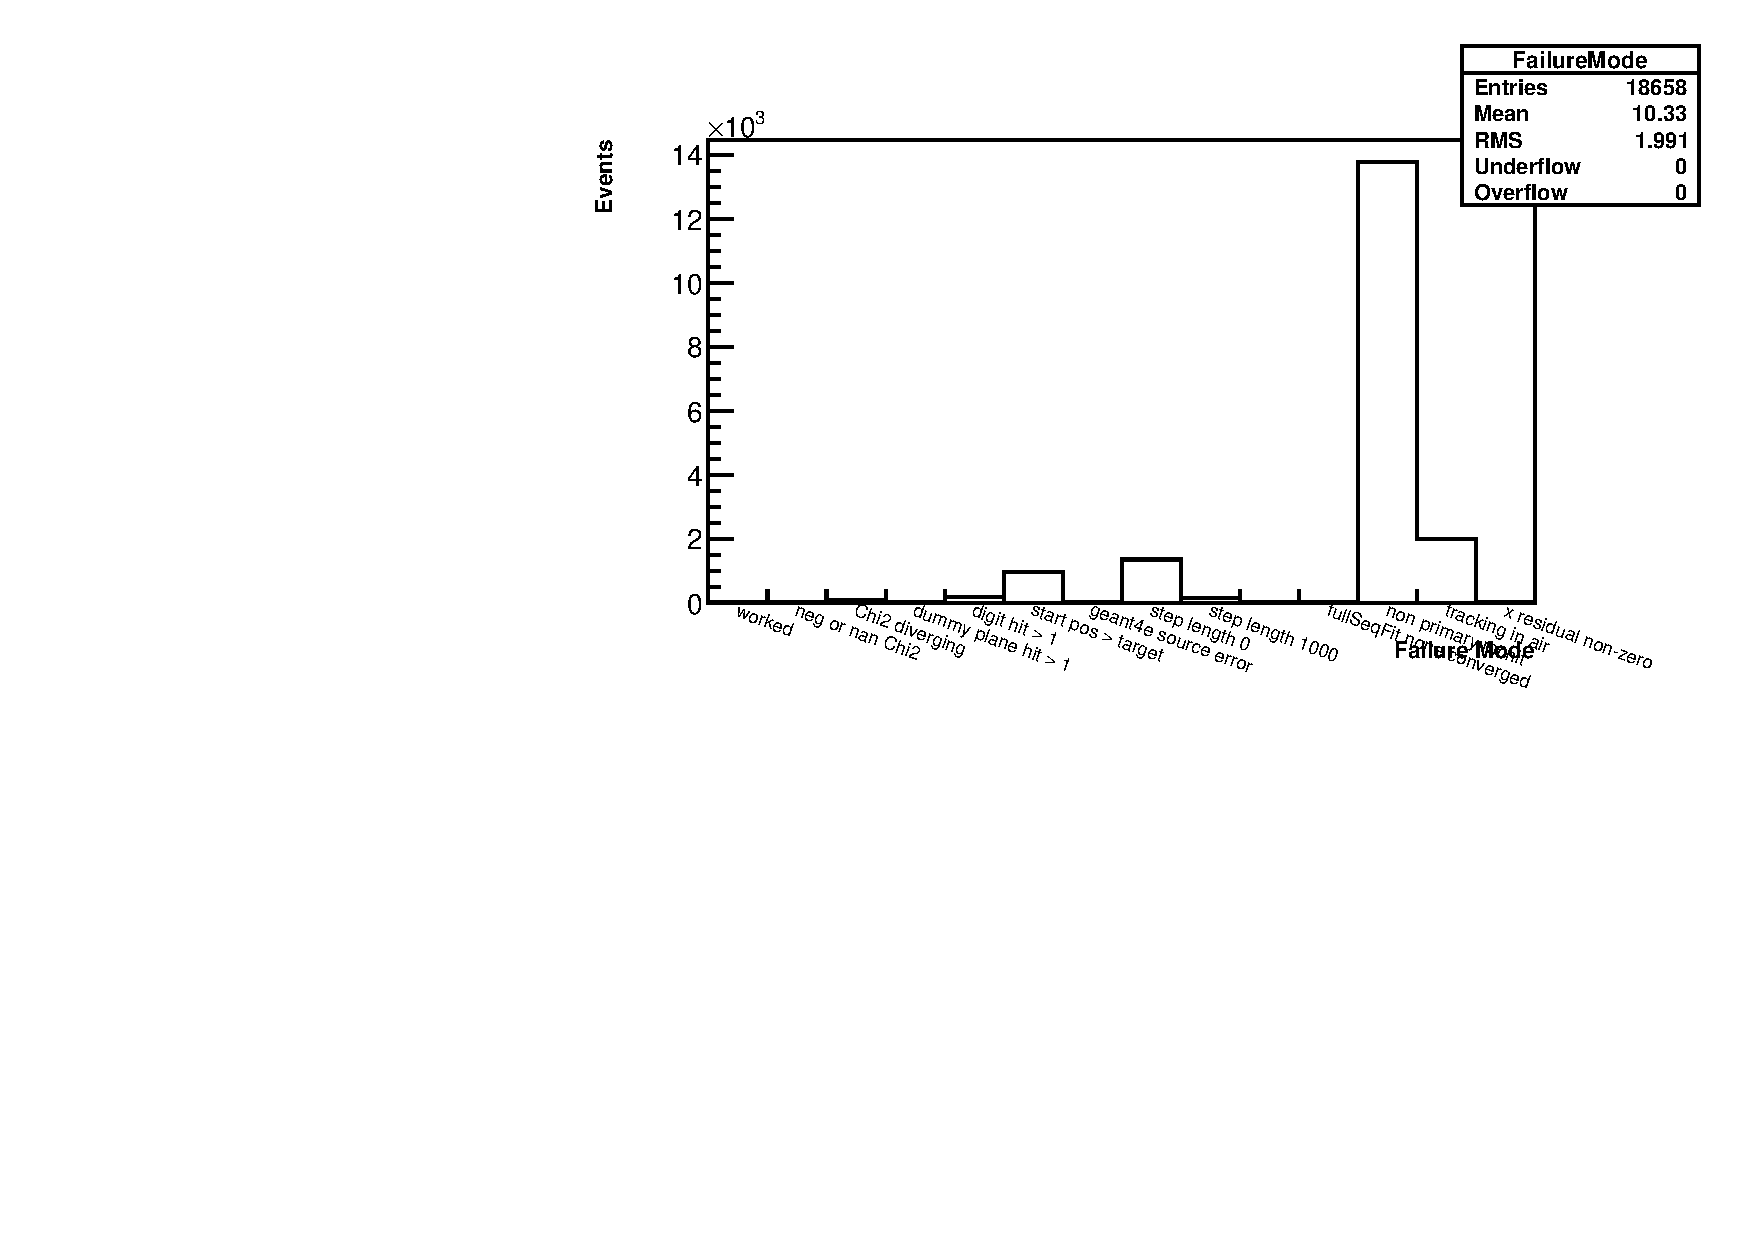
\includegraphics[width=1\textwidth]{FailedEventsUnzoomed} 
        \caption{Failure modes for the track reconstruction. Most ``failures'' are Geant issues.}
    \end{subfigure}

    \begin{subfigure}[]{0.7\textwidth}
        \centering
        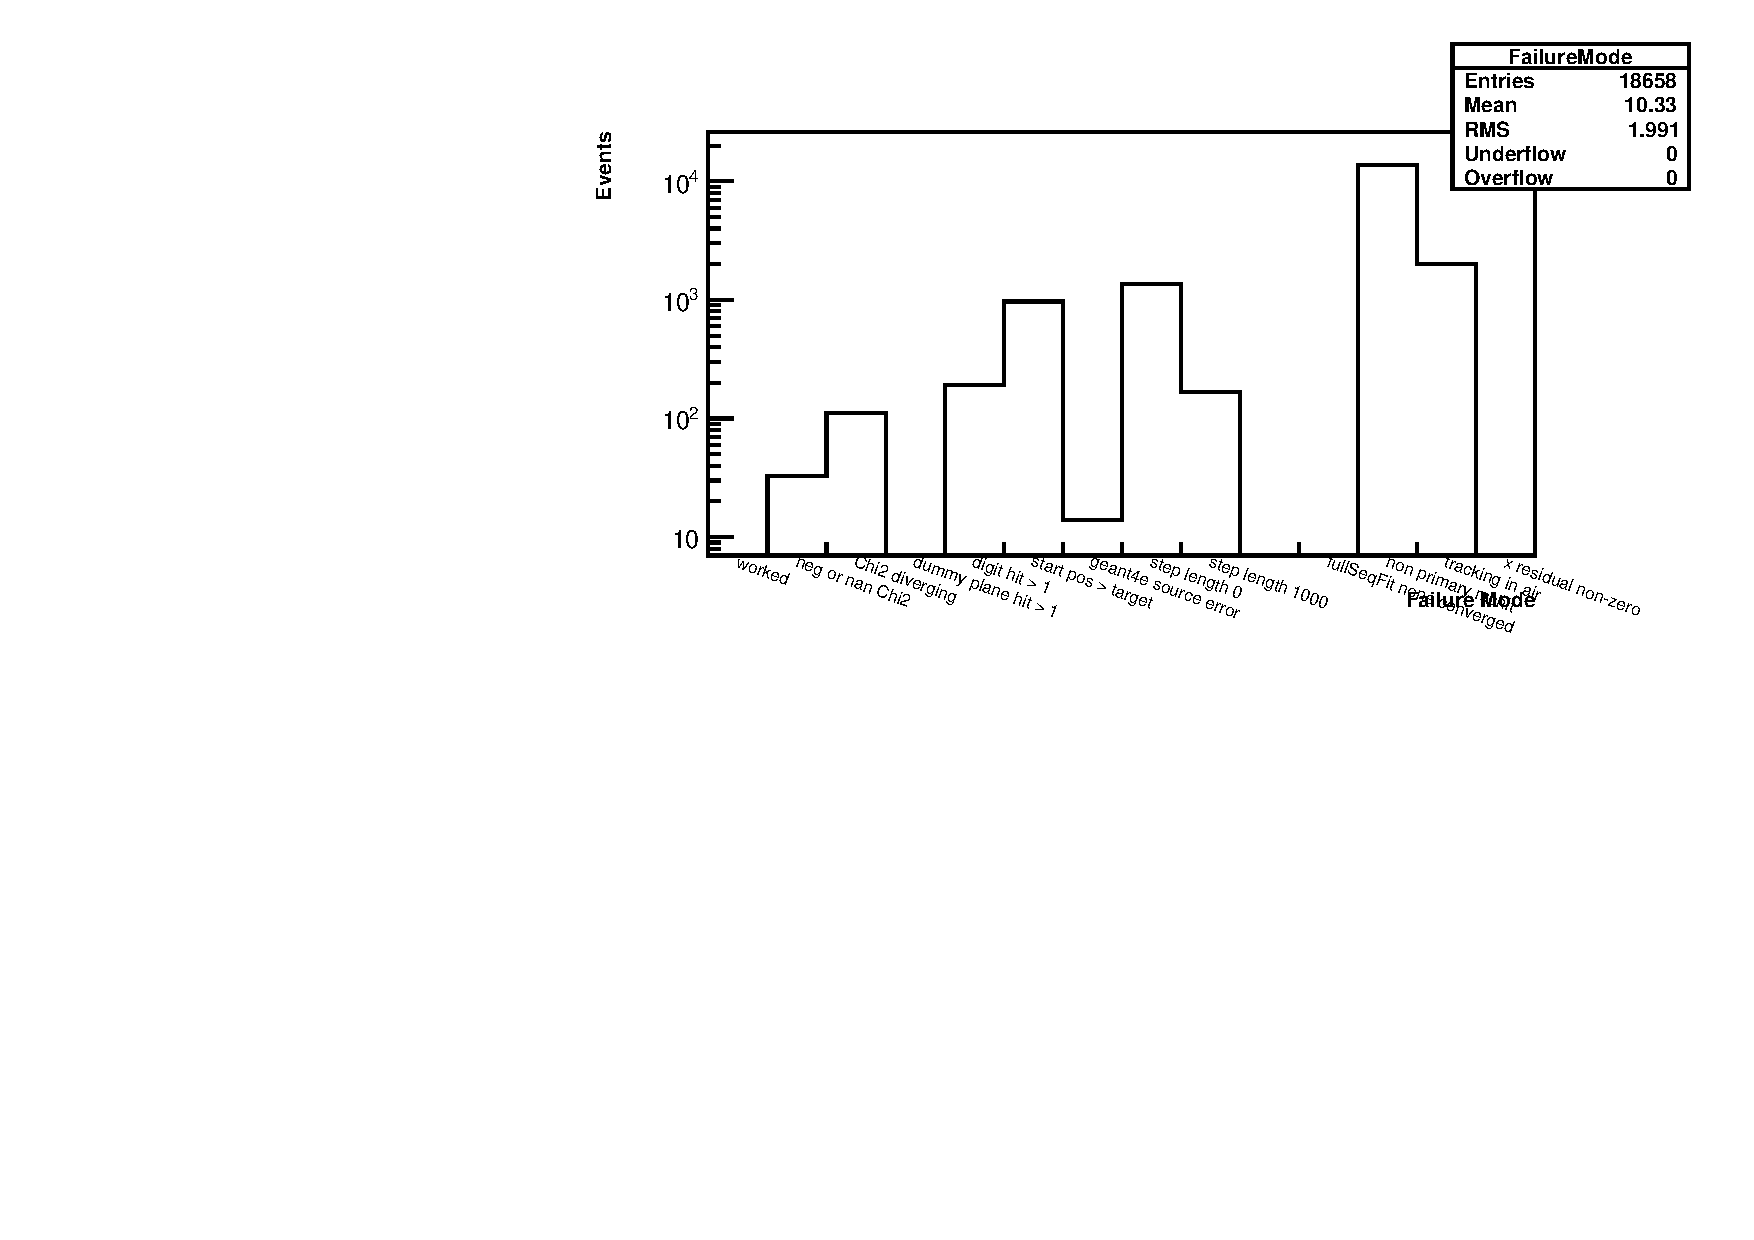
\includegraphics[width=1\textwidth]{FailedEventsLog} 
        \caption{Log plot of the failure modes. The first two failure mode bins are the most important.}
    \end{subfigure}

    \caption{The number of events that passed and failed the Geane track fitting.}
\end{figure}



\begin{figure}
    \centering
    \begin{subfigure}[]{0.7\textwidth}
        \centering
        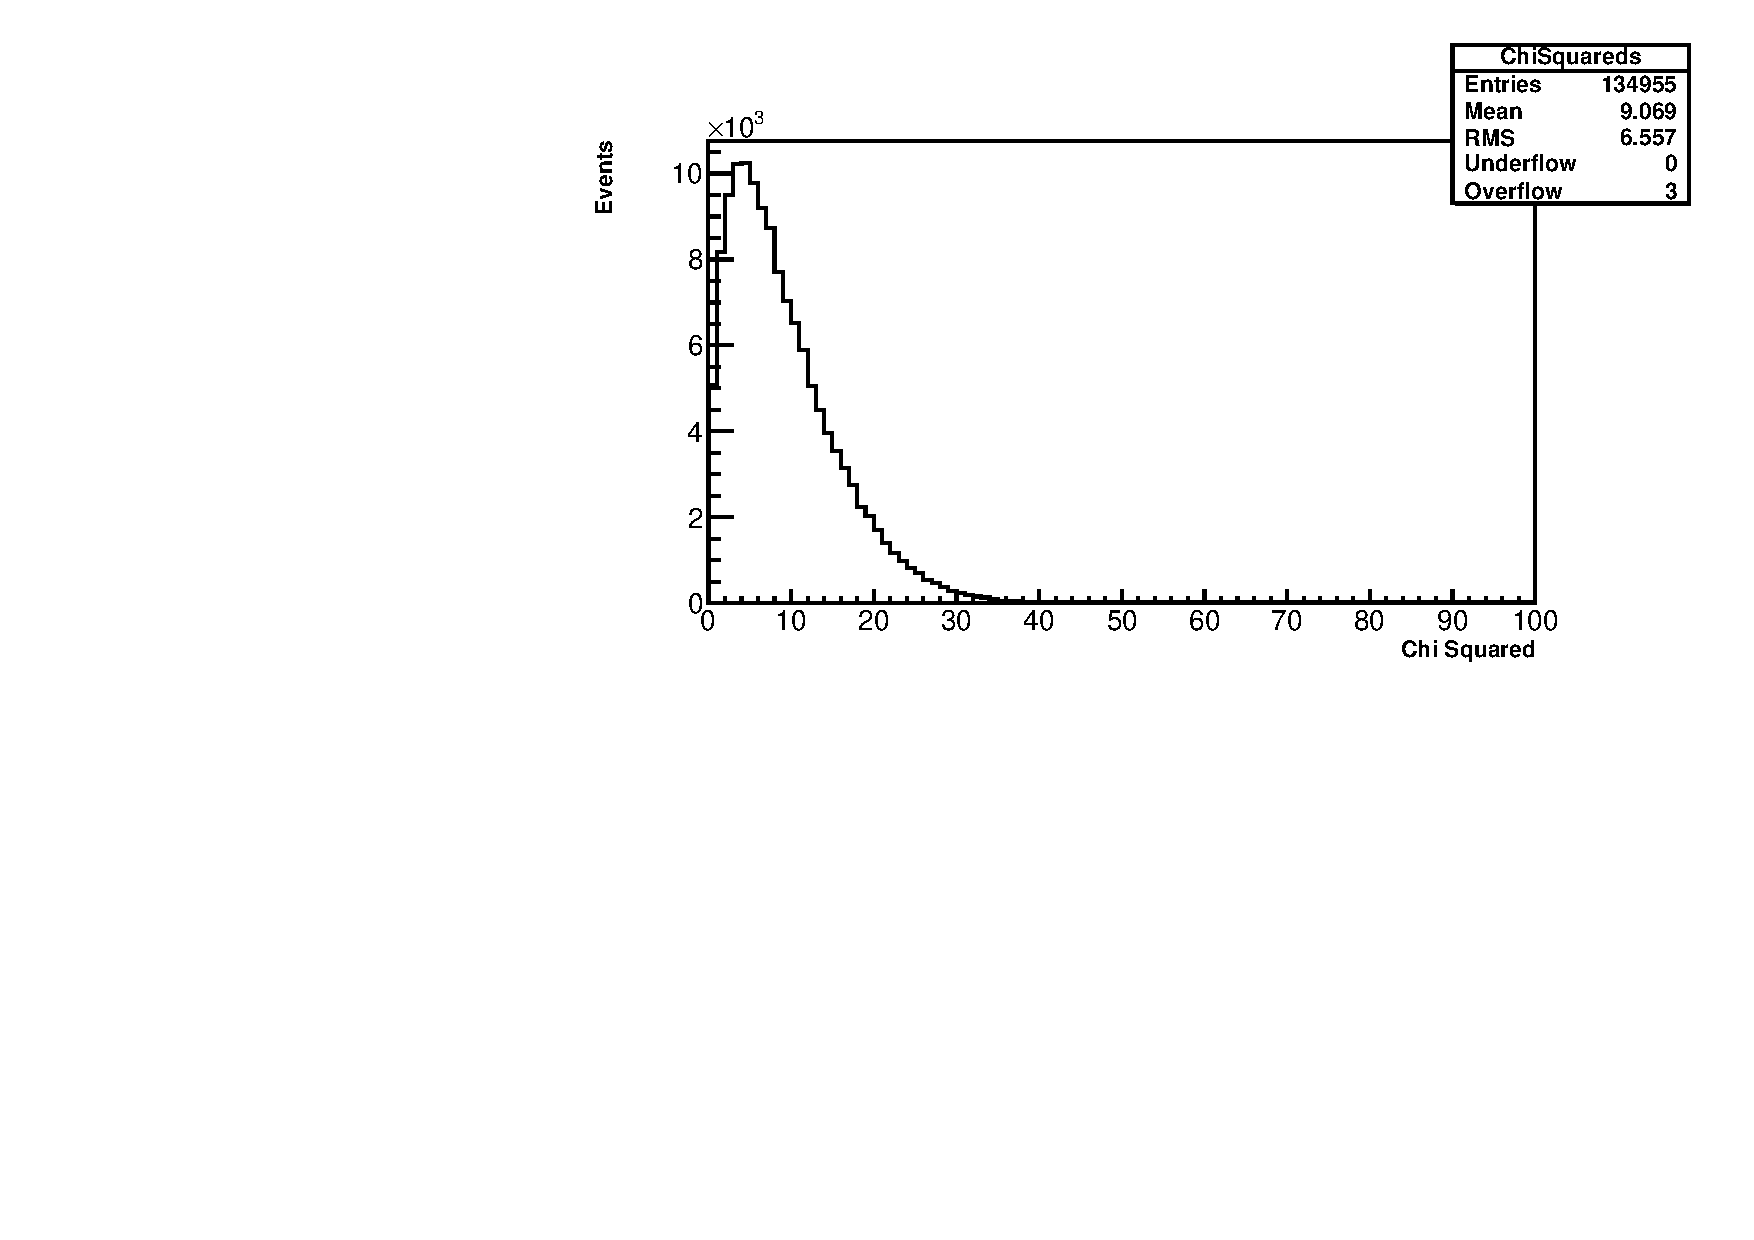
\includegraphics[width=1\textwidth]{chi2} 
        \caption{Distribution of $\chi^{2}$s for all tracks. Comprised of separate $\chi^{2}$ distributions with degrees of freedom equal to the number of planes hit minus 5.}
    \end{subfigure}
    
    \begin{subfigure}[]{0.7\textwidth}
        \centering
        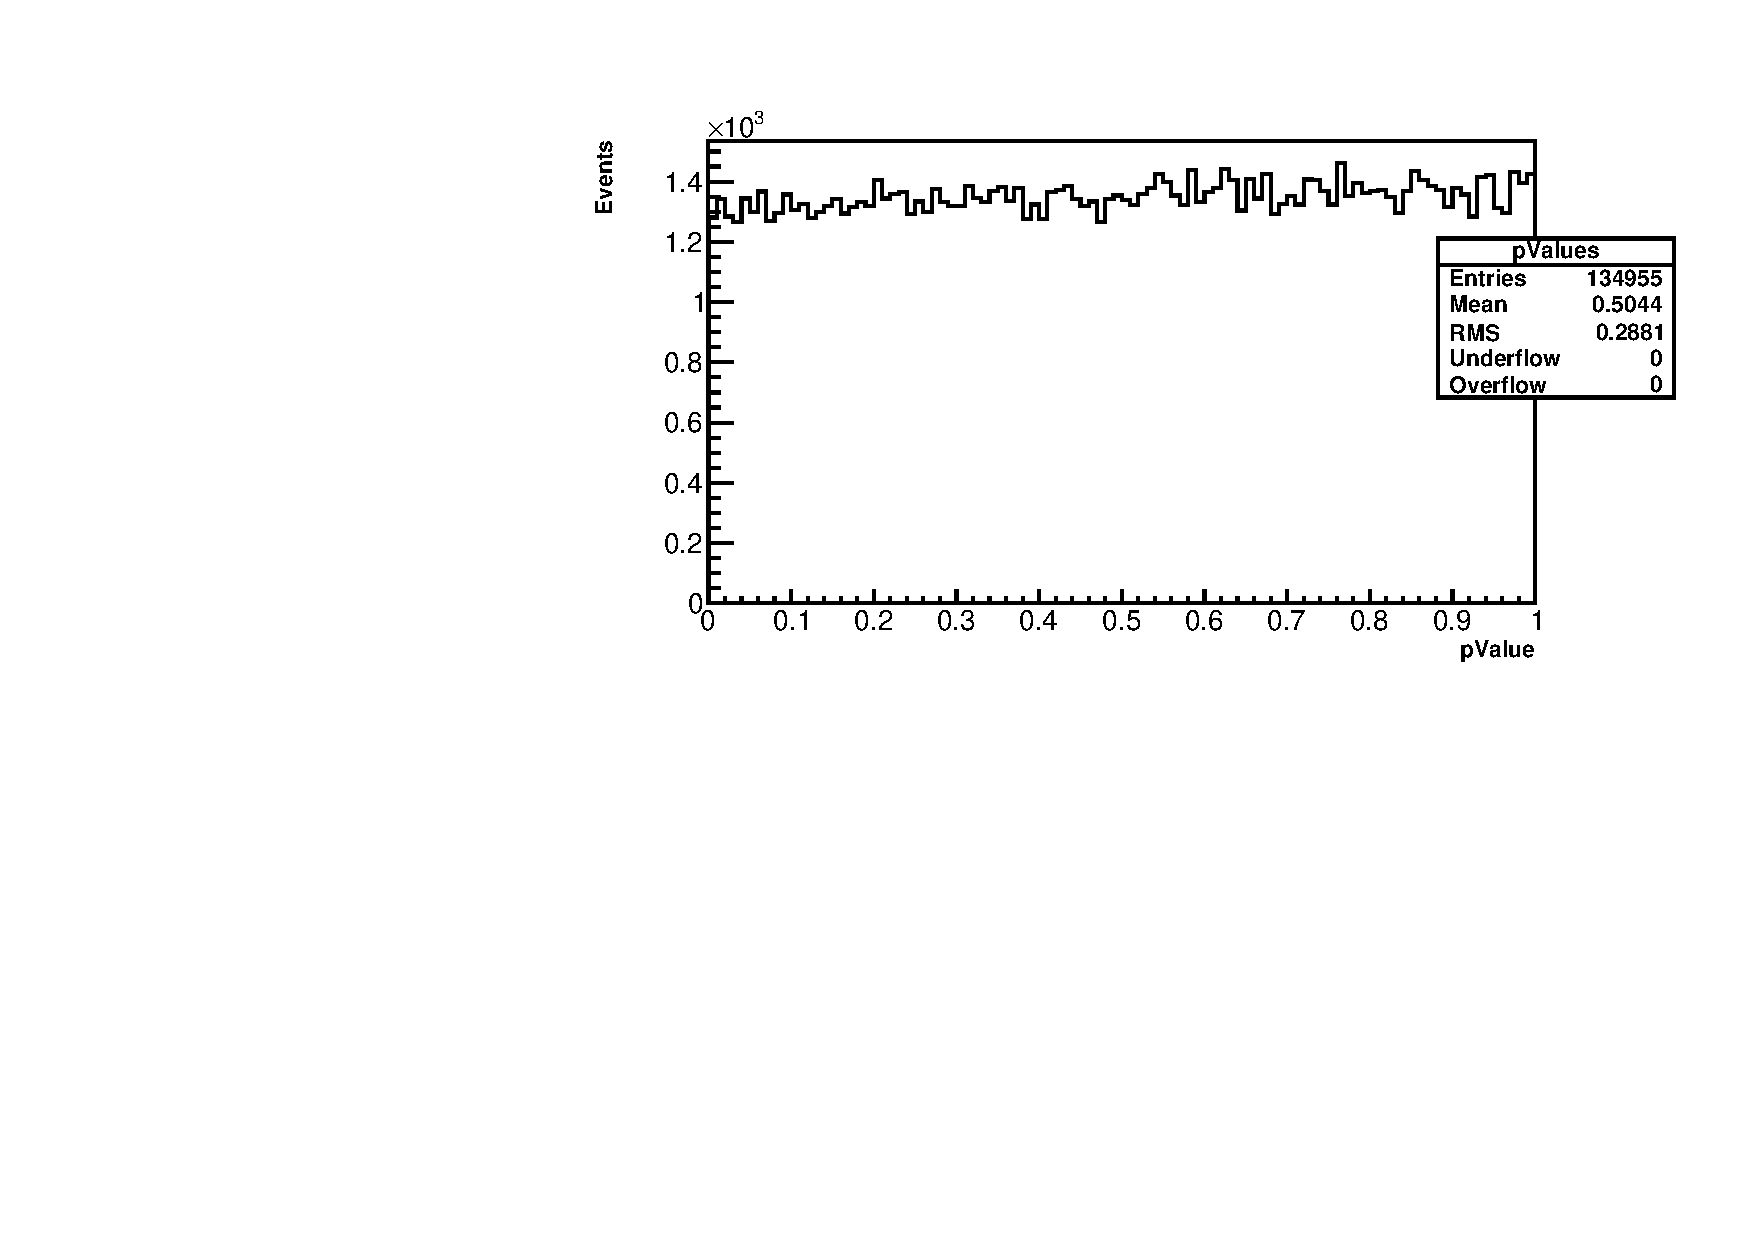
\includegraphics[width=1\textwidth]{pValueUnzoomed} 
        \caption{P-value distribution for tracks. Very nearly uniform, showing tracking is working as expected.}
    \end{subfigure}

    \begin{subfigure}[]{0.7\textwidth}
        \centering
        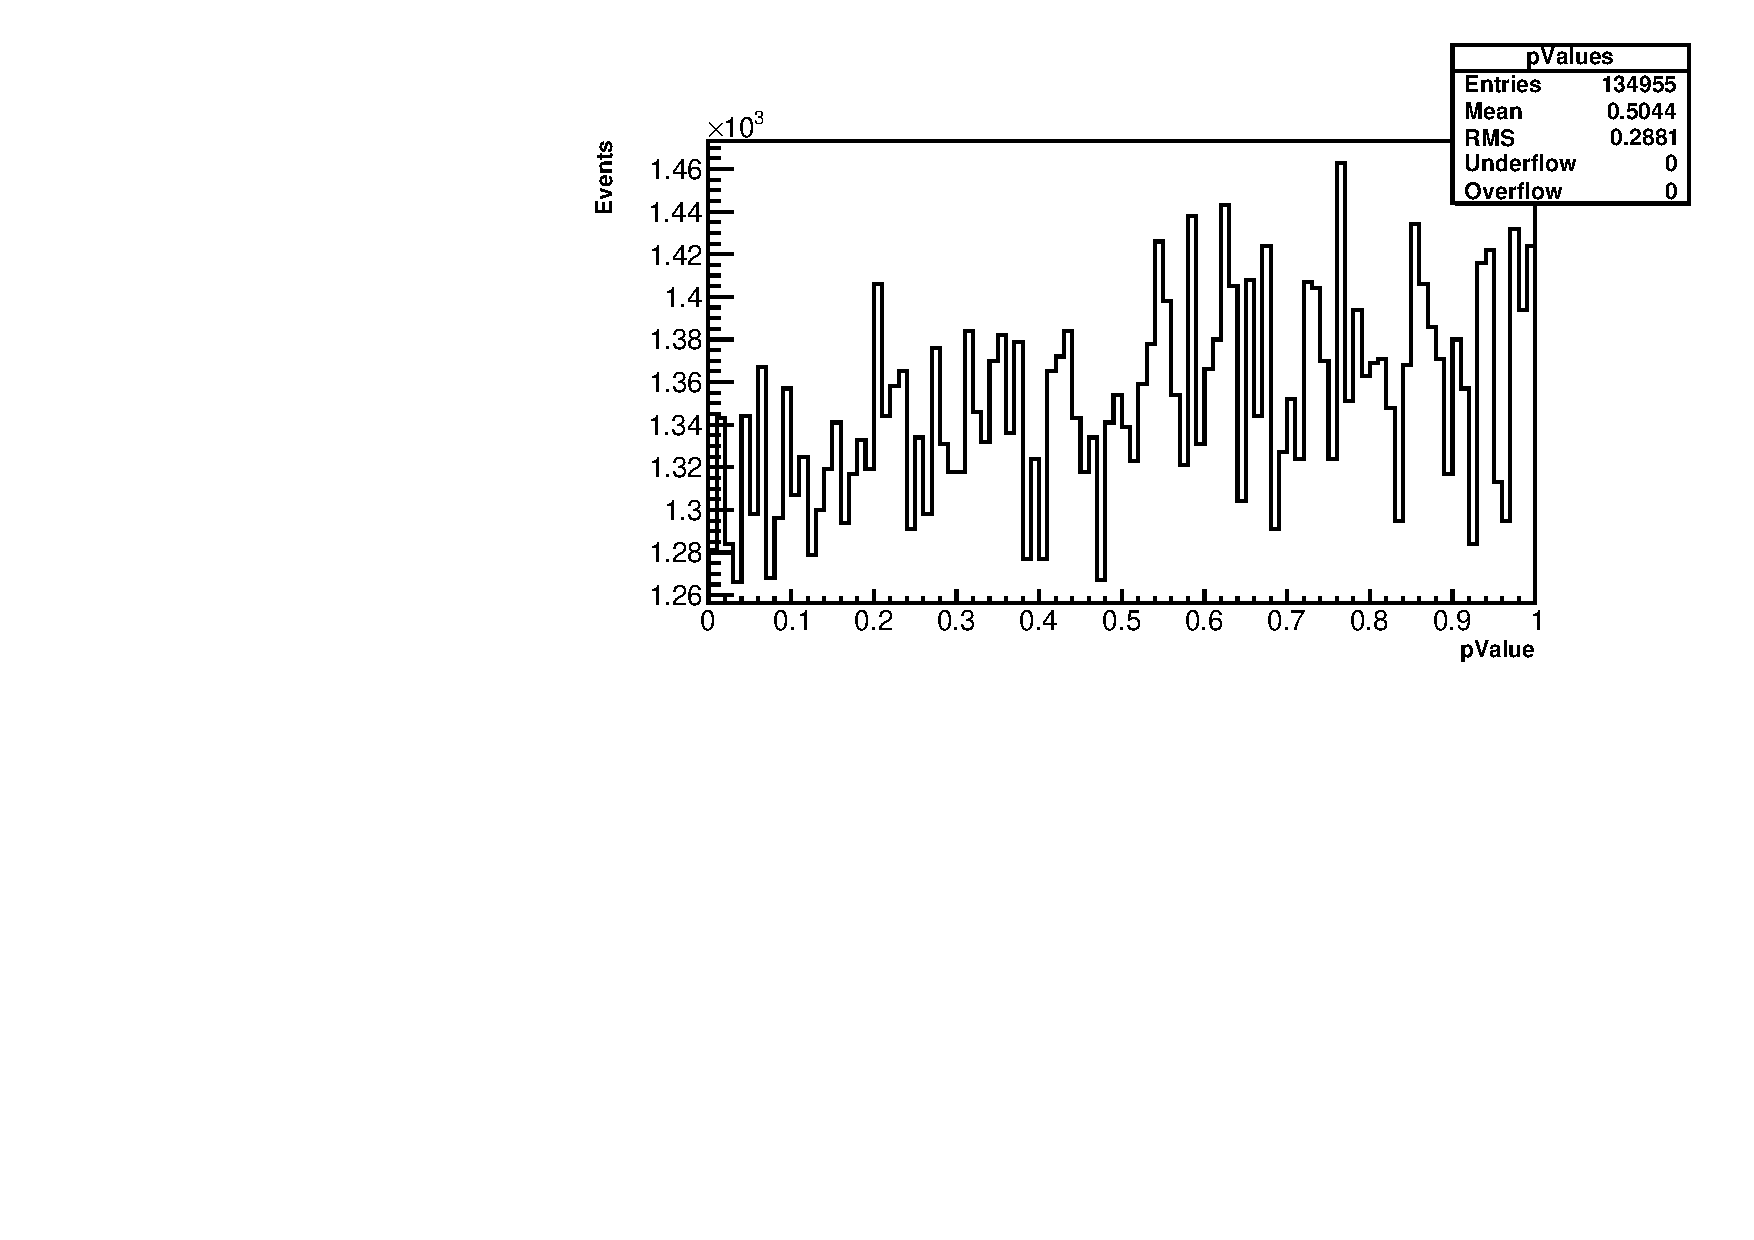
\includegraphics[width=1\textwidth]{pValueZoomed} 
        \caption{P-value distribution zoomed in. A slight rise towards 1 can be seen.}
    \end{subfigure}

    \caption{$\chi^{2}$ and p-value distributions for all tracks. There are less entries than in \ref{fig:worked} due to the energy cut of 3 MeV.}
\end{figure}



\begin{figure}
    \centering
    \begin{subfigure}[]{0.65\textwidth}
        \centering
        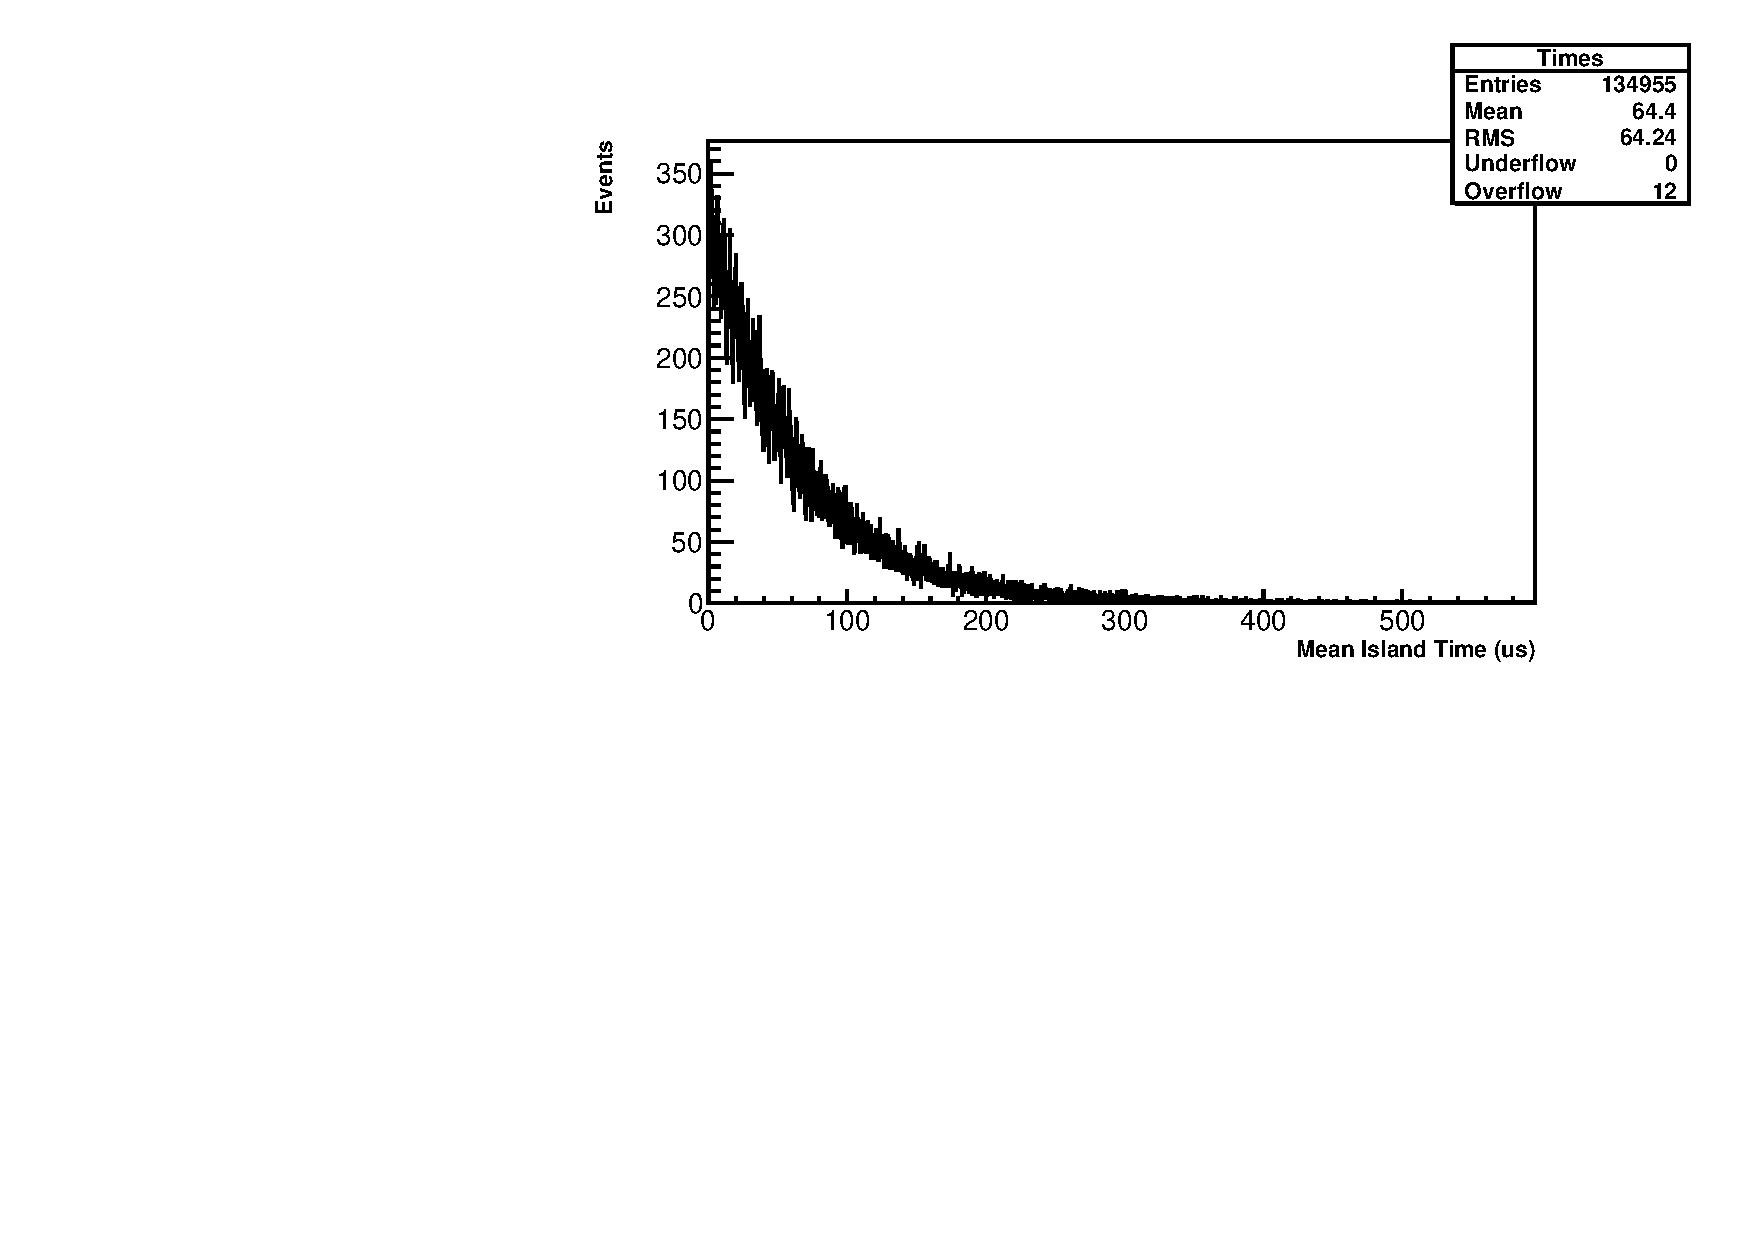
\includegraphics[width=1\textwidth]{Times} 
        \caption{Mean island times for fitted events from the mdc1 simulation. The cbo can just barely be seen.}
    \end{subfigure}
    
    \begin{subfigure}[]{0.65\textwidth}
        \centering
        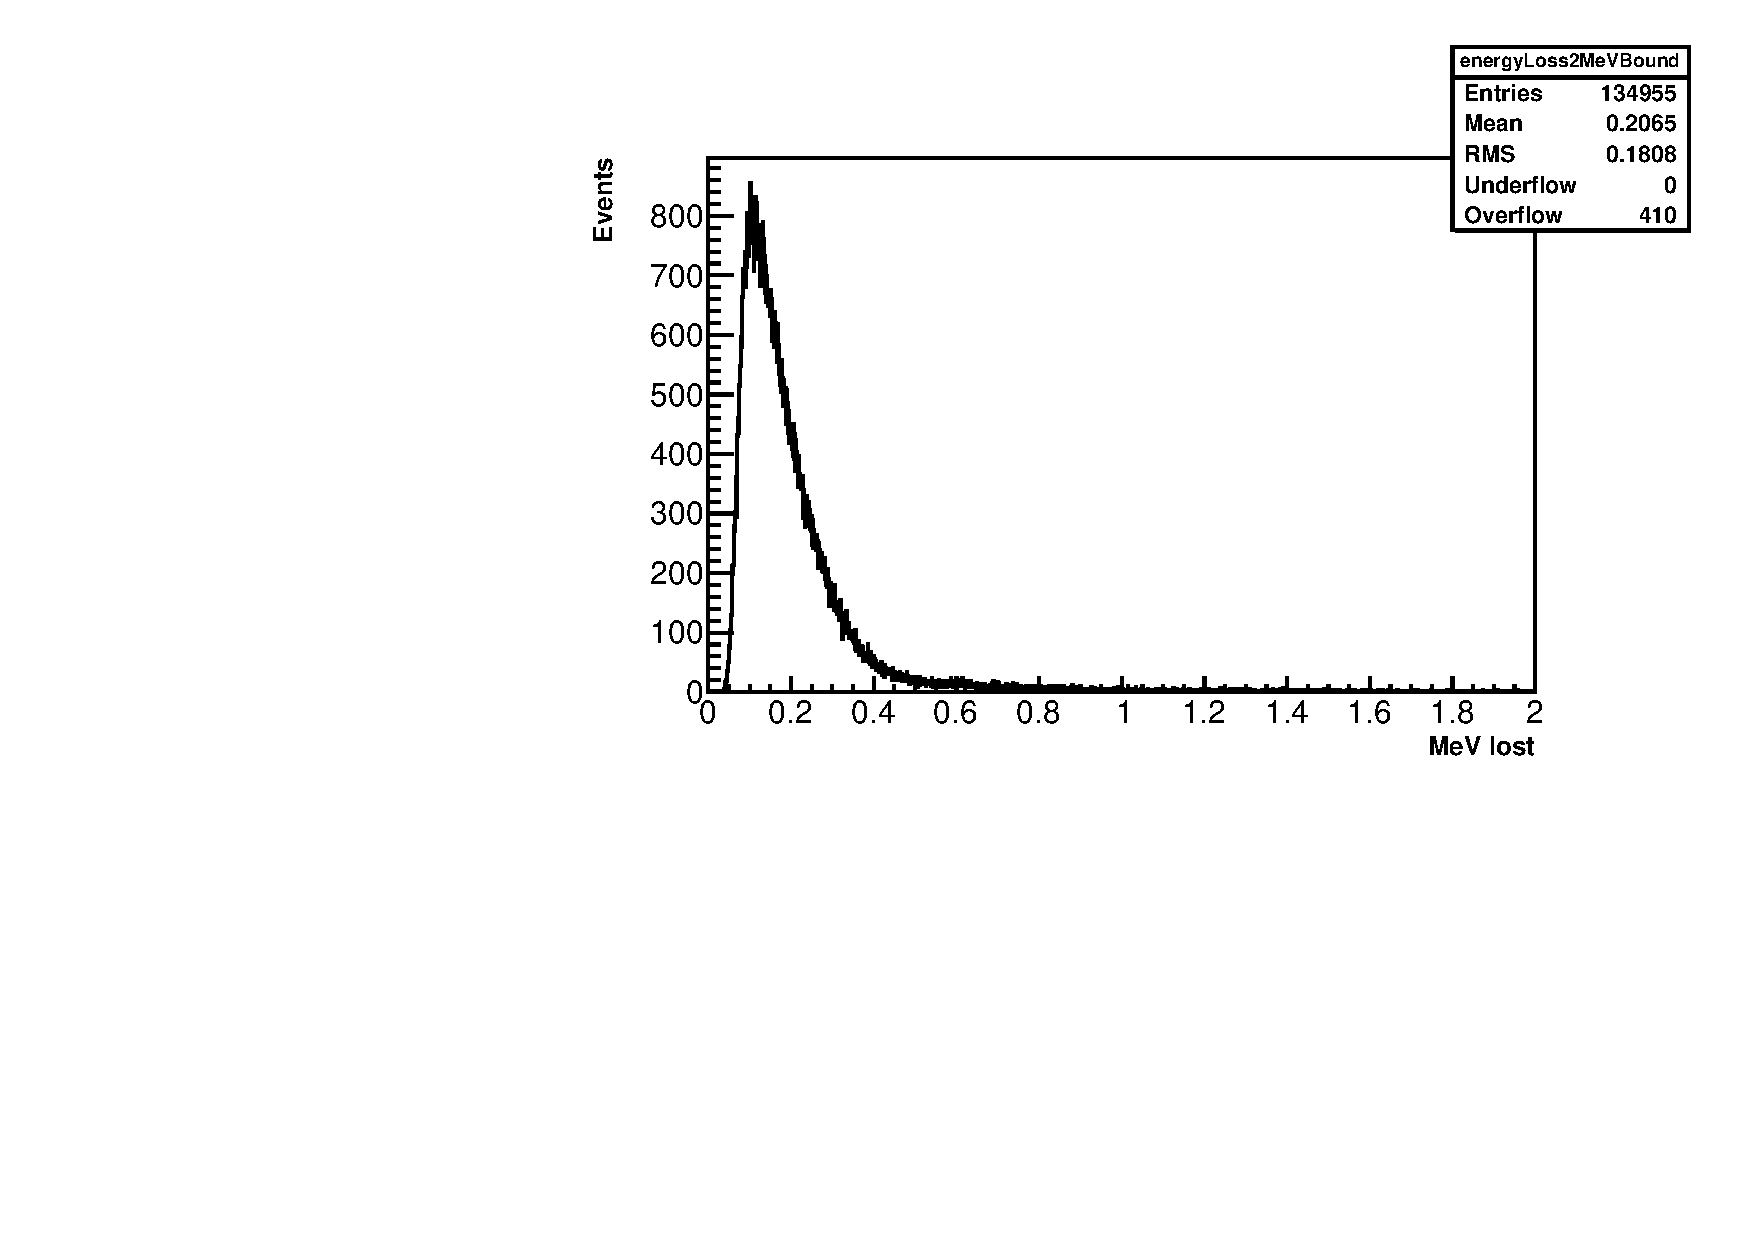
\includegraphics[width=1\textwidth]{trueEnergyLoss} 
        \caption{True energy loss between the first and last hit in the tracker. Peaks at about 120 keV with a mean of about 200 keV.}
    \end{subfigure}

    \begin{subfigure}[]{0.65\textwidth}
        \centering
        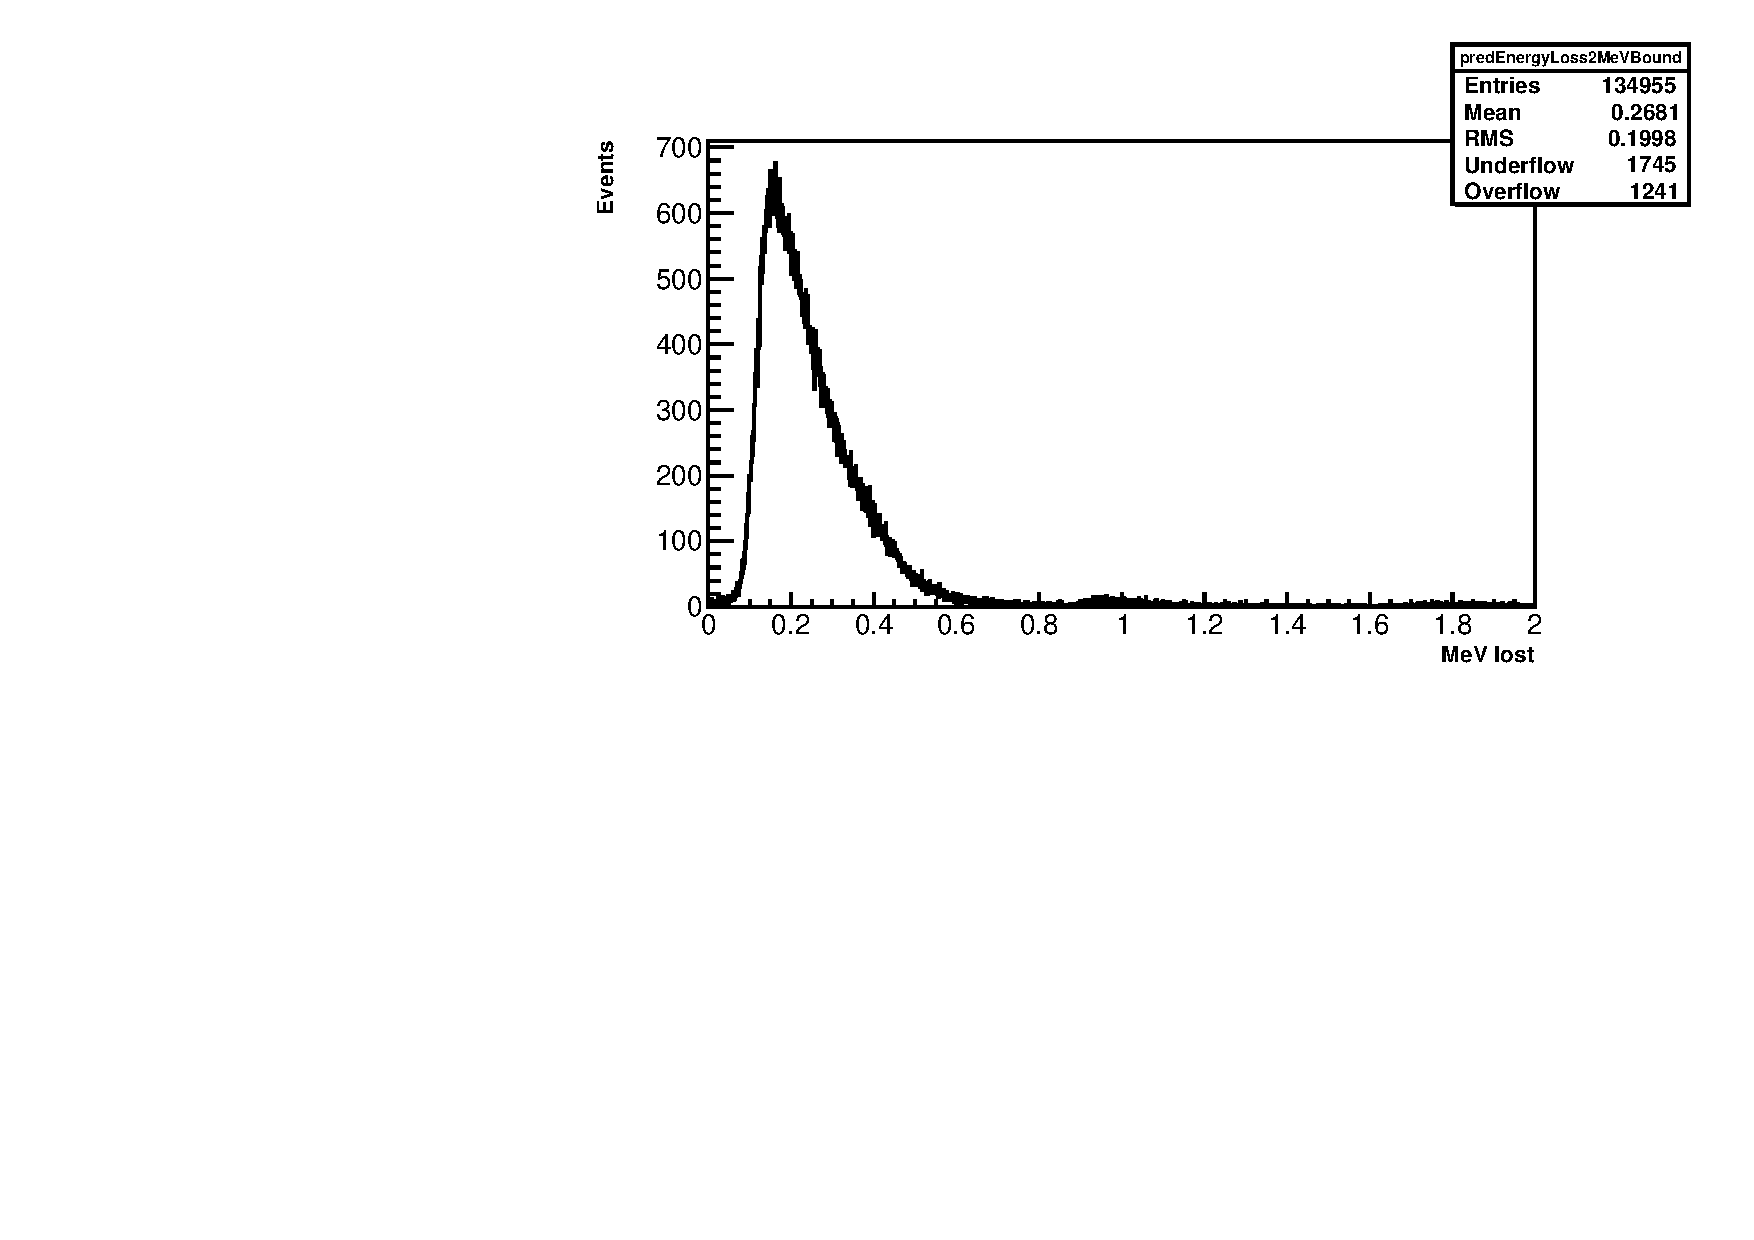
\includegraphics[width=1\textwidth]{predEnergyLoss} 
        \caption{Predicted energy loss from Geane fitting. Peaks at about 150 keV with a mean of about 270 keV. There is a slight overestimation of energy loss from truth. This is pretty negligble, but can probably be improved if necessary.}
    \end{subfigure}

    \caption{Energy and time information of the fitted tracks.}
\end{figure}



\begin{figure}
    \centering
    \begin{subfigure}[]{0.6\textwidth}
        \centering
        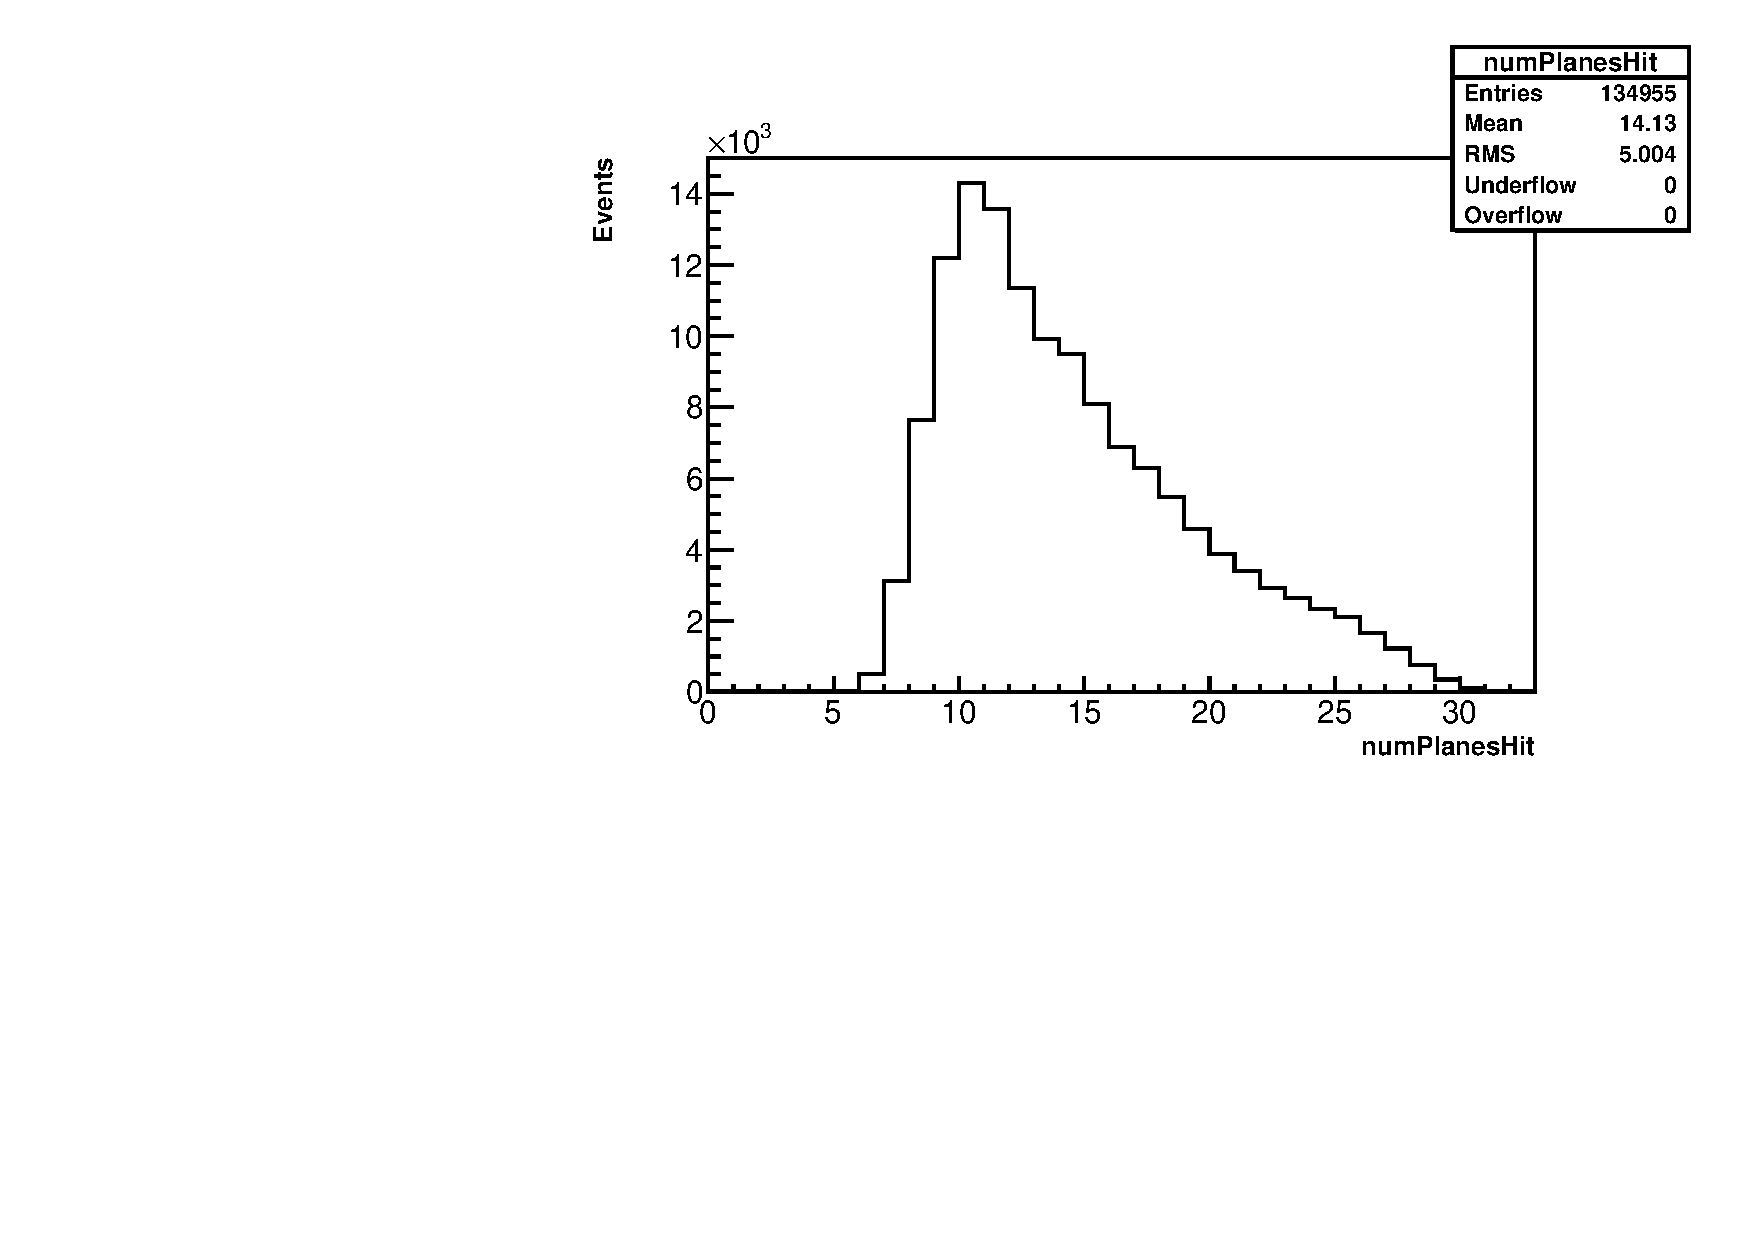
\includegraphics[width=1\textwidth]{numPlanesHit} 
        \caption{Number of planes hit per track. Peaks at 11 and falls off steadily.}
    \end{subfigure}
    
    \begin{subfigure}[]{0.6\textwidth}
        \centering
        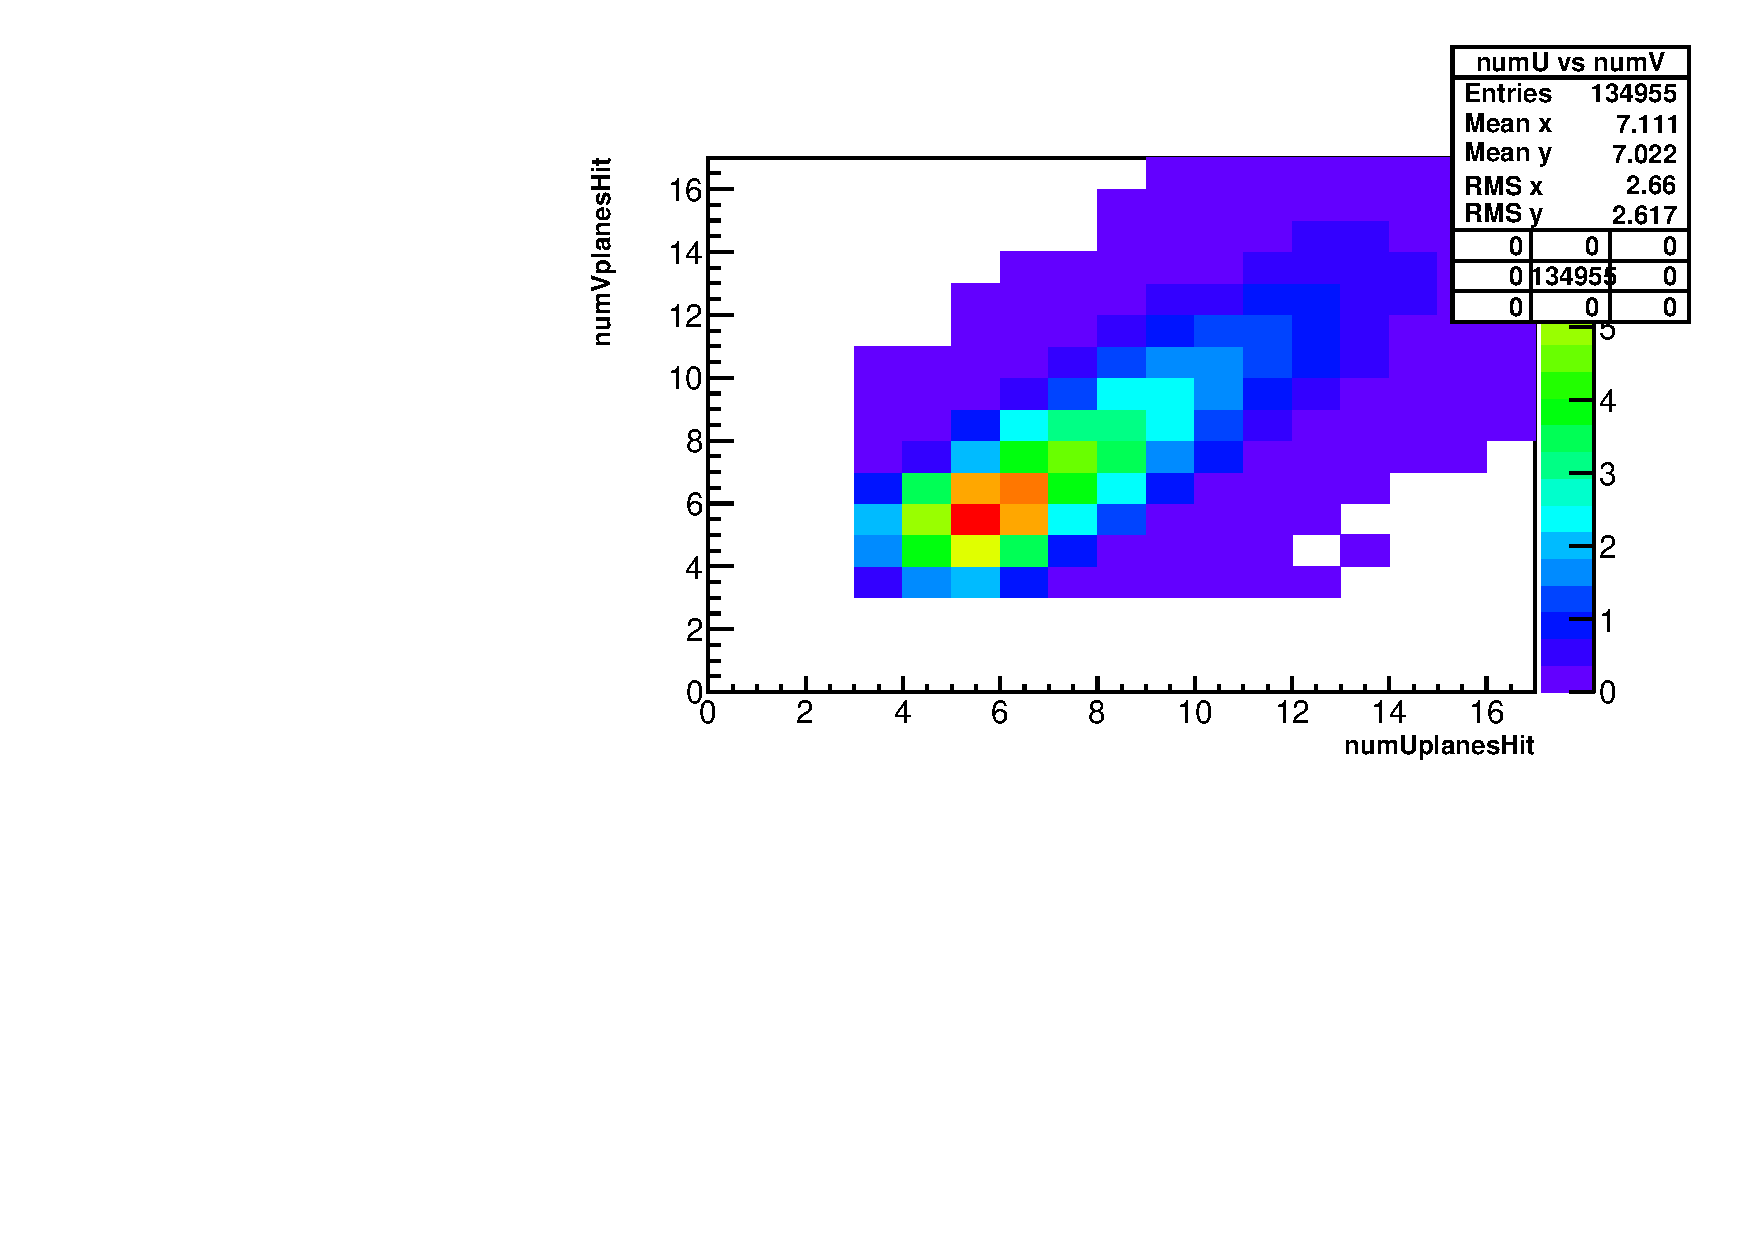
\includegraphics[width=1\textwidth]{numUnumV} 
        \caption{Number of U planes hit vs the number of V planes hit.}
    \end{subfigure}

    \begin{subfigure}[]{0.6\textwidth}
        \centering
        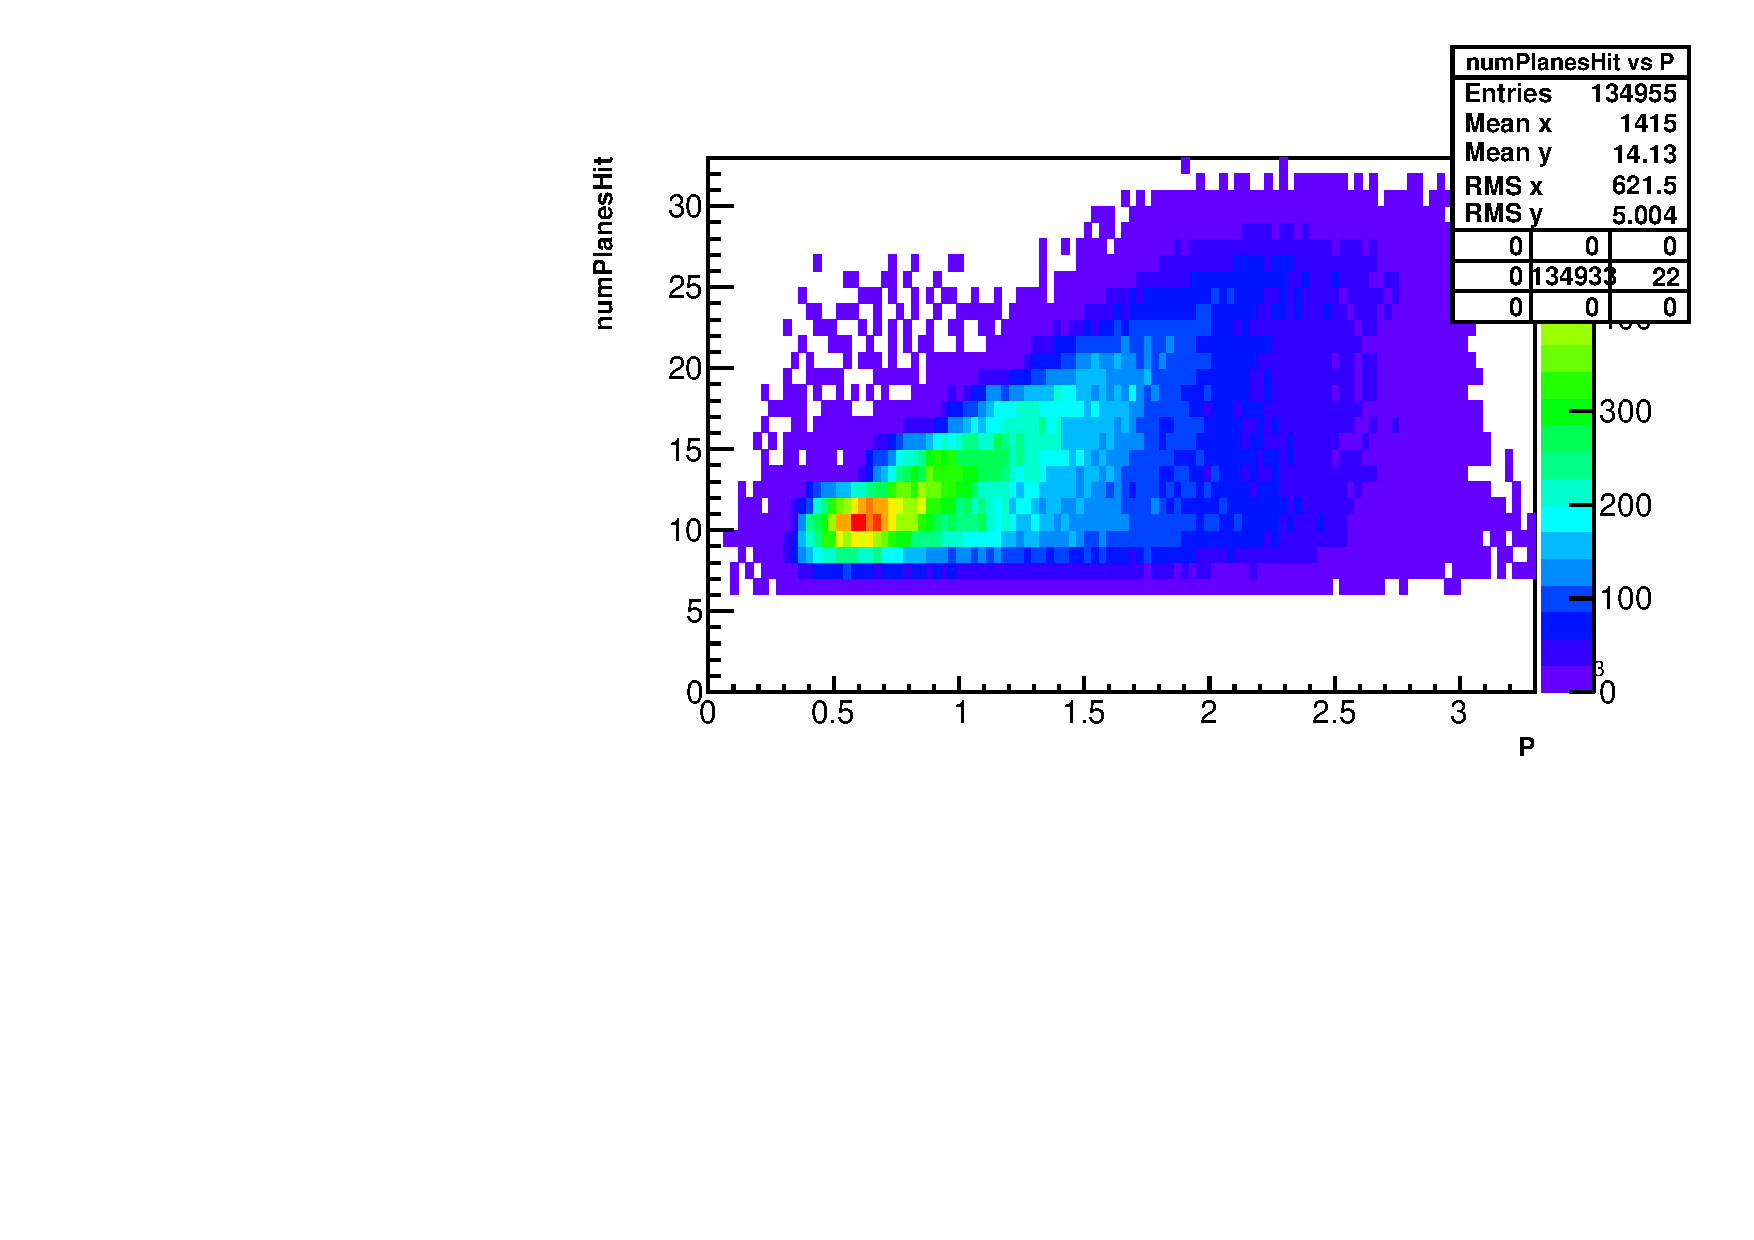
\includegraphics[width=1\textwidth]{numHitvsP} 
        \caption{Number of planes hit vs track momentum. These variables are very correlated, the higher the momentum of the track, the more likely it is to hit more planes.}
    \end{subfigure}

    \caption{Number of planes hit information.}
\end{figure}



\begin{figure}
    \centering
    \begin{subfigure}[]{0.8\textwidth}
        \centering
        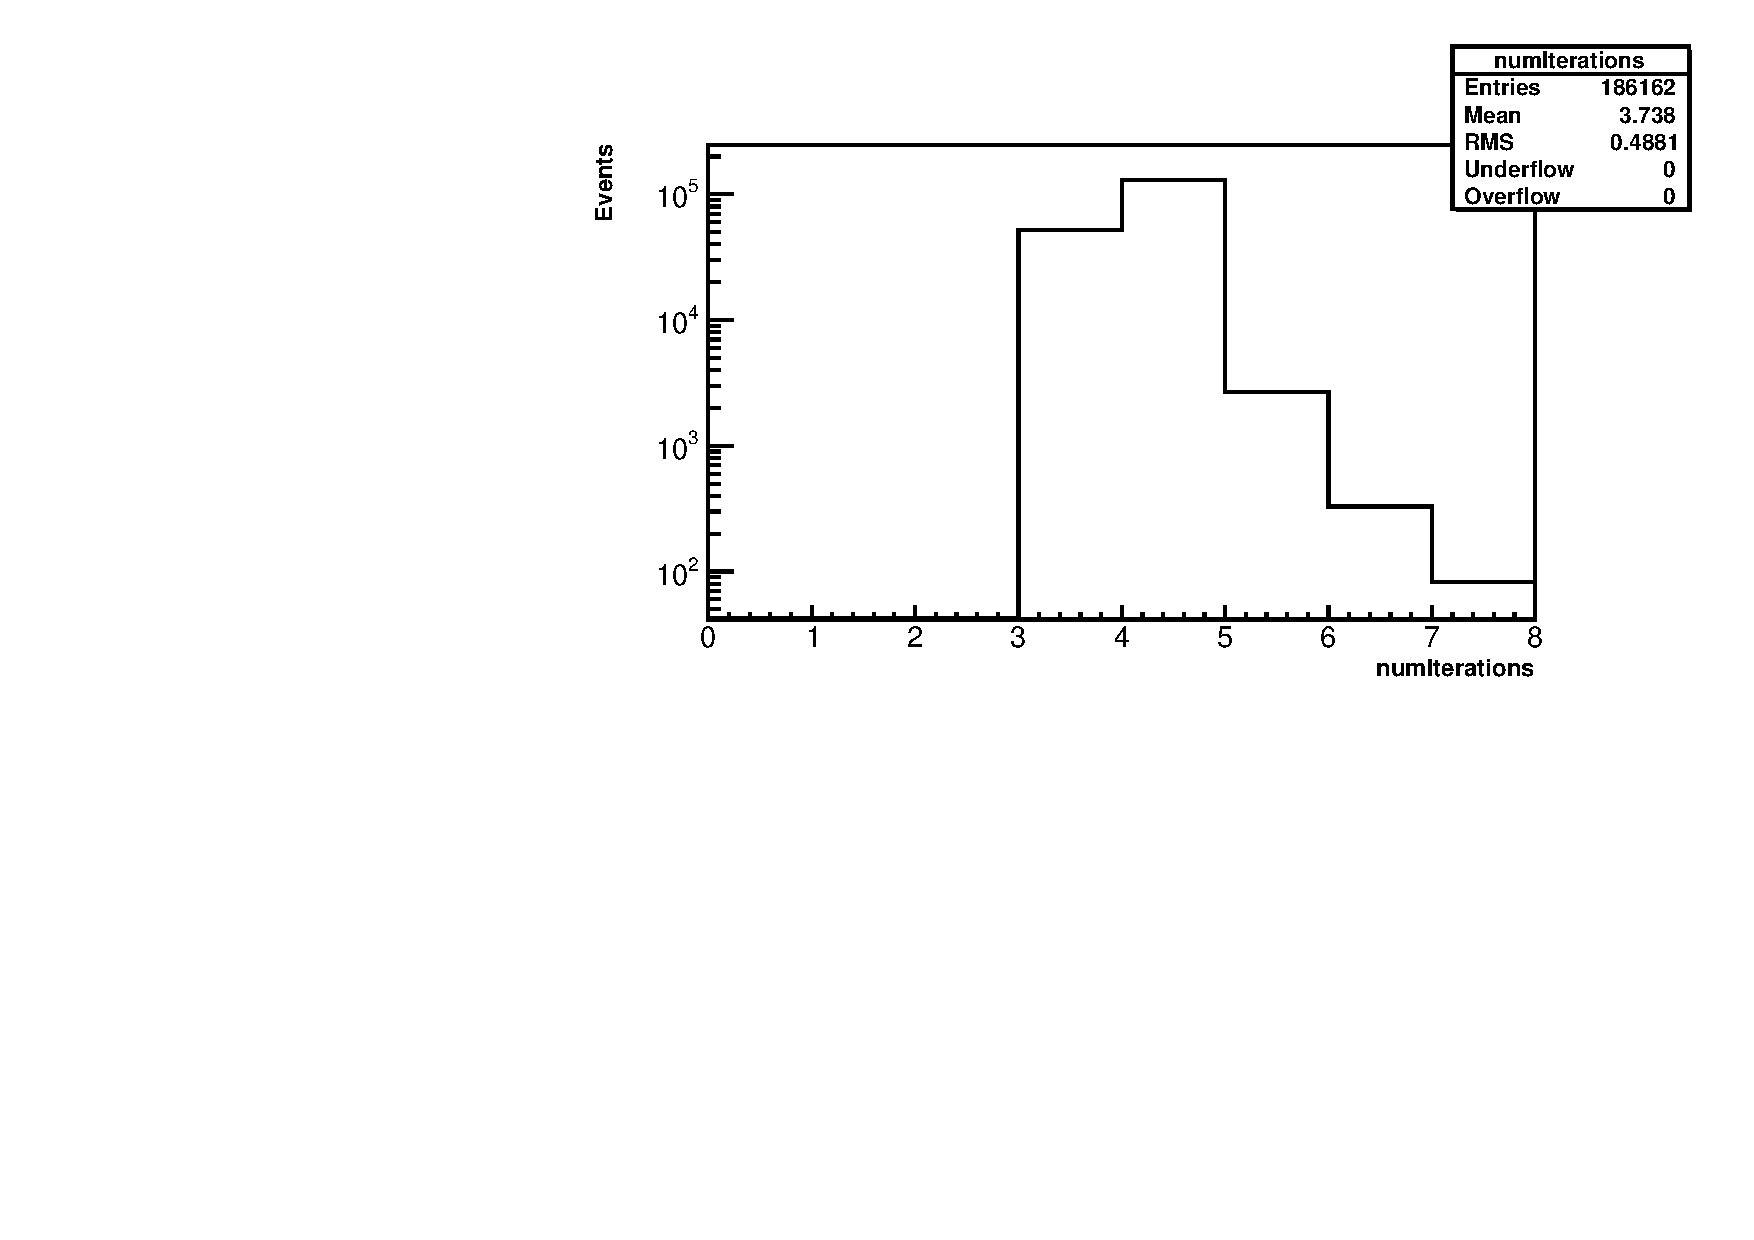
\includegraphics[width=1\textwidth]{numIterations} 
        \caption{Number of iterations to fit the track. Peaks at 4 with not less than 3 iterations.}
    \end{subfigure}
    
    \begin{subfigure}[]{0.8\textwidth}
        \centering
        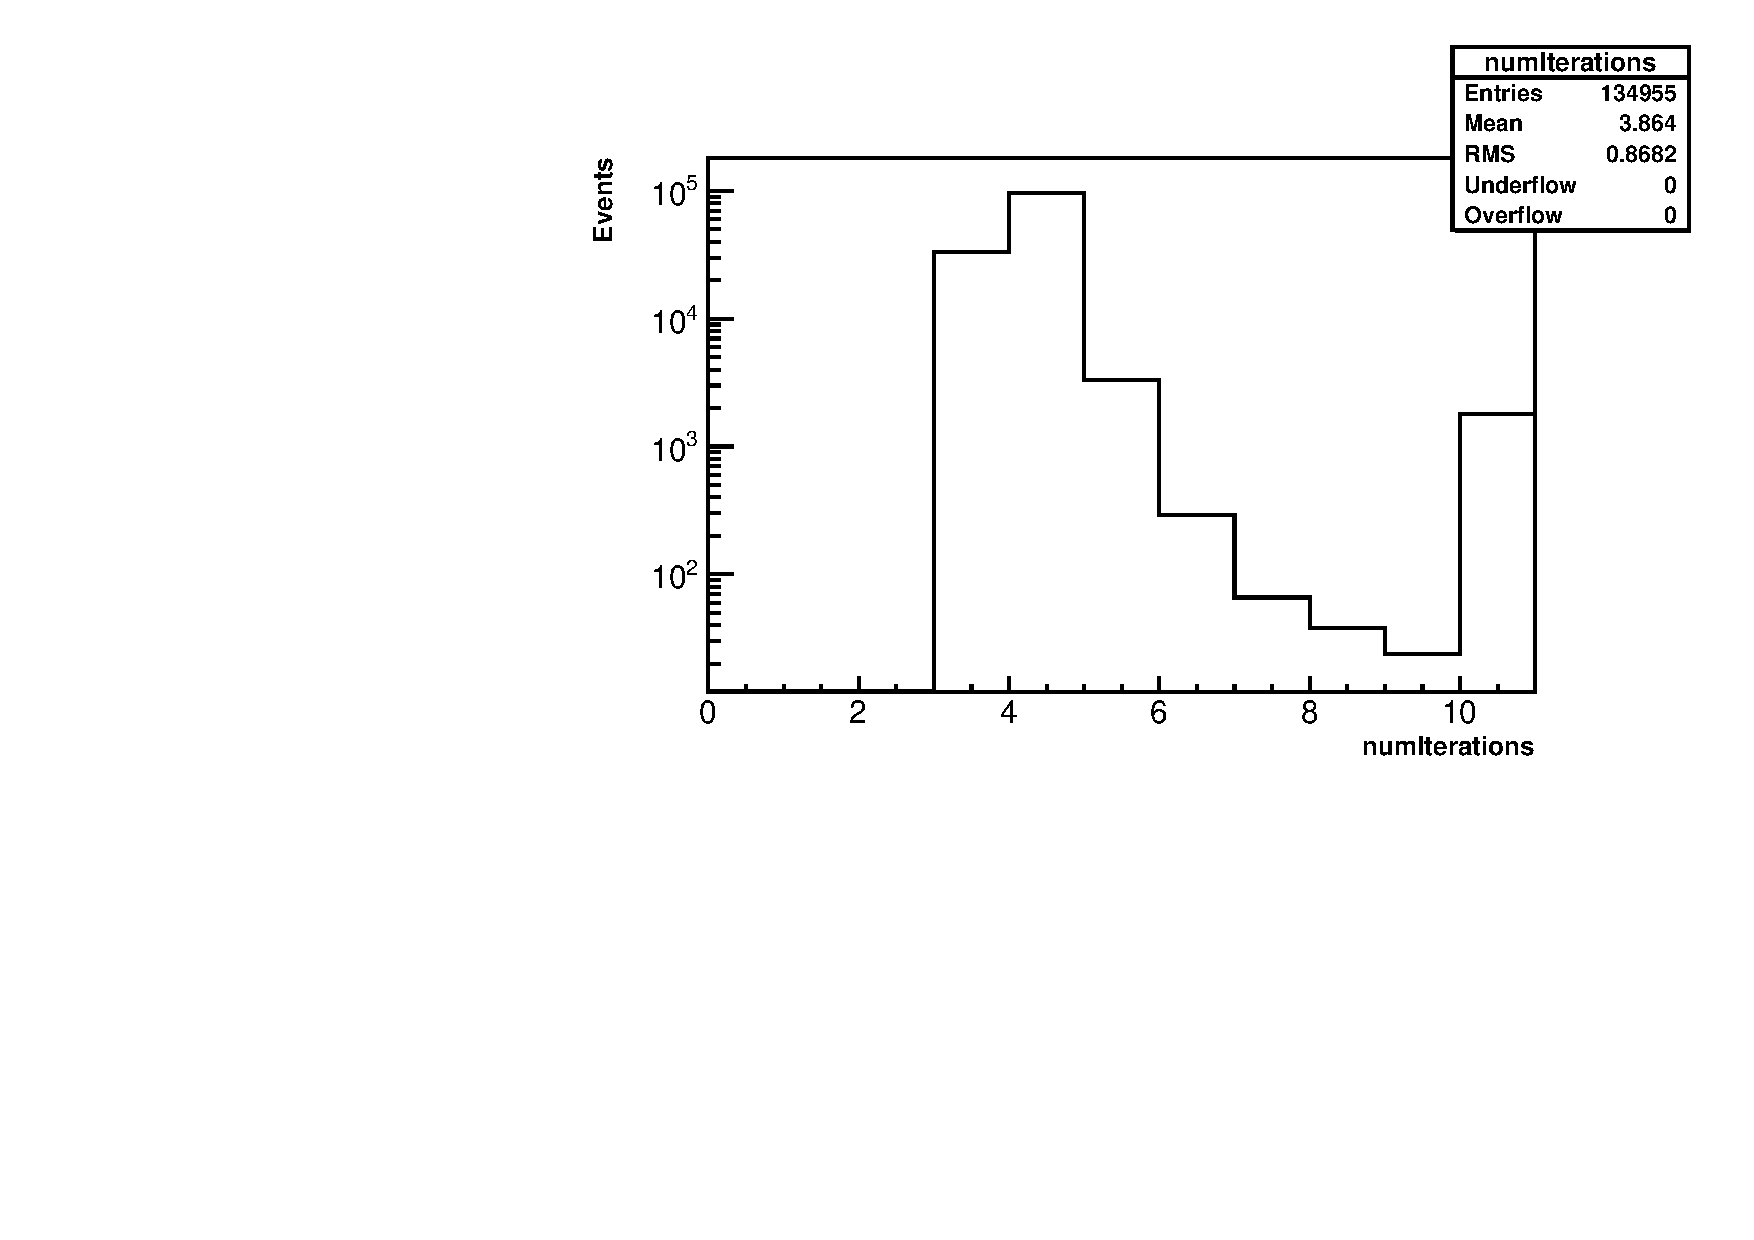
\includegraphics[width=1\textwidth]{numIterationsLog} 
        \caption{Number of iterations log plot. The number of iterations is manually cut off at 10, which is why there is an increase in the last bin and no overflows.}
    \end{subfigure}

    \caption{Number of iterations information.}
\end{figure}



\begin{figure}
    \centering
    \begin{subfigure}[]{0.65\textwidth}
        \centering
        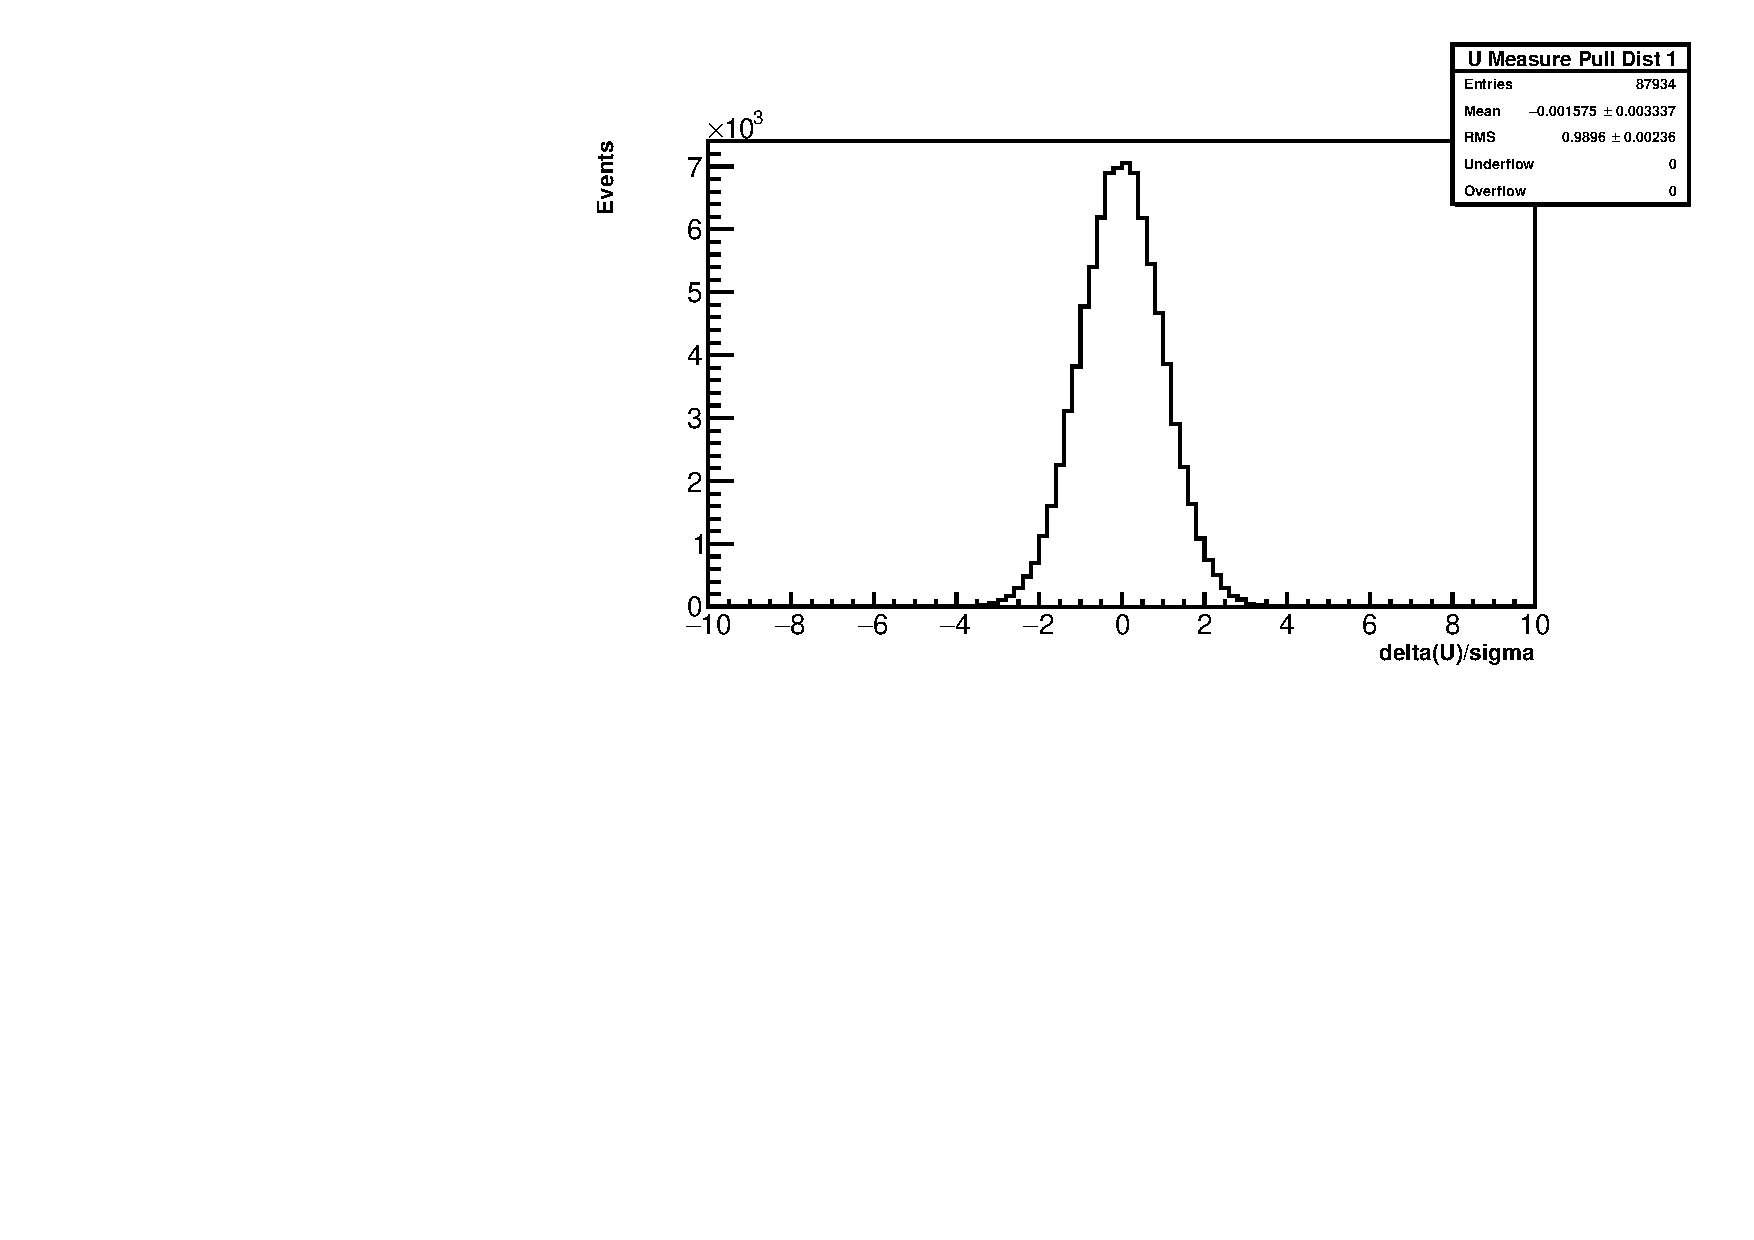
\includegraphics[width=1\textwidth]{UmeasPull} 
        \caption{U measurement pull on plane 1 as given by Equation \ref{eq:measpullmaterial}. It is a unit Gaussian within errors.}
    \end{subfigure}
    
    \begin{subfigure}[]{0.65\textwidth}
        \centering
        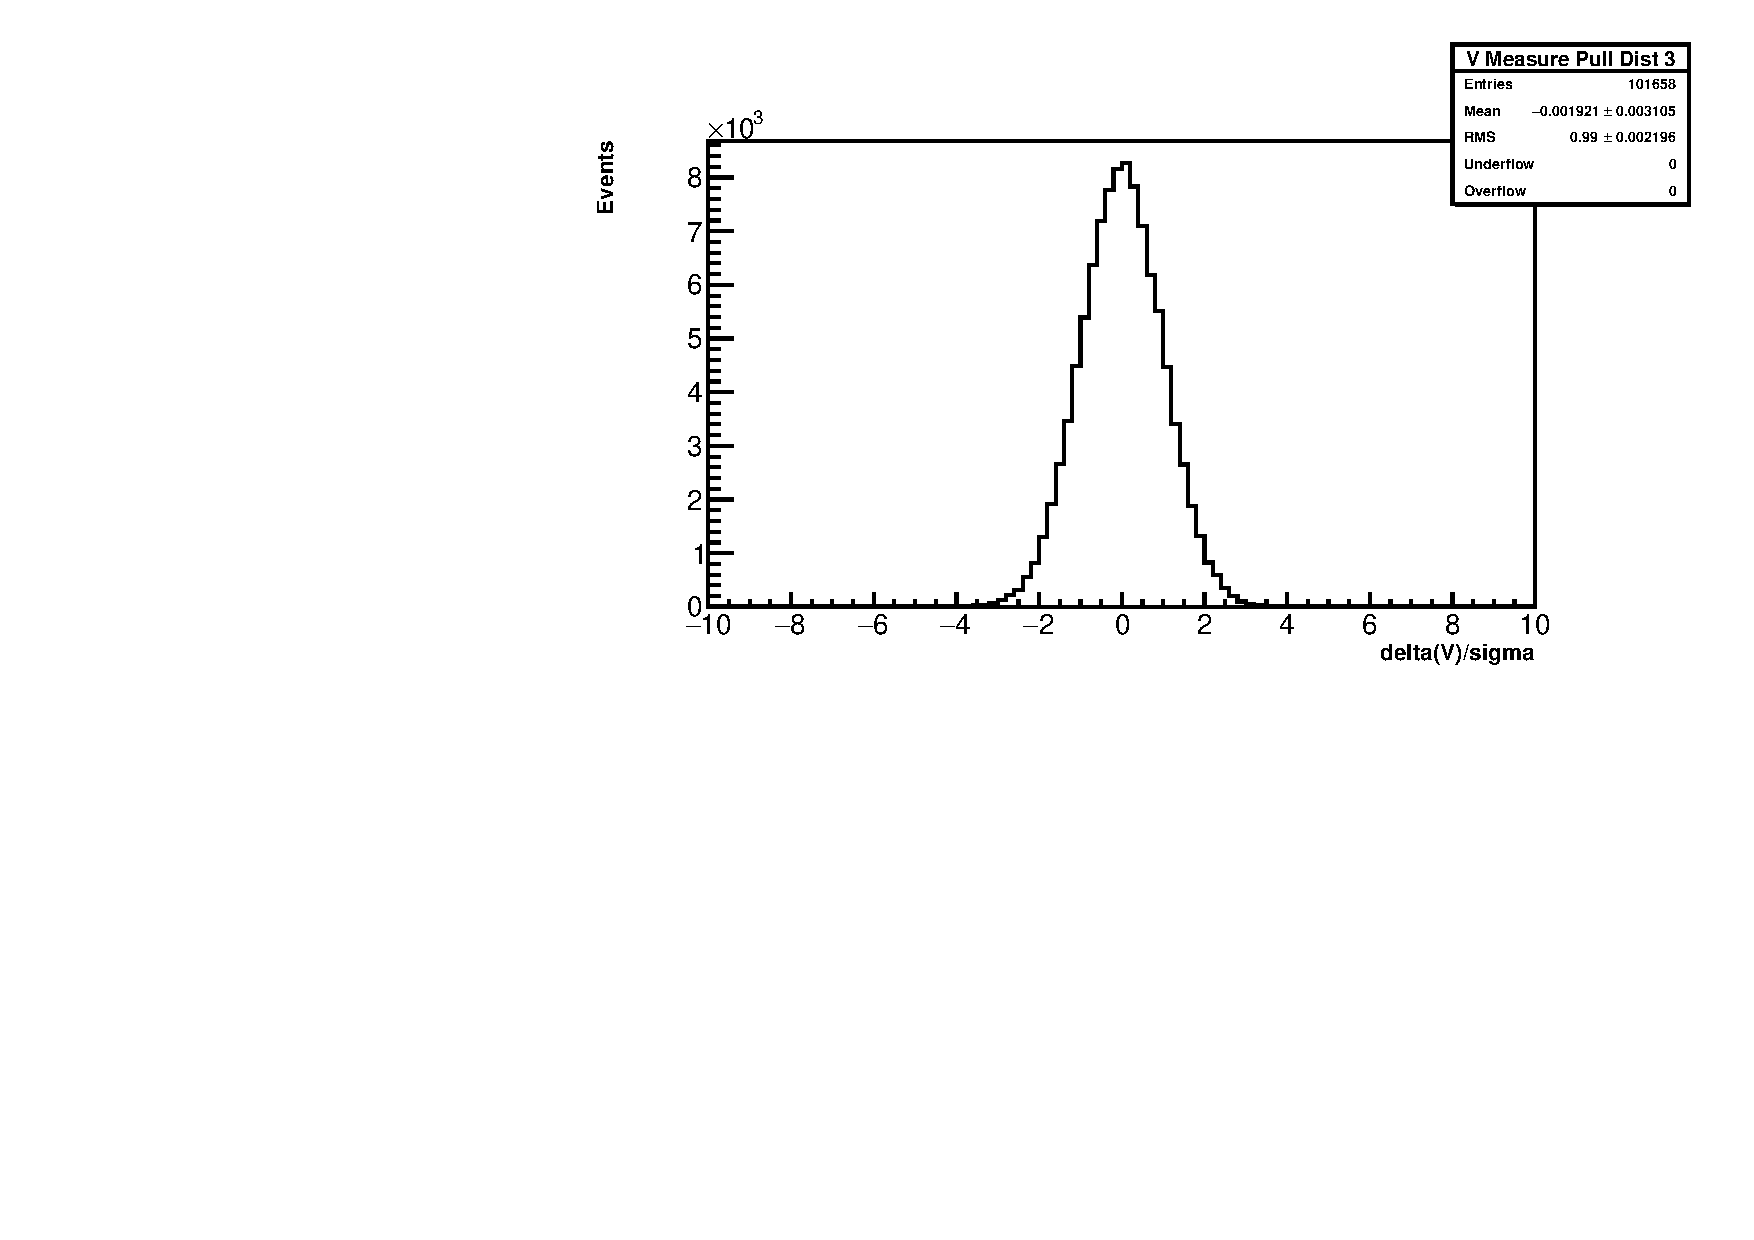
\includegraphics[width=1\textwidth]{VmeasPull} 
        \caption{V measurement pull on plane 3 as given by Equation \ref{eq:measpullmaterial}. It is a unit Gaussian within errors.}
    \end{subfigure}

    \begin{subfigure}[]{0.65\textwidth}
        \centering
        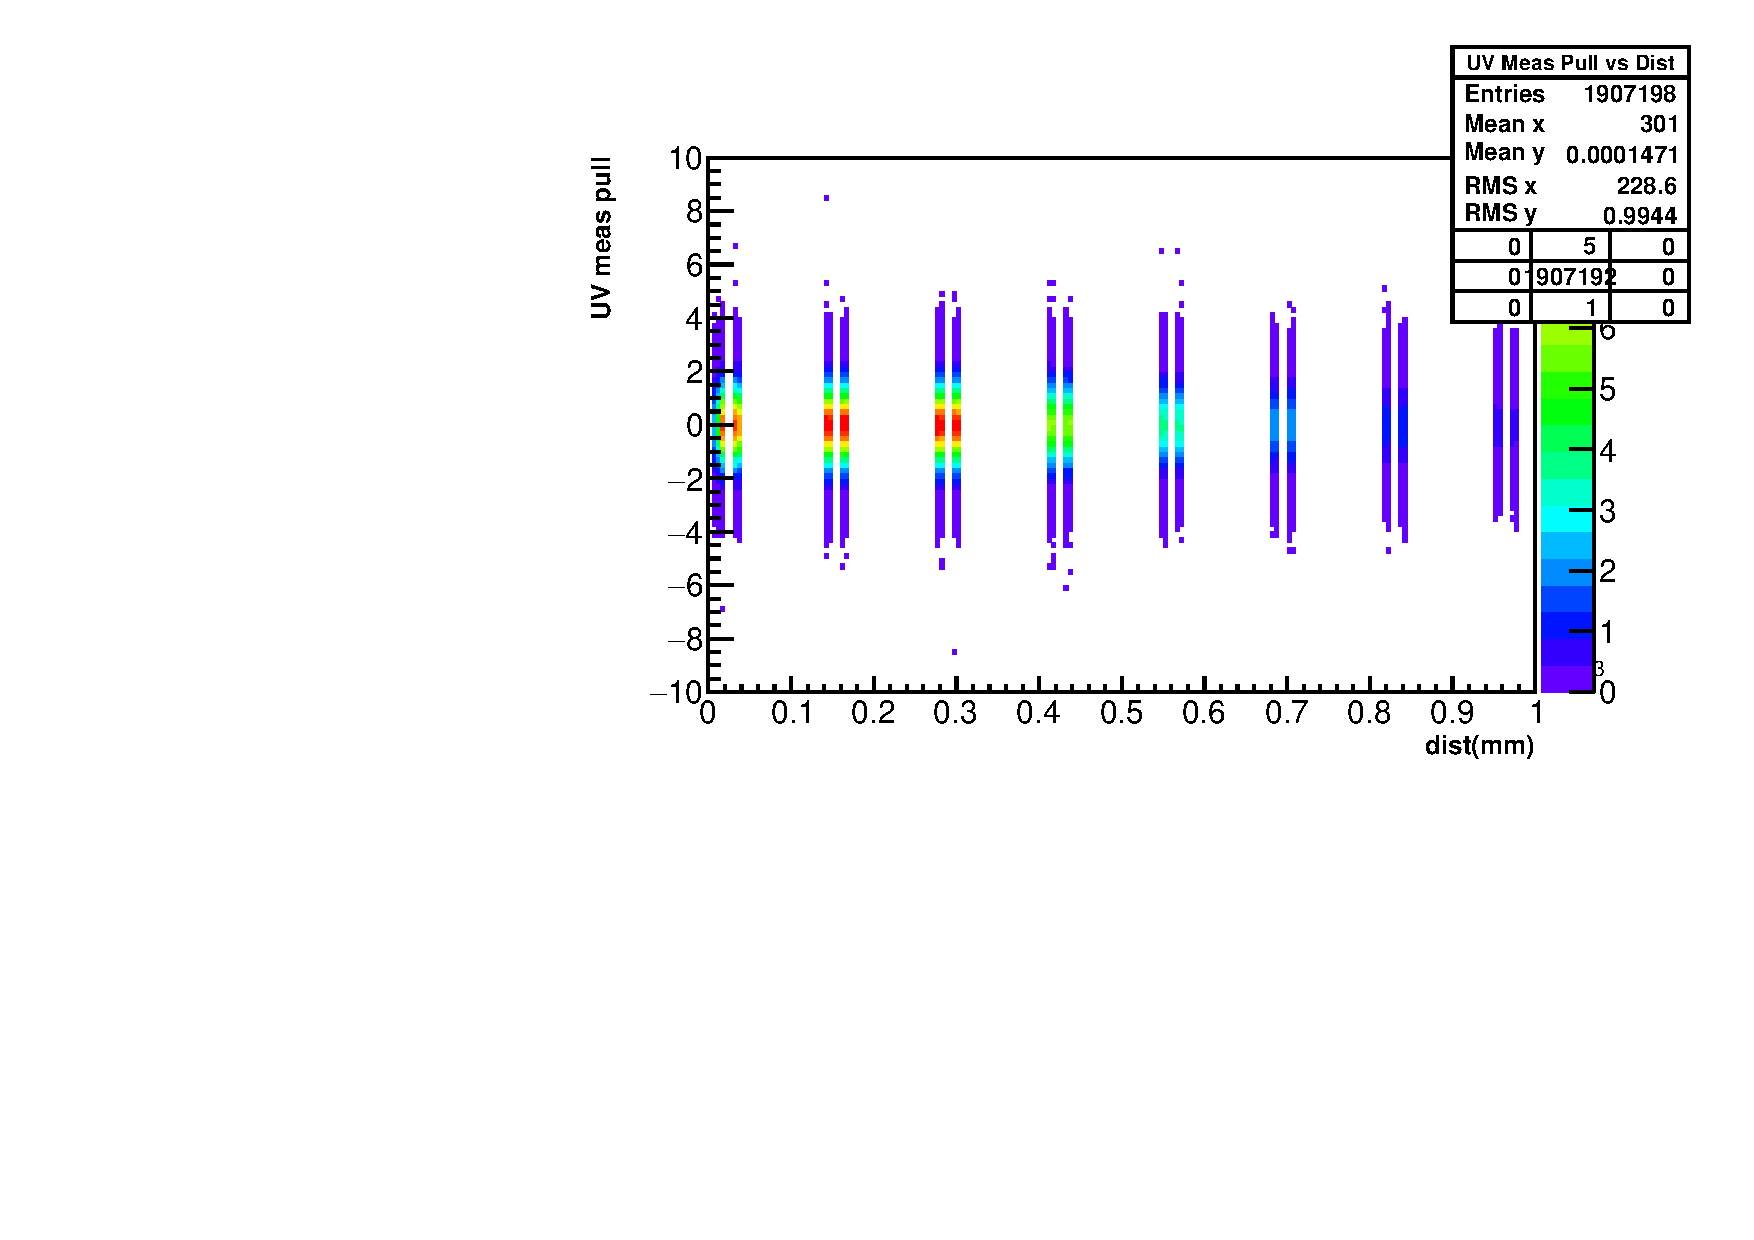
\includegraphics[width=1\textwidth]{UVMeasPullVsDist} 
        \caption{U and V measurement pulls as a function of track distance from fitting start point, or ``0'' plane. The RMS drops slightly as a function of distance, indicated imperfectly attuned errors.}
    \end{subfigure}

    \caption{Measurement pull plots, useful for track fitting on data validation.}
\end{figure}



\begin{figure}
    \centering
    \begin{subfigure}[]{0.65\textwidth}
        \centering
        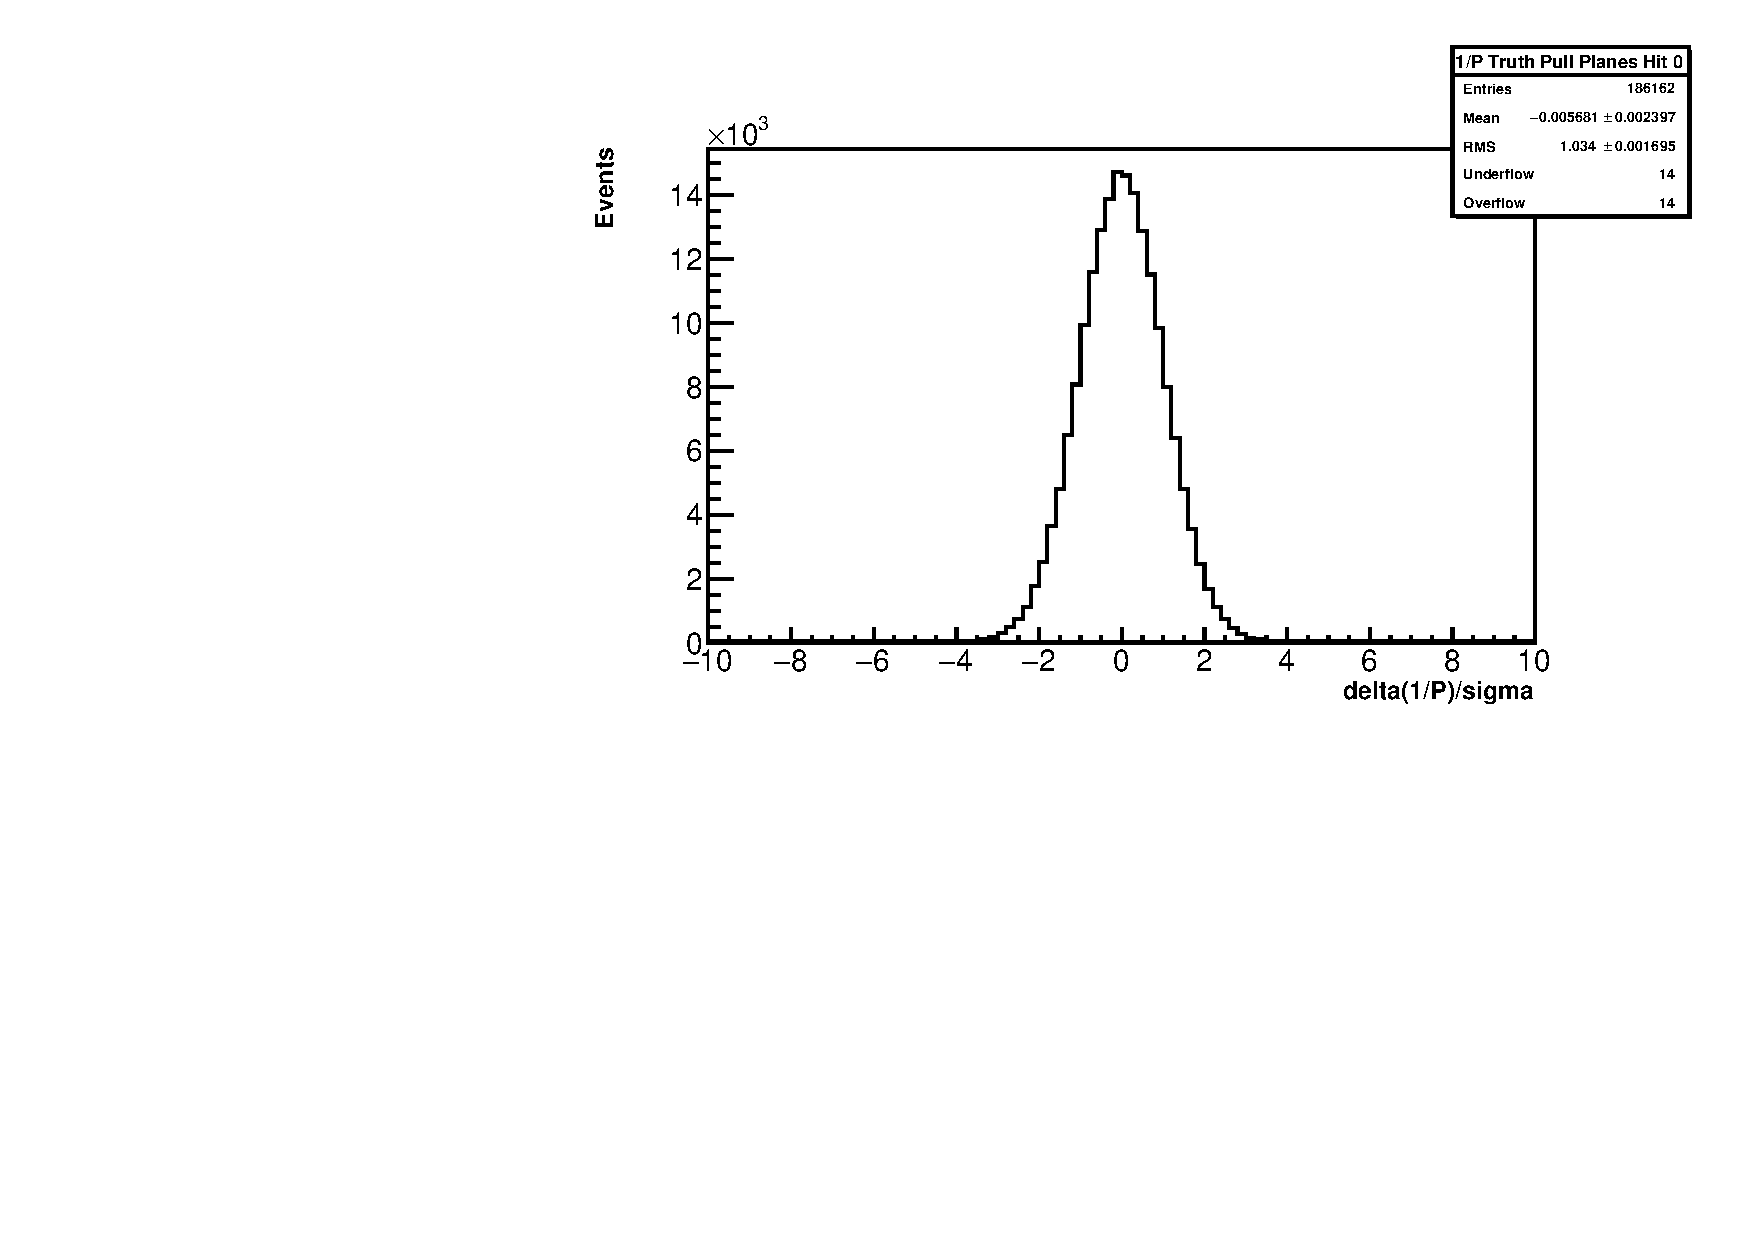
\includegraphics[width=1\textwidth]{1Ppull} 
        \caption{1/P truth pull on plane 0 for all tracks. Very close to a unit Gaussian showing the tracking is working correctly.}
    \end{subfigure}
    
    \begin{subfigure}[]{0.65\textwidth}
        \centering
        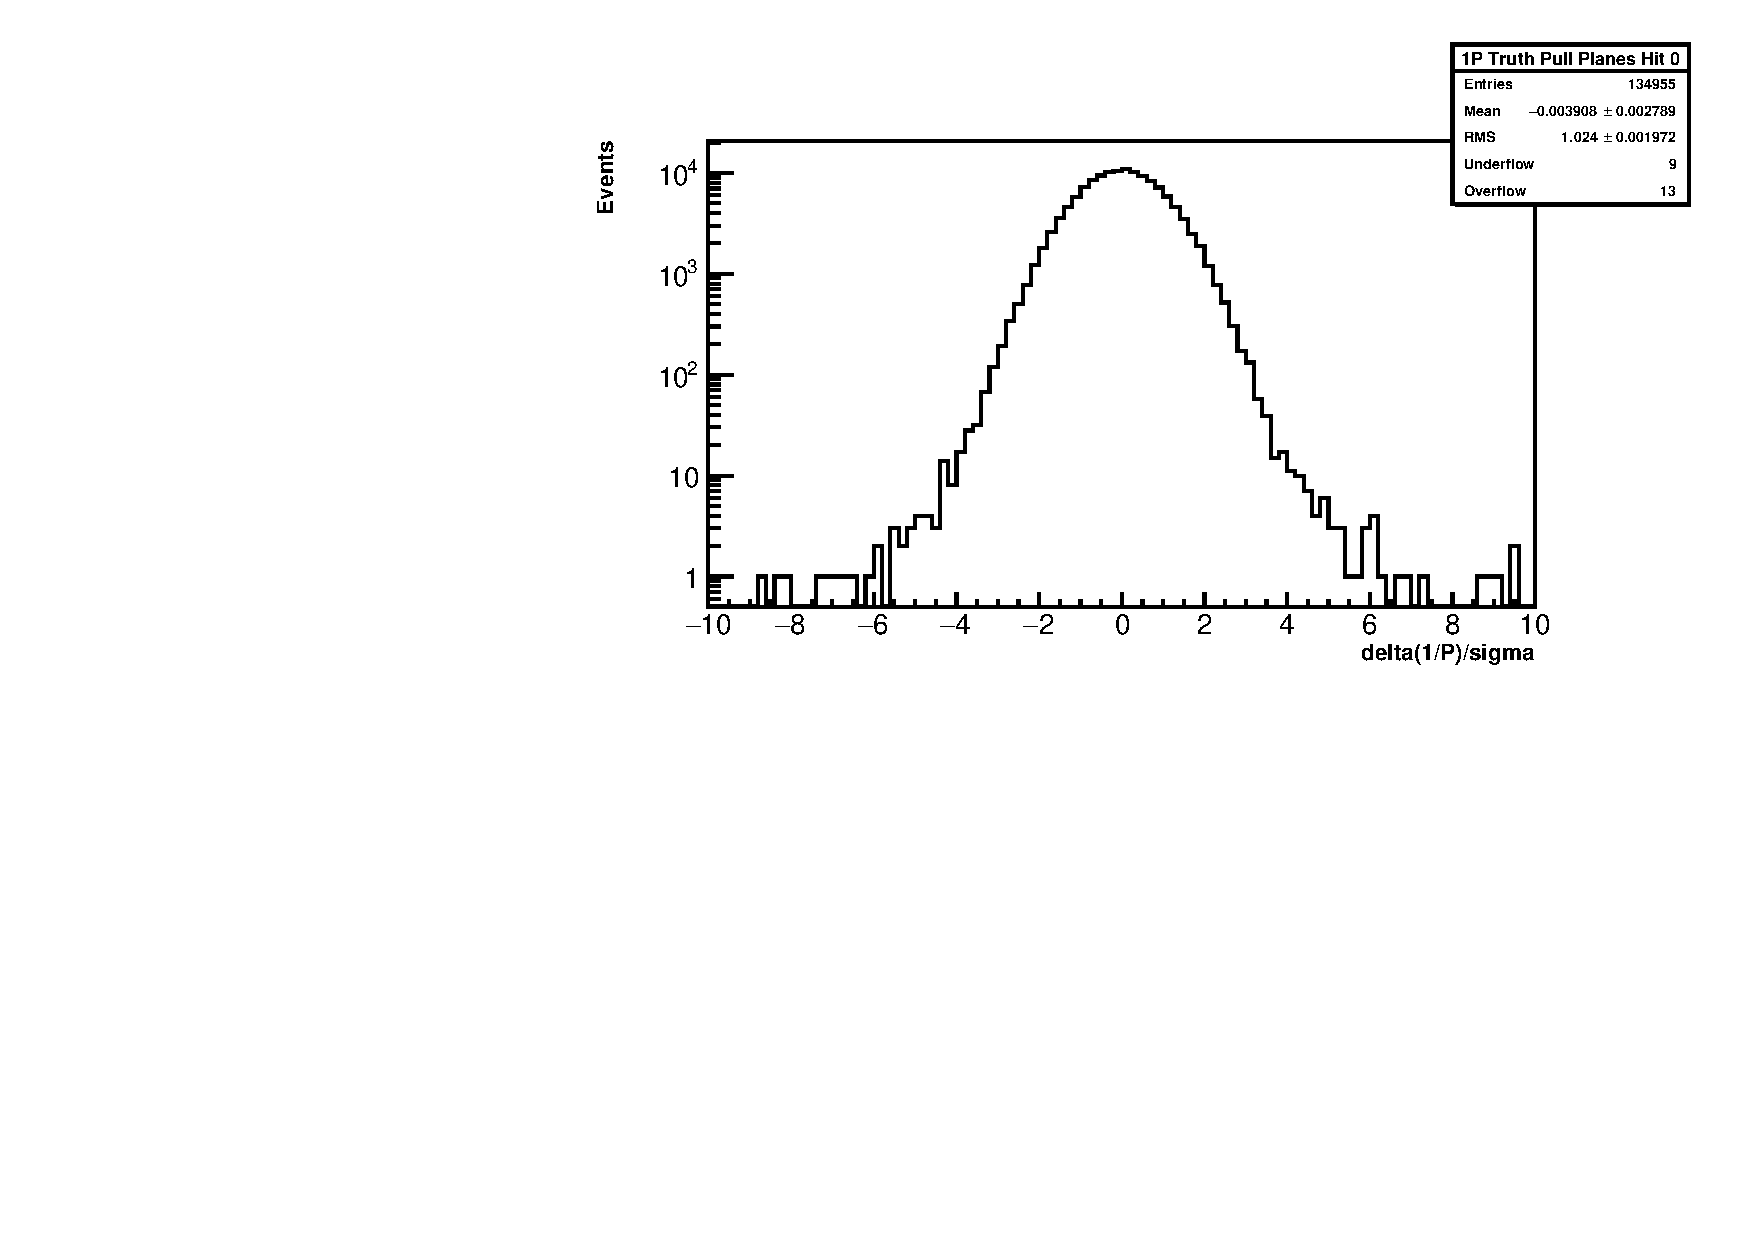
\includegraphics[width=1\textwidth]{1PpullLog} 
        \caption{1/P truth pull on plane 0 for all tracks, log plot. Poor events can be seen as the distribution spreads out more towards the edges, with some under and overflows.}
    \end{subfigure}

    \begin{subfigure}[]{0.65\textwidth}
        \centering
        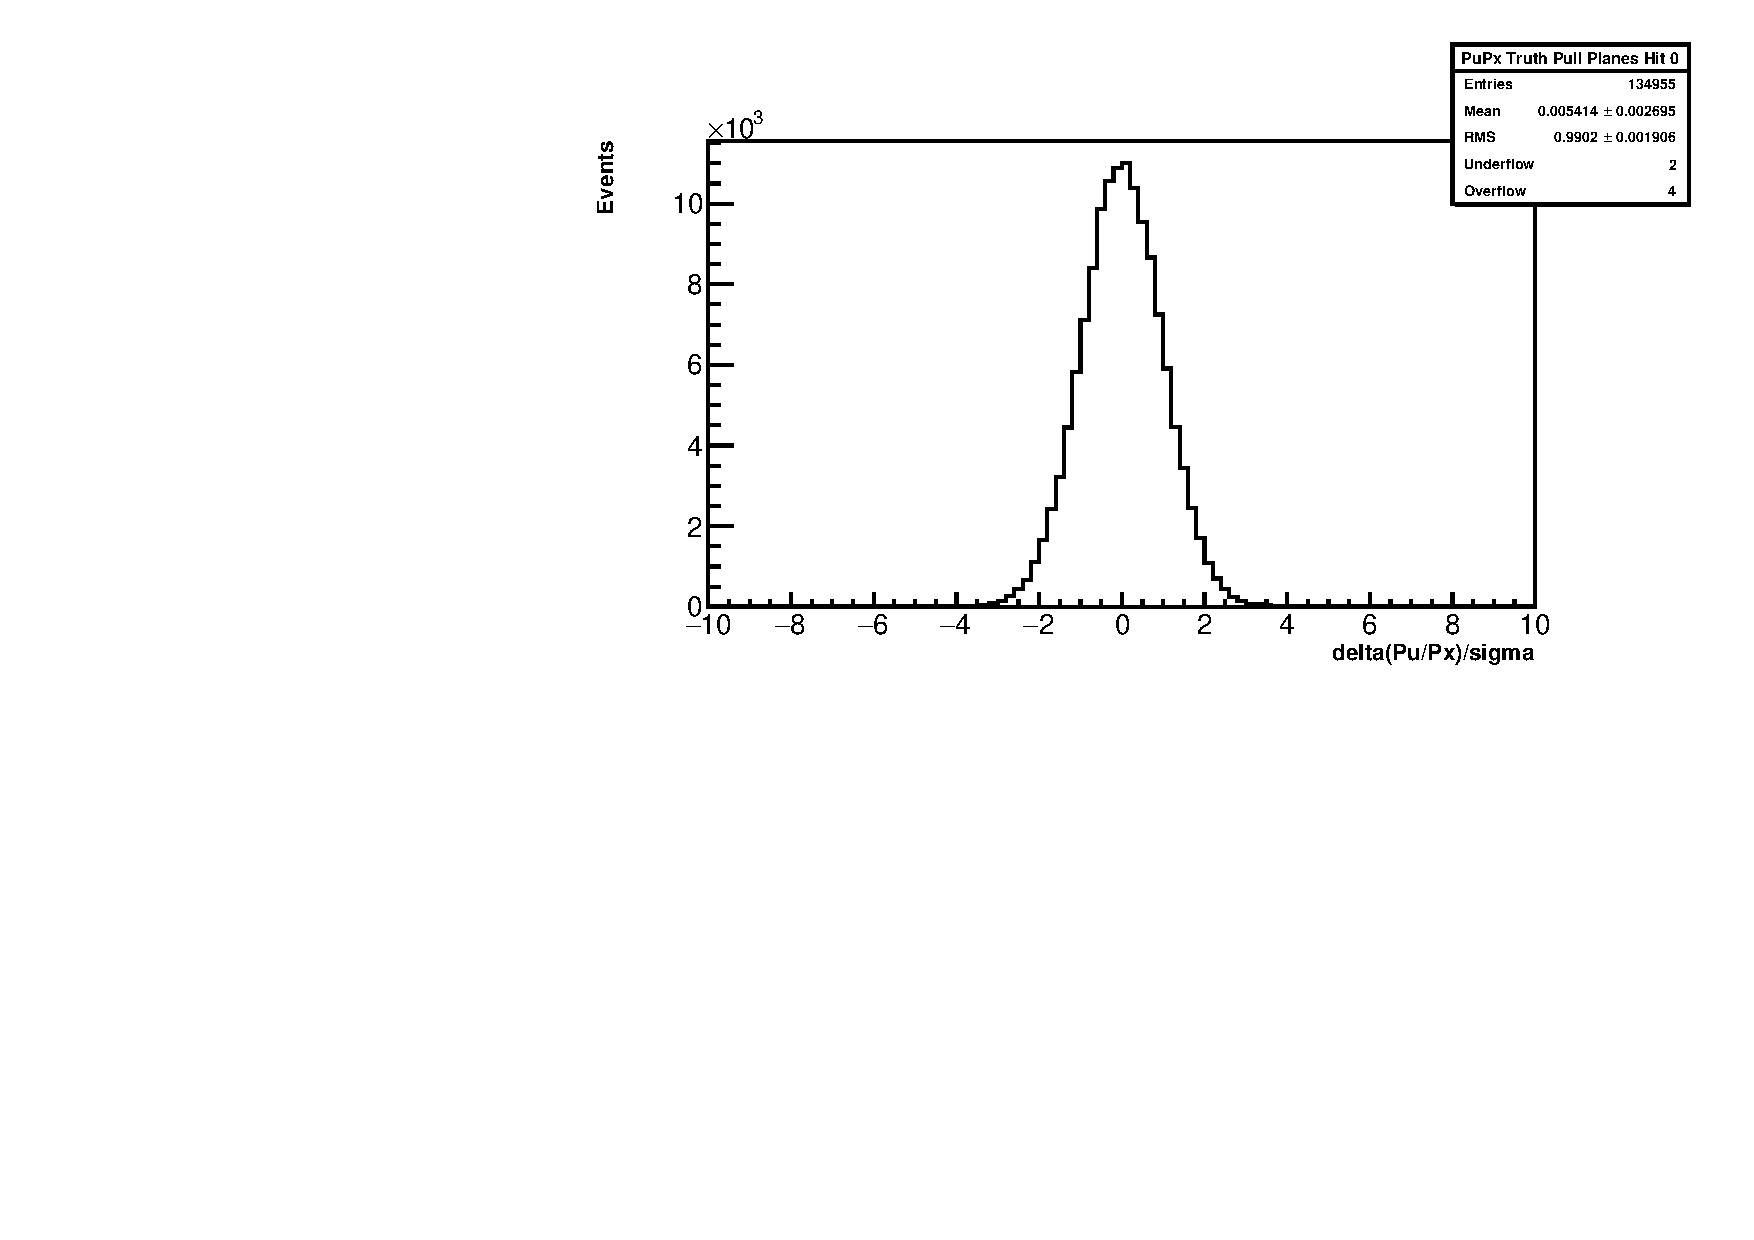
\includegraphics[width=1\textwidth]{PuPxpull} 
        \caption{Pu/Px truth pull on plane 0 for all tracks. Very close to a unit Gaussian showing the tracking is working correctly.}
    \end{subfigure}

    \caption{Truth pulls on plane 0 for all tracks.}
\end{figure}



\begin{figure}
    \centering
    \begin{subfigure}[]{0.65\textwidth}
        \centering
        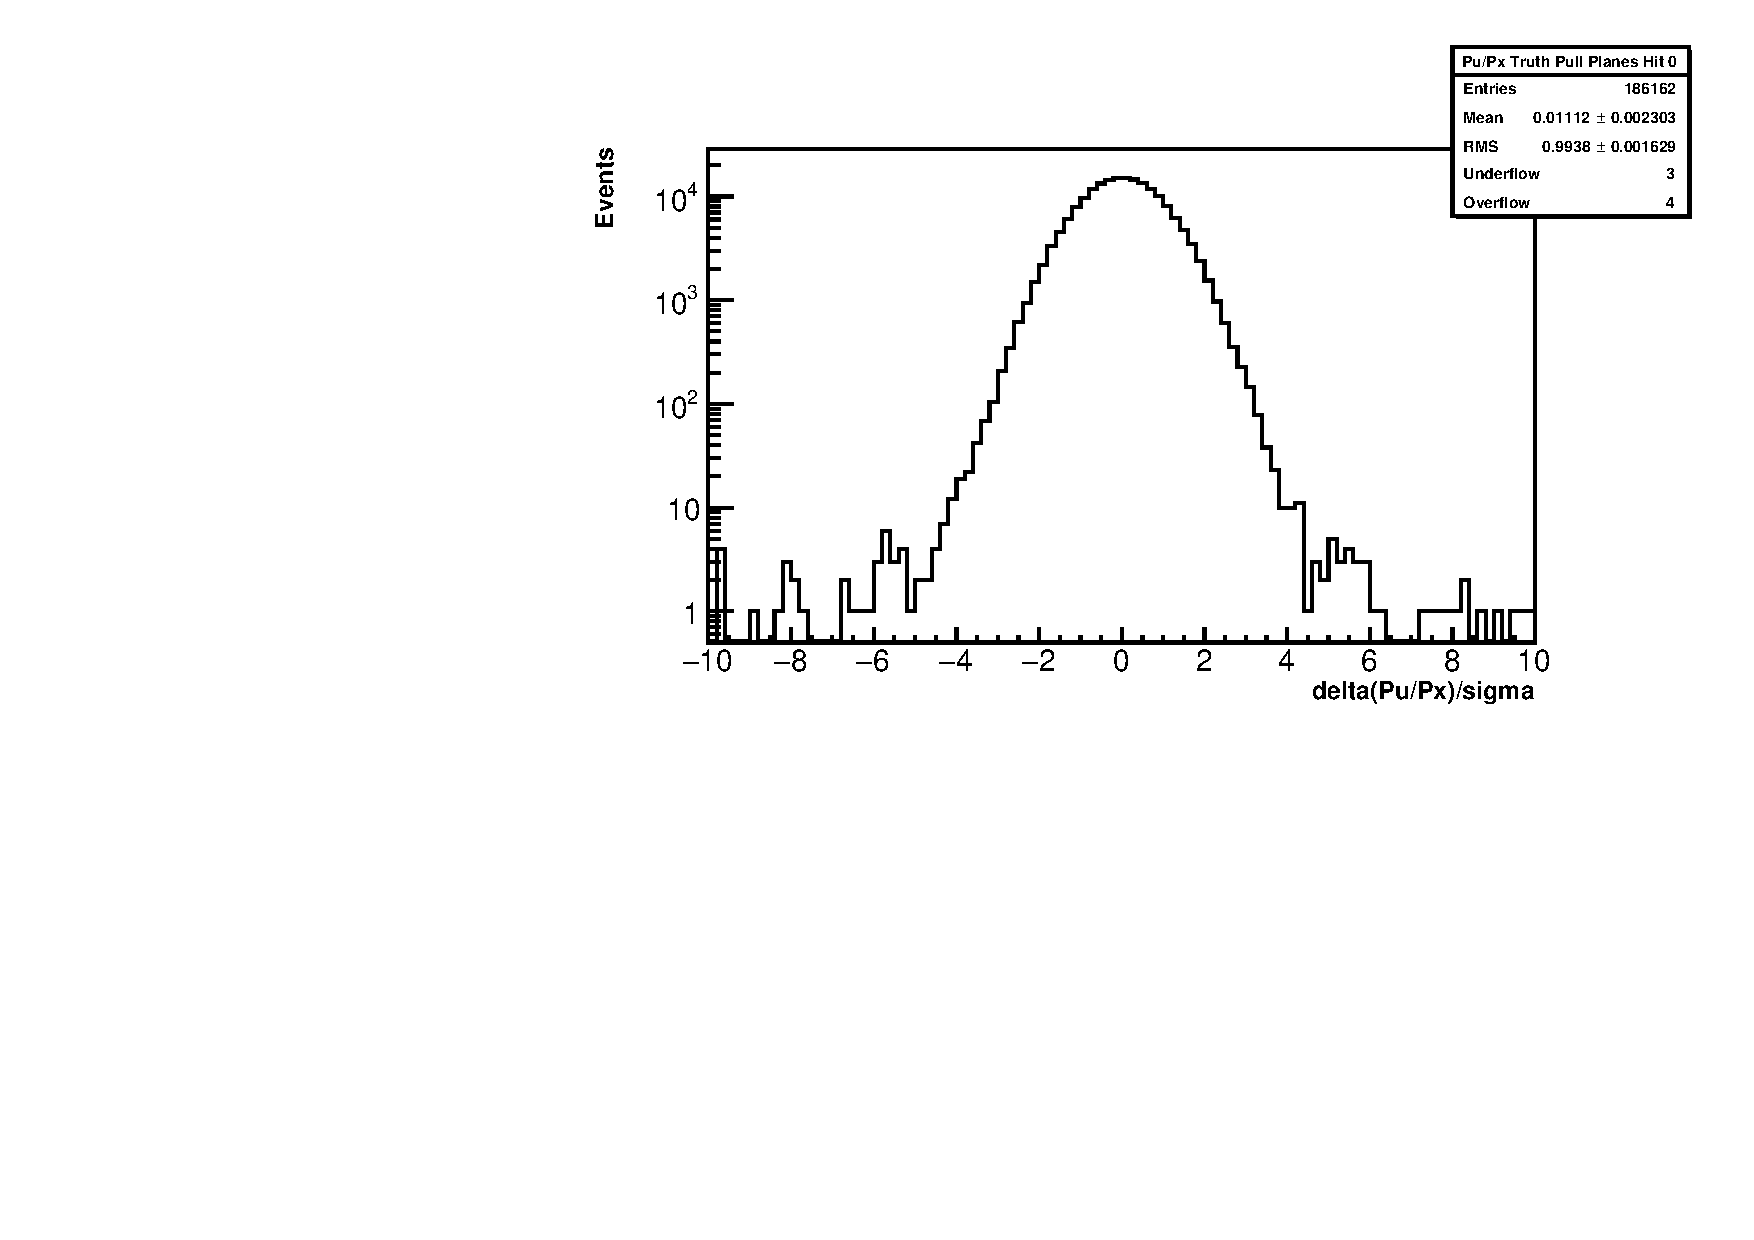
\includegraphics[width=1\textwidth]{PuPxpullLog} 
        \caption{Pu/Px truth pull on plane 0 for all tracks, log plot. Poor events can be seen as the distribution spreads out more towards the edges, with some under and overflows.}
    \end{subfigure}
    
    \begin{subfigure}[]{0.65\textwidth}
        \centering
        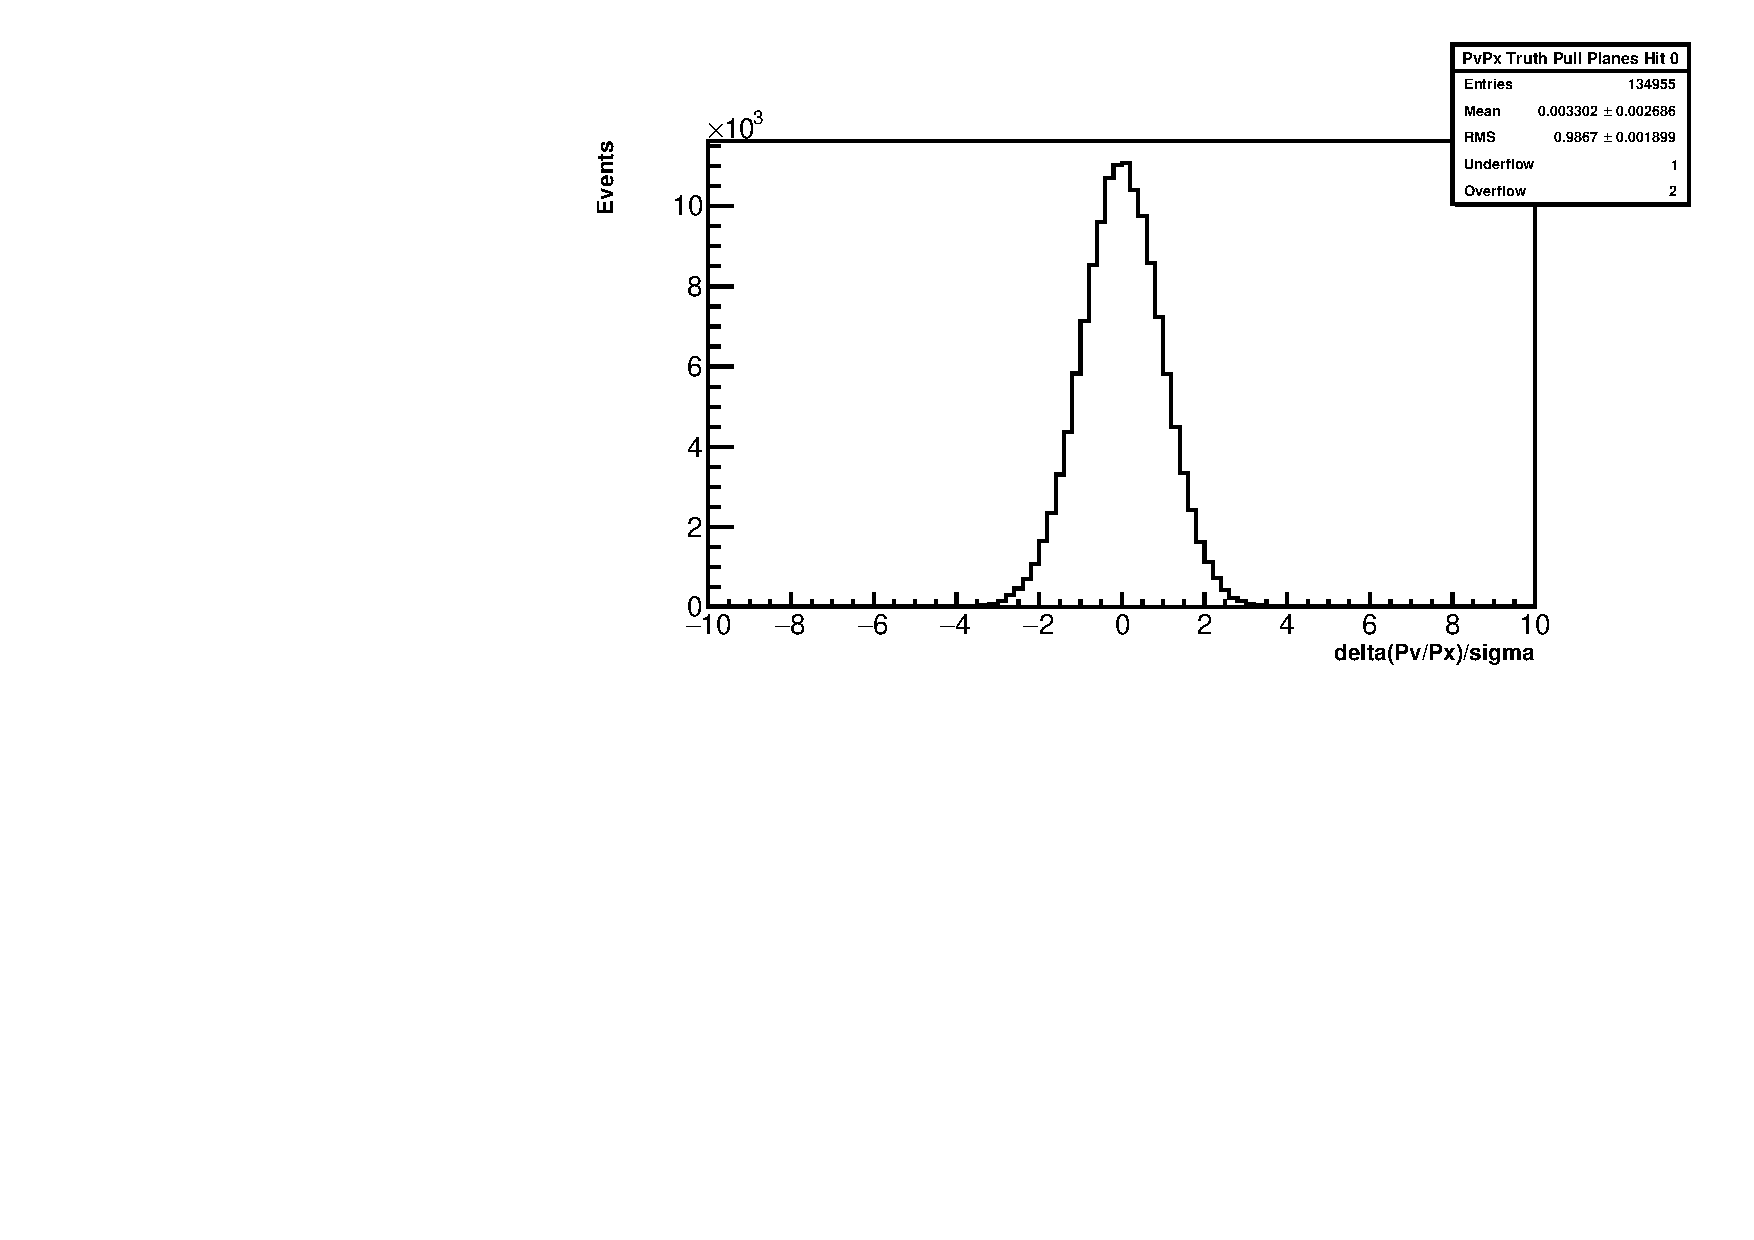
\includegraphics[width=1\textwidth]{PvPxpull} 
        \caption{Pv/Px truth pull on plane 0 for all tracks. Very close to a unit Gaussian showing the tracking is working correctly.}
    \end{subfigure}

    \begin{subfigure}[]{0.65\textwidth}
        \centering
        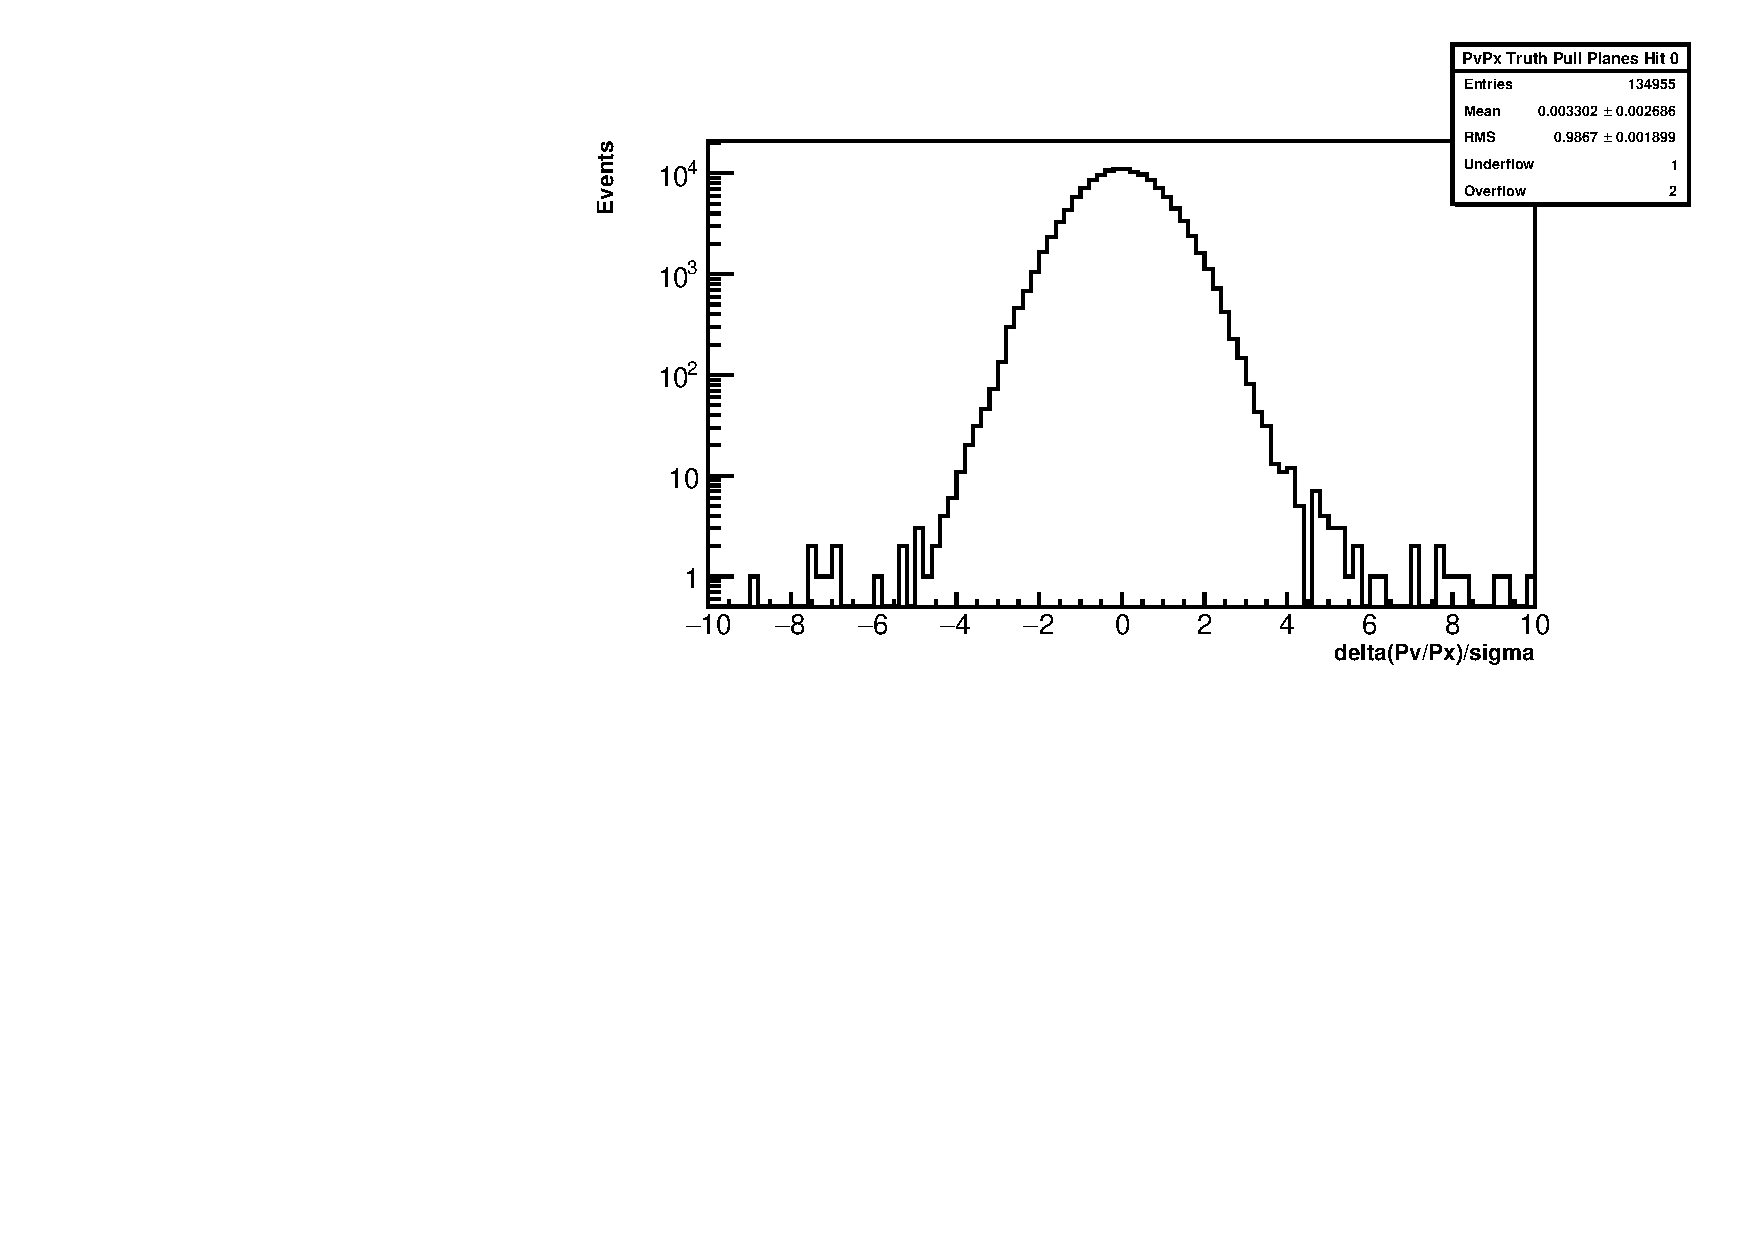
\includegraphics[width=1\textwidth]{PvPxpullLog} 
        \caption{Pv/Px truth pull on plane 0 for all tracks, log plot. Poor events can be seen as the distribution spreads out more towards the edges, with some under and overflows.}
    \end{subfigure}

    \caption{Truth pulls on plane 0 for all tracks.}
\end{figure}



\begin{figure}
    \centering
    \begin{subfigure}[]{0.8\textwidth}
        \centering
        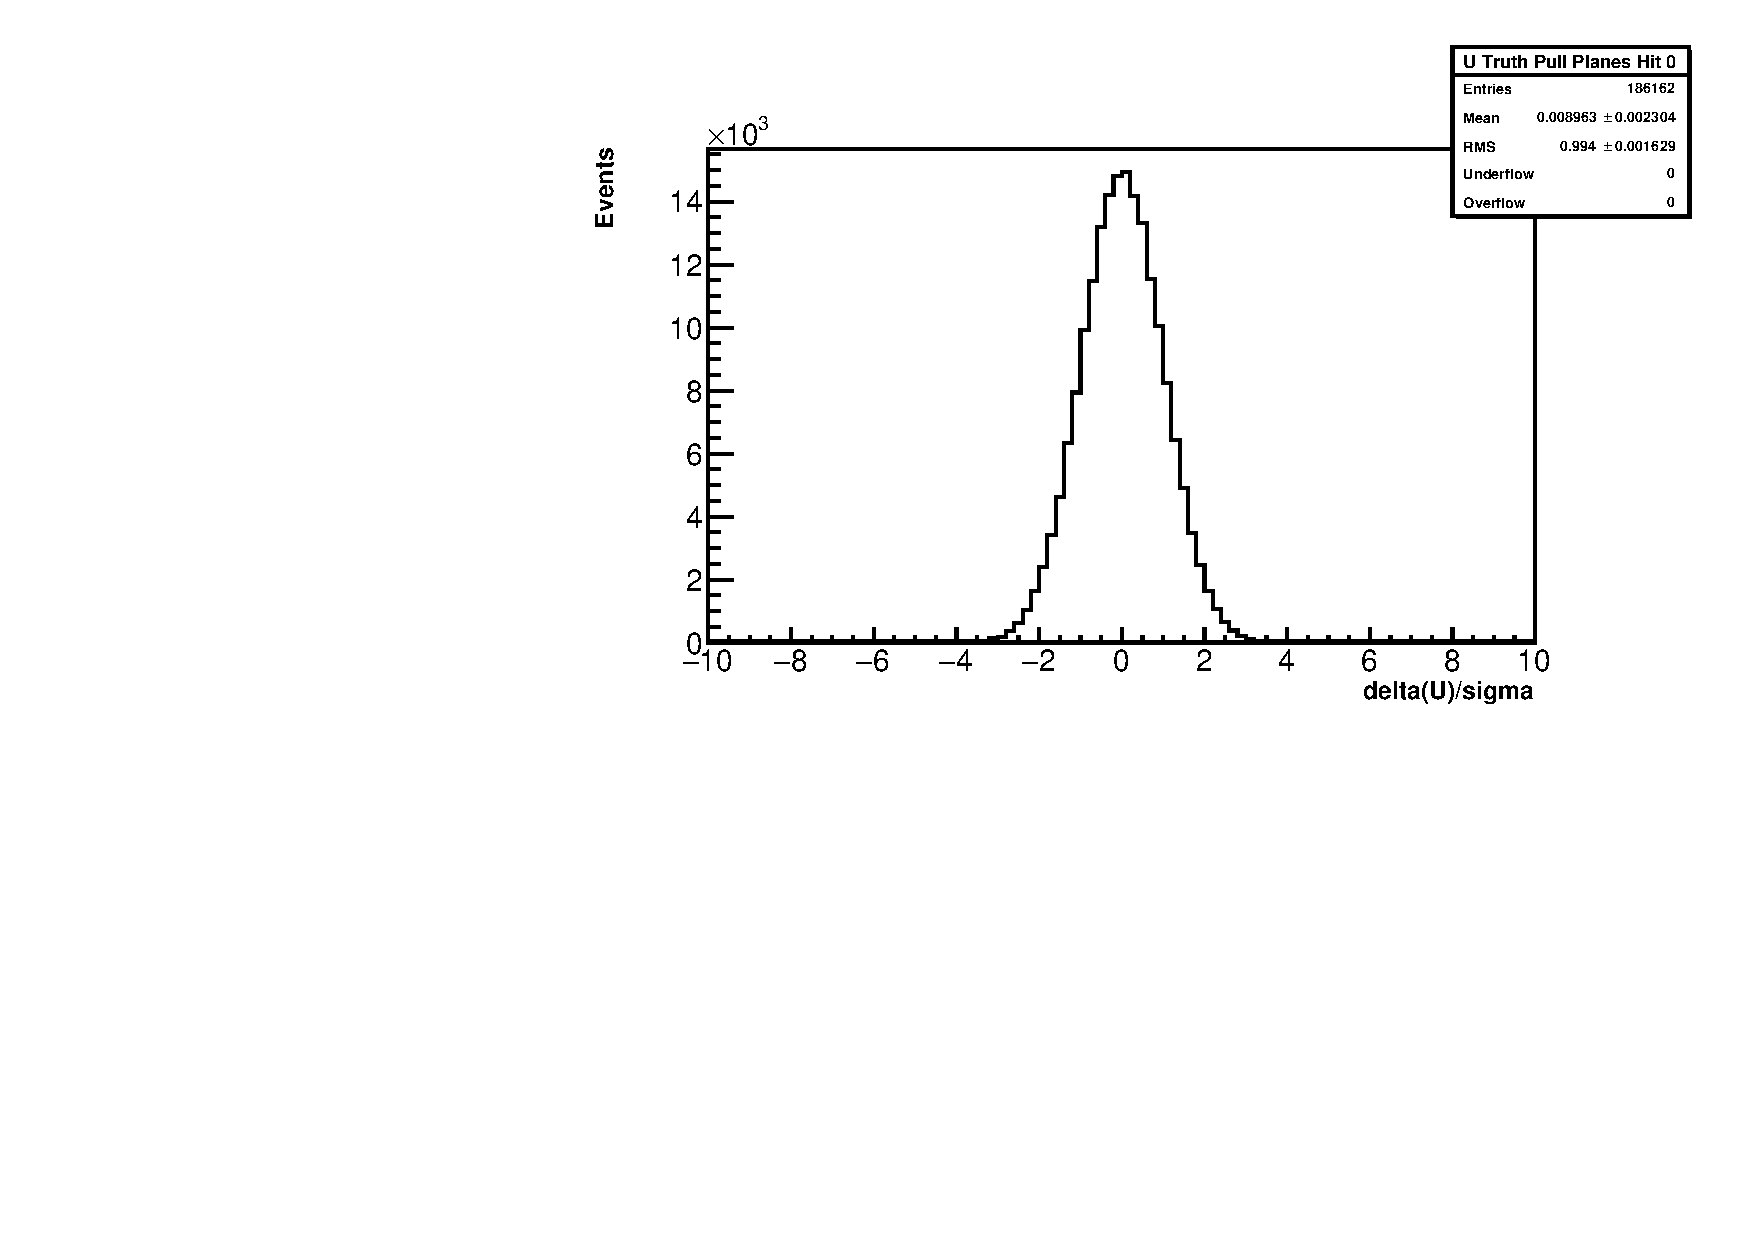
\includegraphics[width=1\textwidth]{Upull} 
        \caption{U truth pull on plane 0 for all tracks. Very close to a unit Gaussian showing the tracking is working correctly.}
    \end{subfigure}
    
    \begin{subfigure}[]{0.8\textwidth}
        \centering
        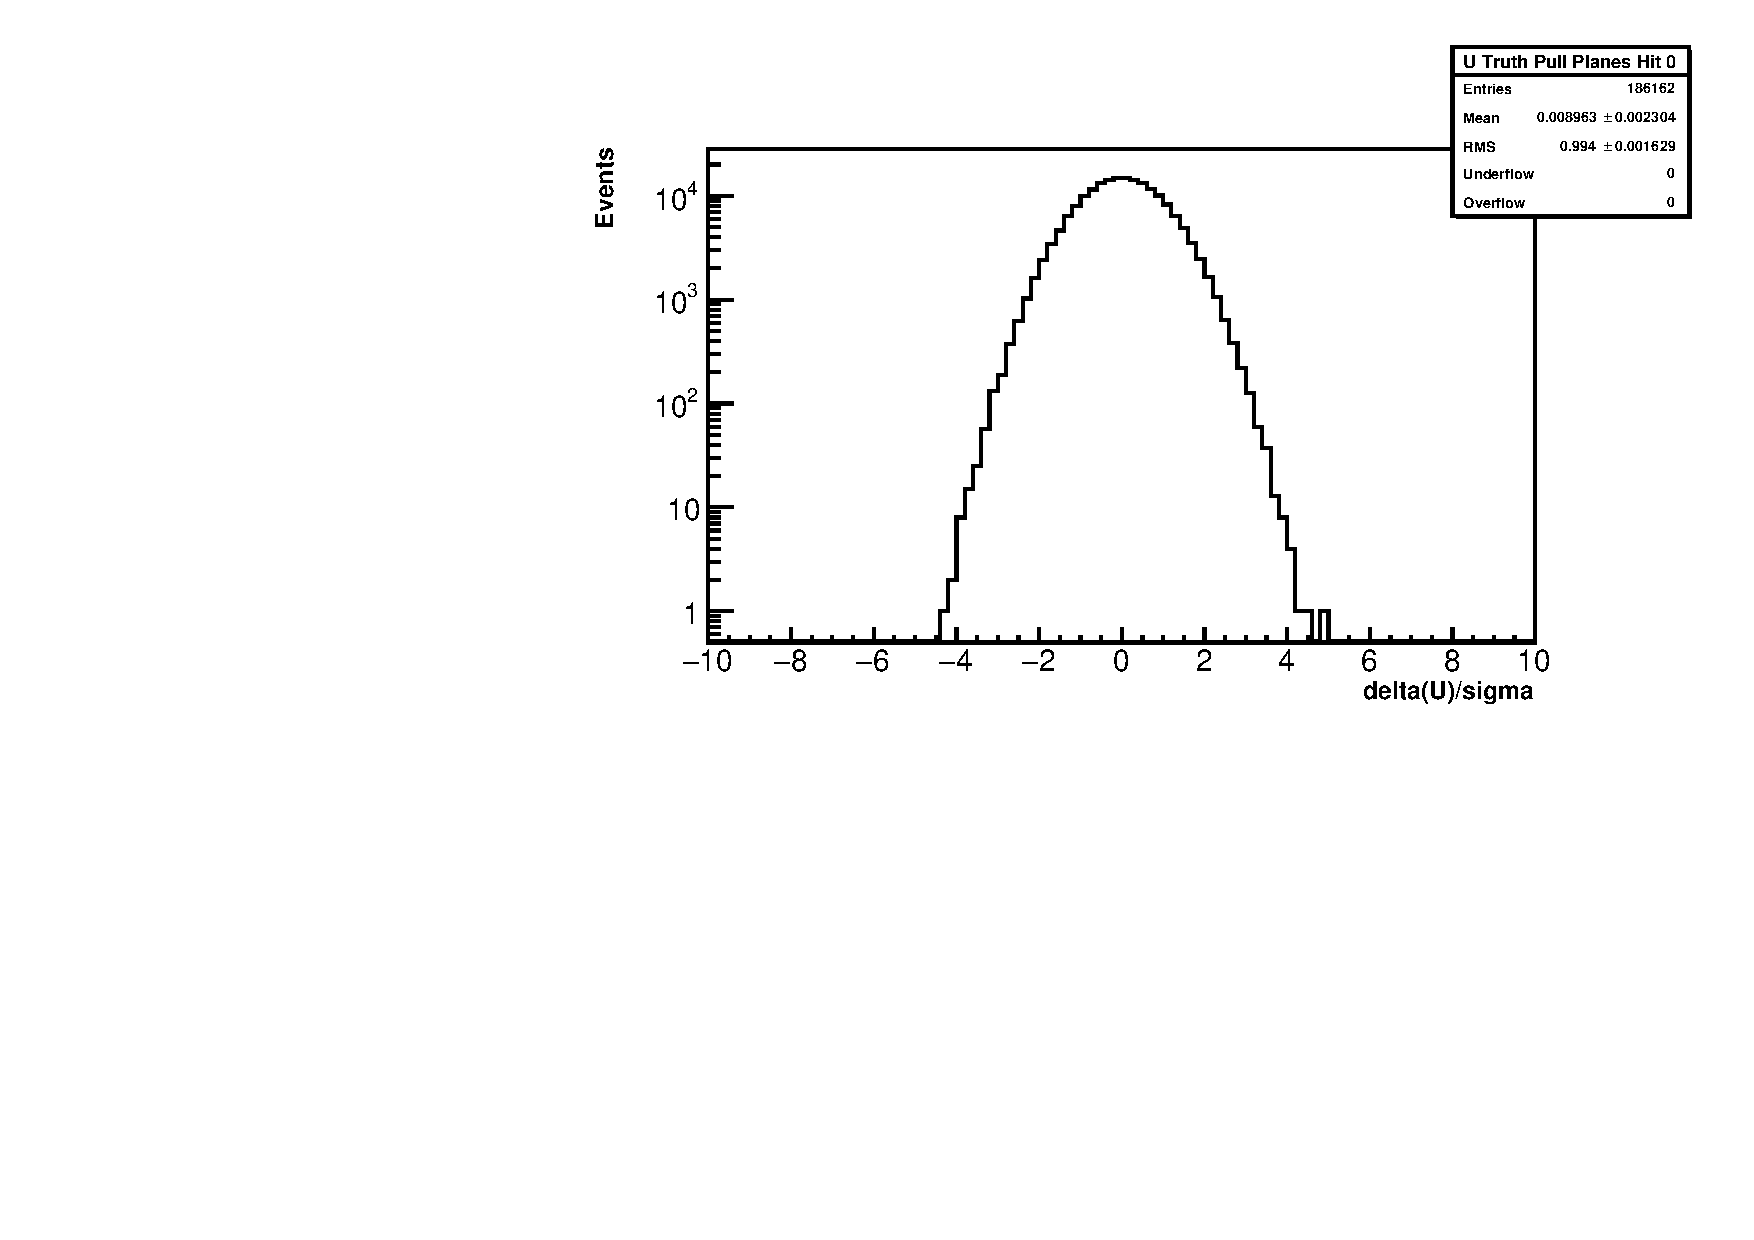
\includegraphics[width=1\textwidth]{UpullLog} 
        \caption{U truth pull on plane 0 for all tracks, log plot. Poor events can be seen as the distribution spreads out more towards the edges, with some under and overflows.}
    \end{subfigure}

    \caption{Number of iterations information.}
\end{figure}

\begin{figure}
    \centering
    \begin{subfigure}[]{0.8\textwidth}
        \centering
        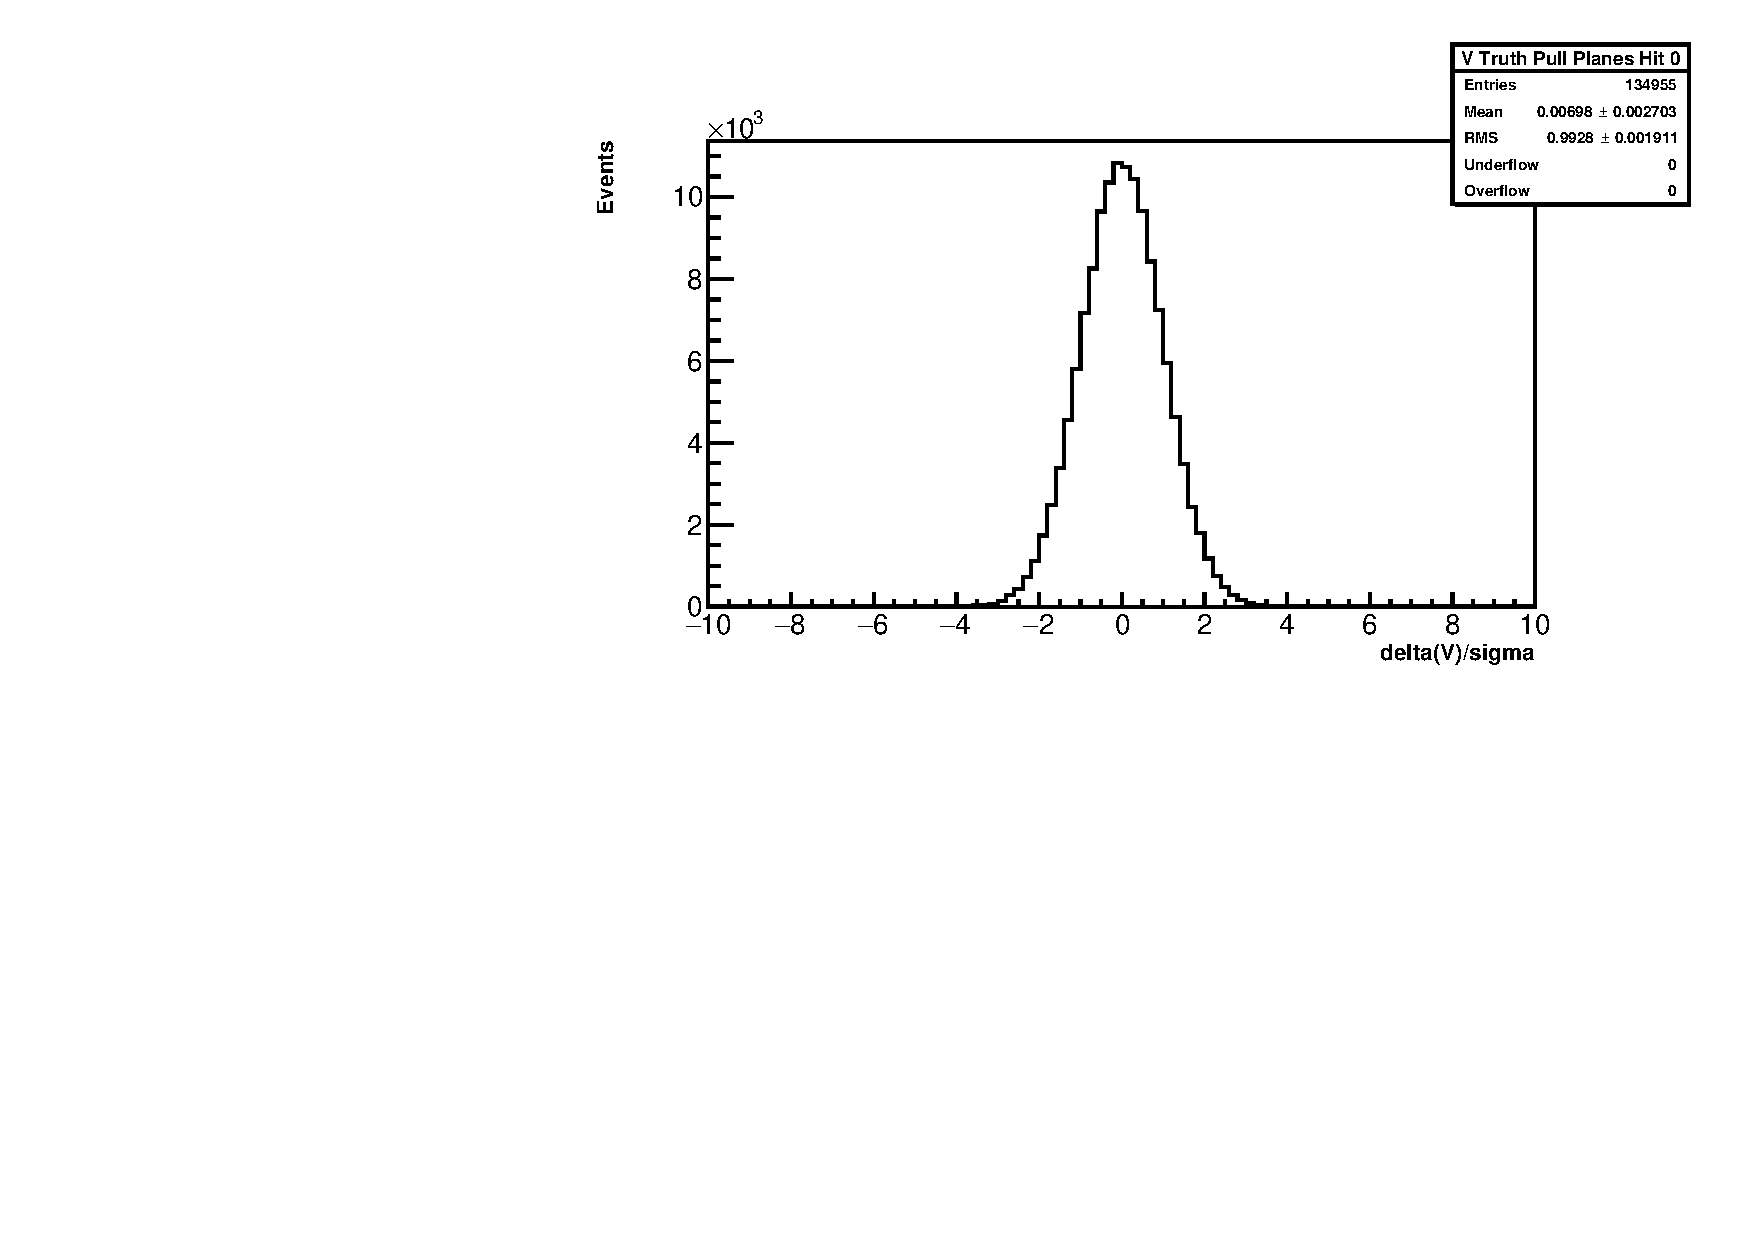
\includegraphics[width=1\textwidth]{Vpull} 
        \caption{V truth pull on plane 0 for all tracks. Very close to a unit Gaussian showing the tracking is working correctly.}
    \end{subfigure}
    
    \begin{subfigure}[]{0.8\textwidth}
        \centering
        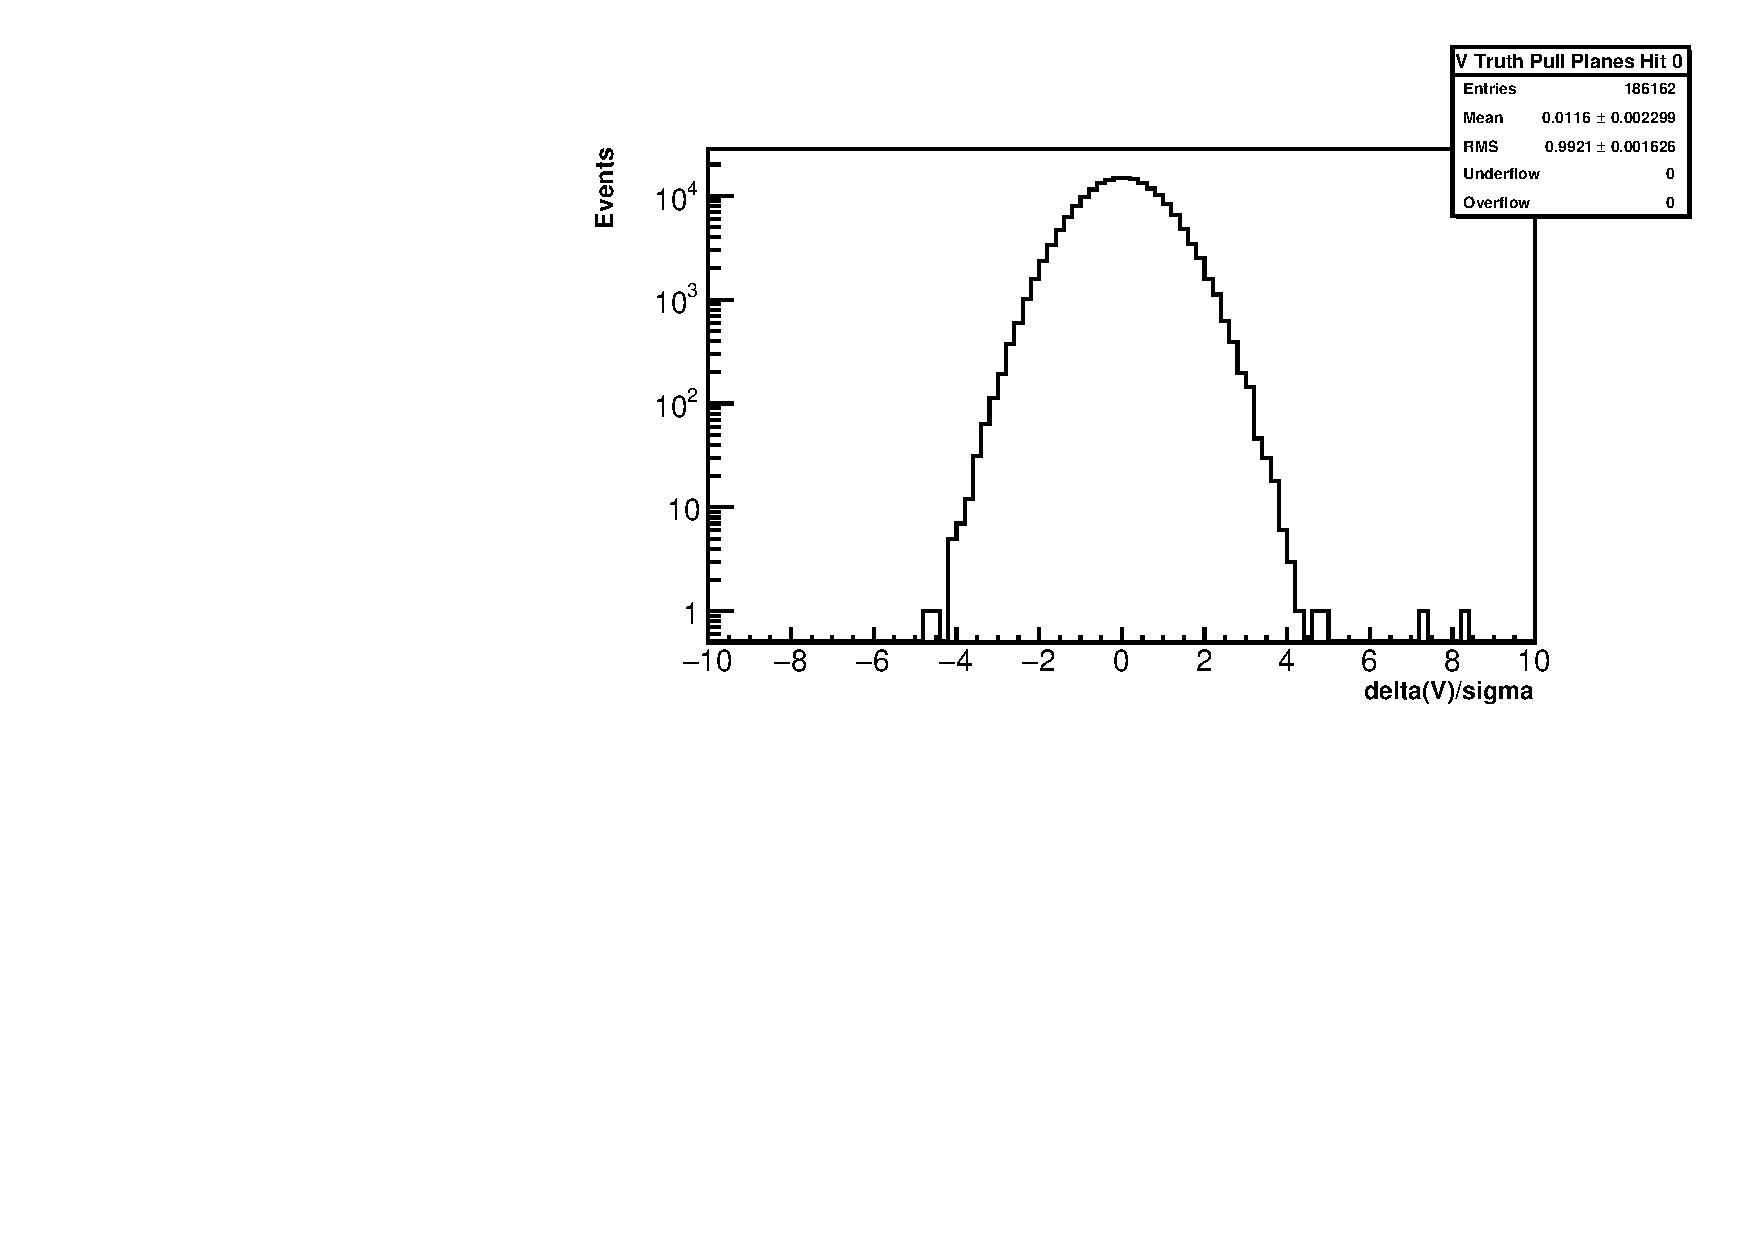
\includegraphics[width=1\textwidth]{VpullLog} 
        \caption{V truth pull on plane 0 for all tracks, log plot. Poor events can be seen as the distribution spreads out more towards the edges, with some under and overflows.}
    \end{subfigure}

    \caption{Number of iterations information.}
\end{figure}



\begin{figure}
    \centering
    \begin{subfigure}[]{0.6\textwidth}
        \centering
        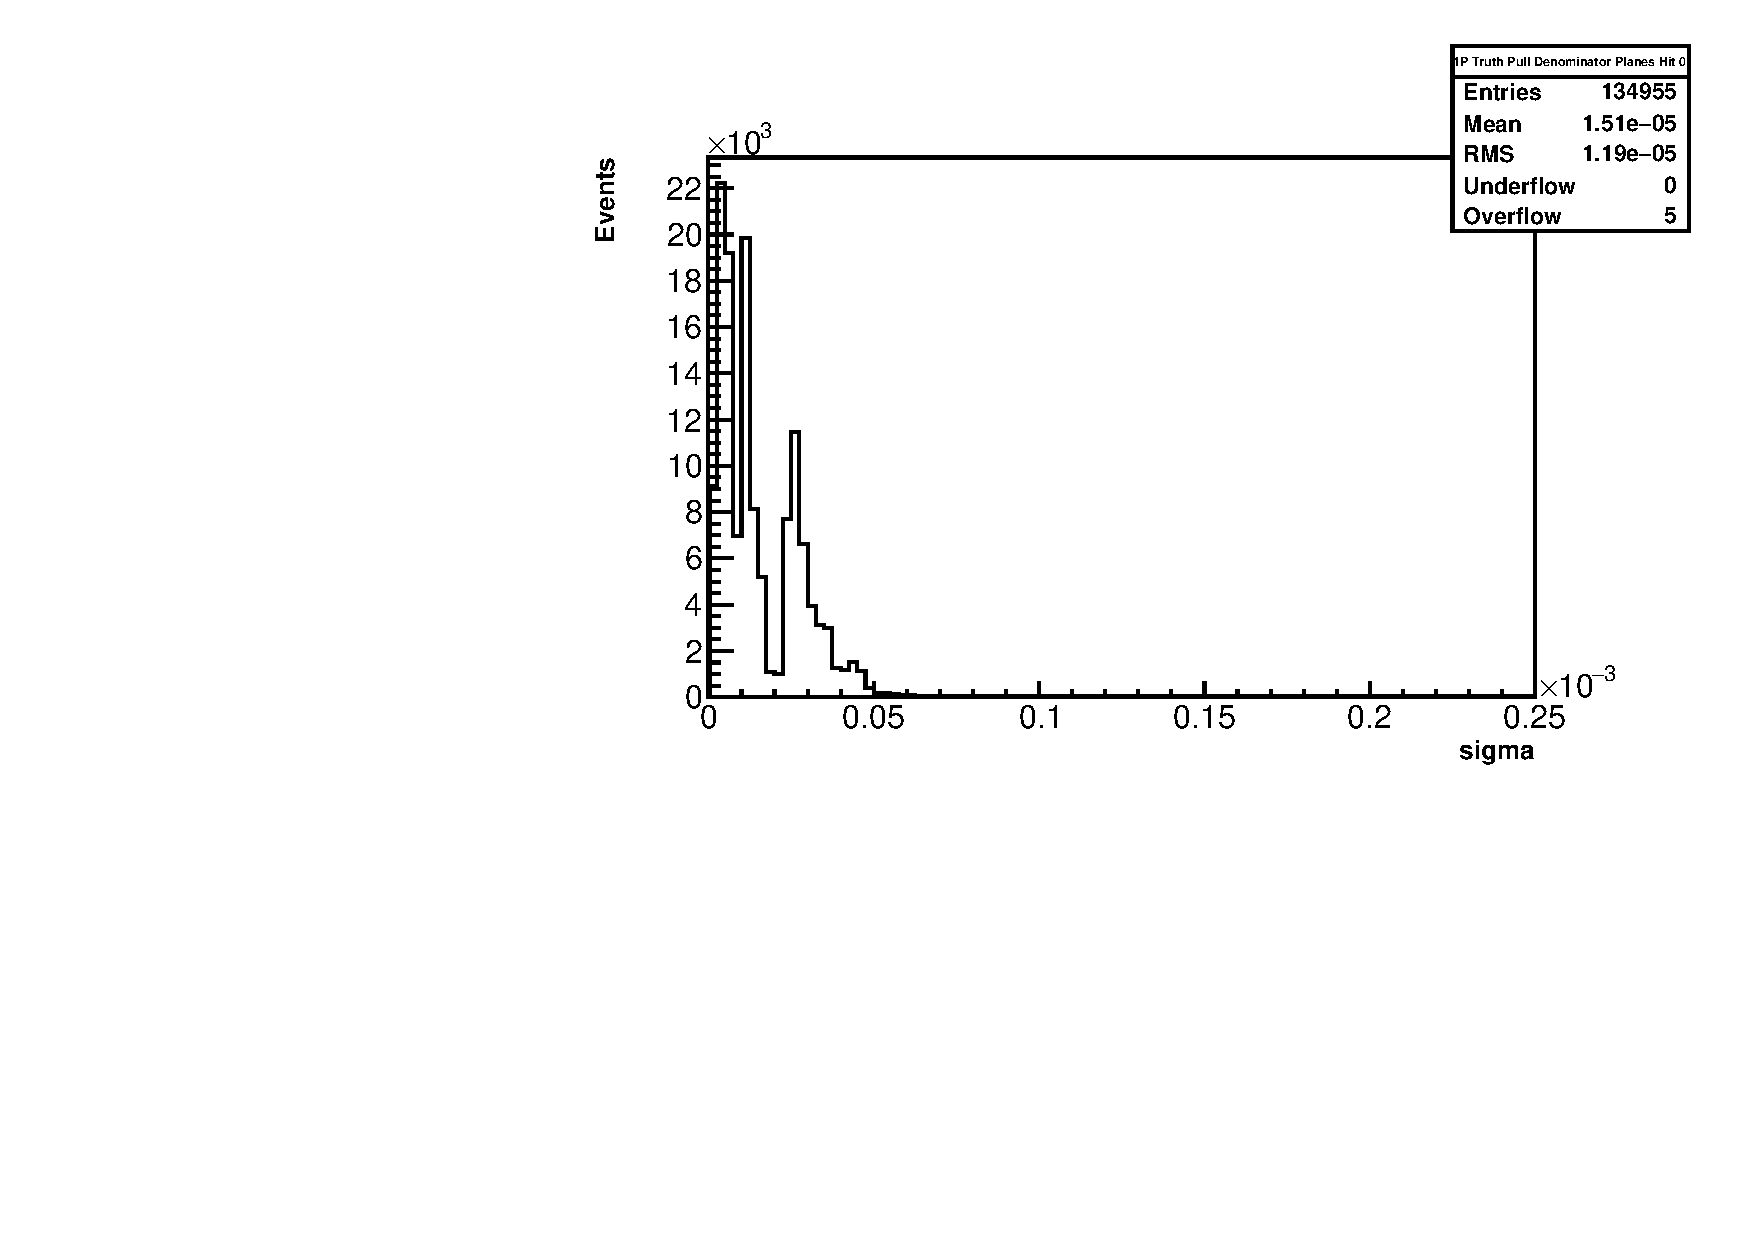
\includegraphics[width=1\textwidth]{1PpullDenom} 
        \caption{The error (denominator), in the 1/P pull. The different spikes corresponds to different numbers of planes hit, or different amounts of material passed through.}
    \end{subfigure}

    \begin{subfigure}[]{0.6\textwidth}
        \centering
        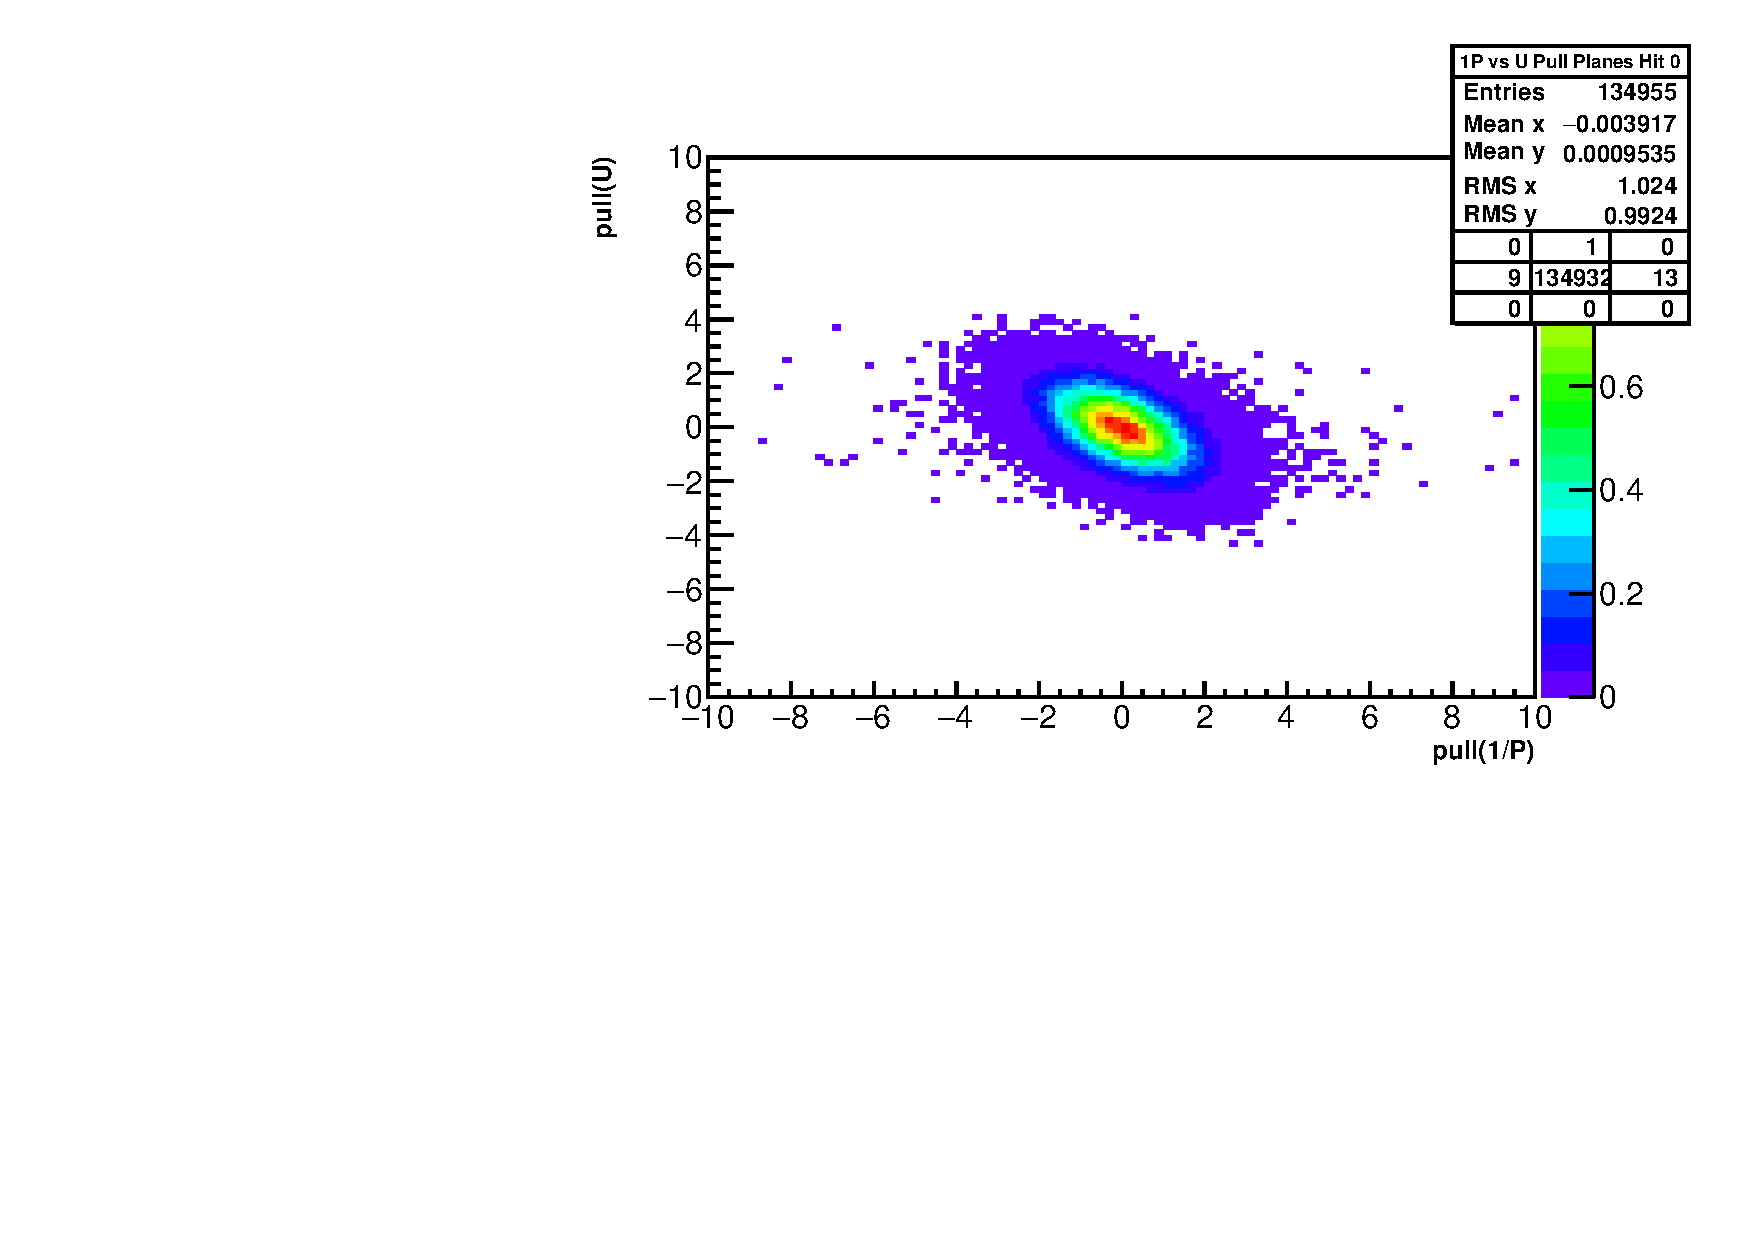
\includegraphics[width=1\textwidth]{1PpullVsUpull} 
        \caption{1/P pull vs U pull, the poor events can be seen spreading in a non-uniform way from the target.}
    \end{subfigure}
    
    \begin{subfigure}[]{0.6\textwidth}
        \centering
        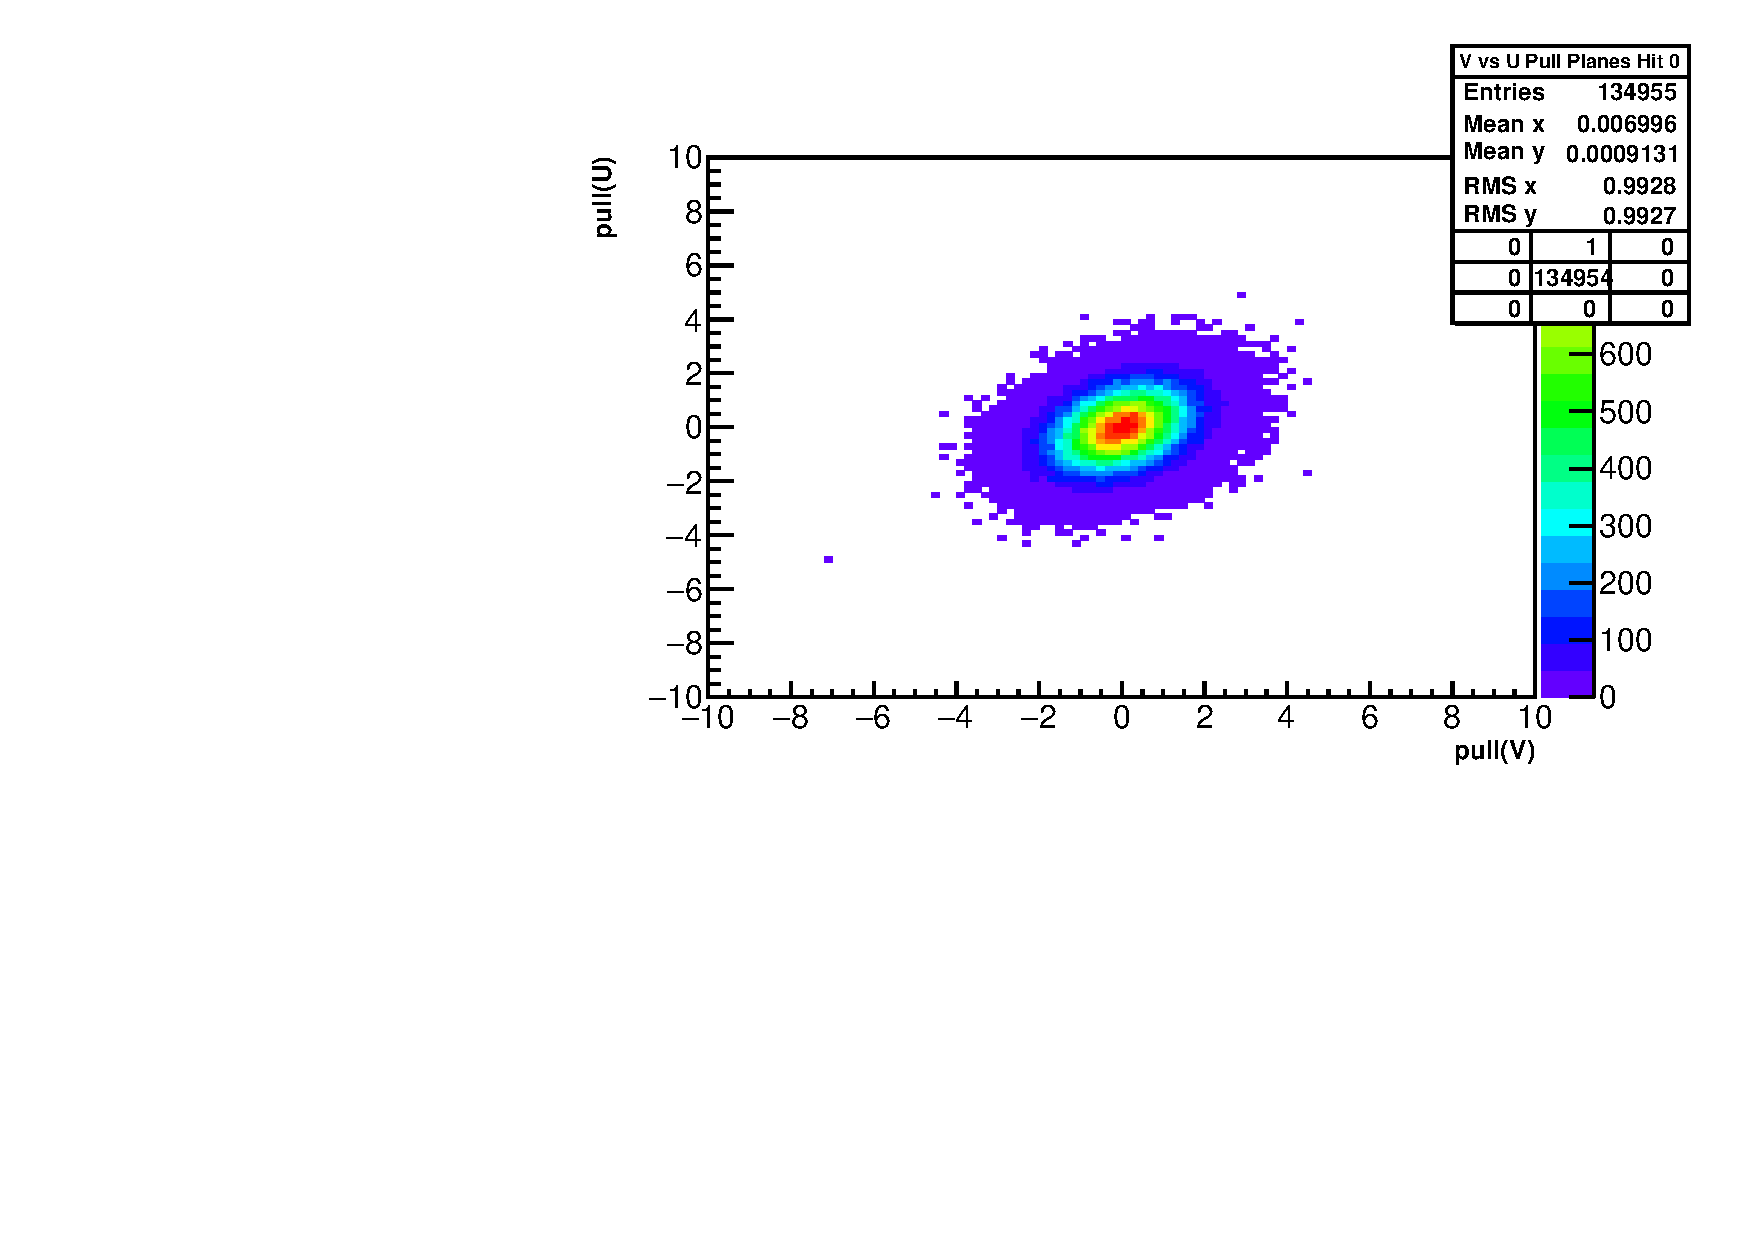
\includegraphics[width=1\textwidth]{UpullVsVpull} 
        \caption{U pull vs V pull.}
    \end{subfigure}

    \caption{Some various pull related plots.}
\end{figure}


\begin{figure}
    \centering
    \begin{subfigure}[]{0.6\textwidth}
        \centering
        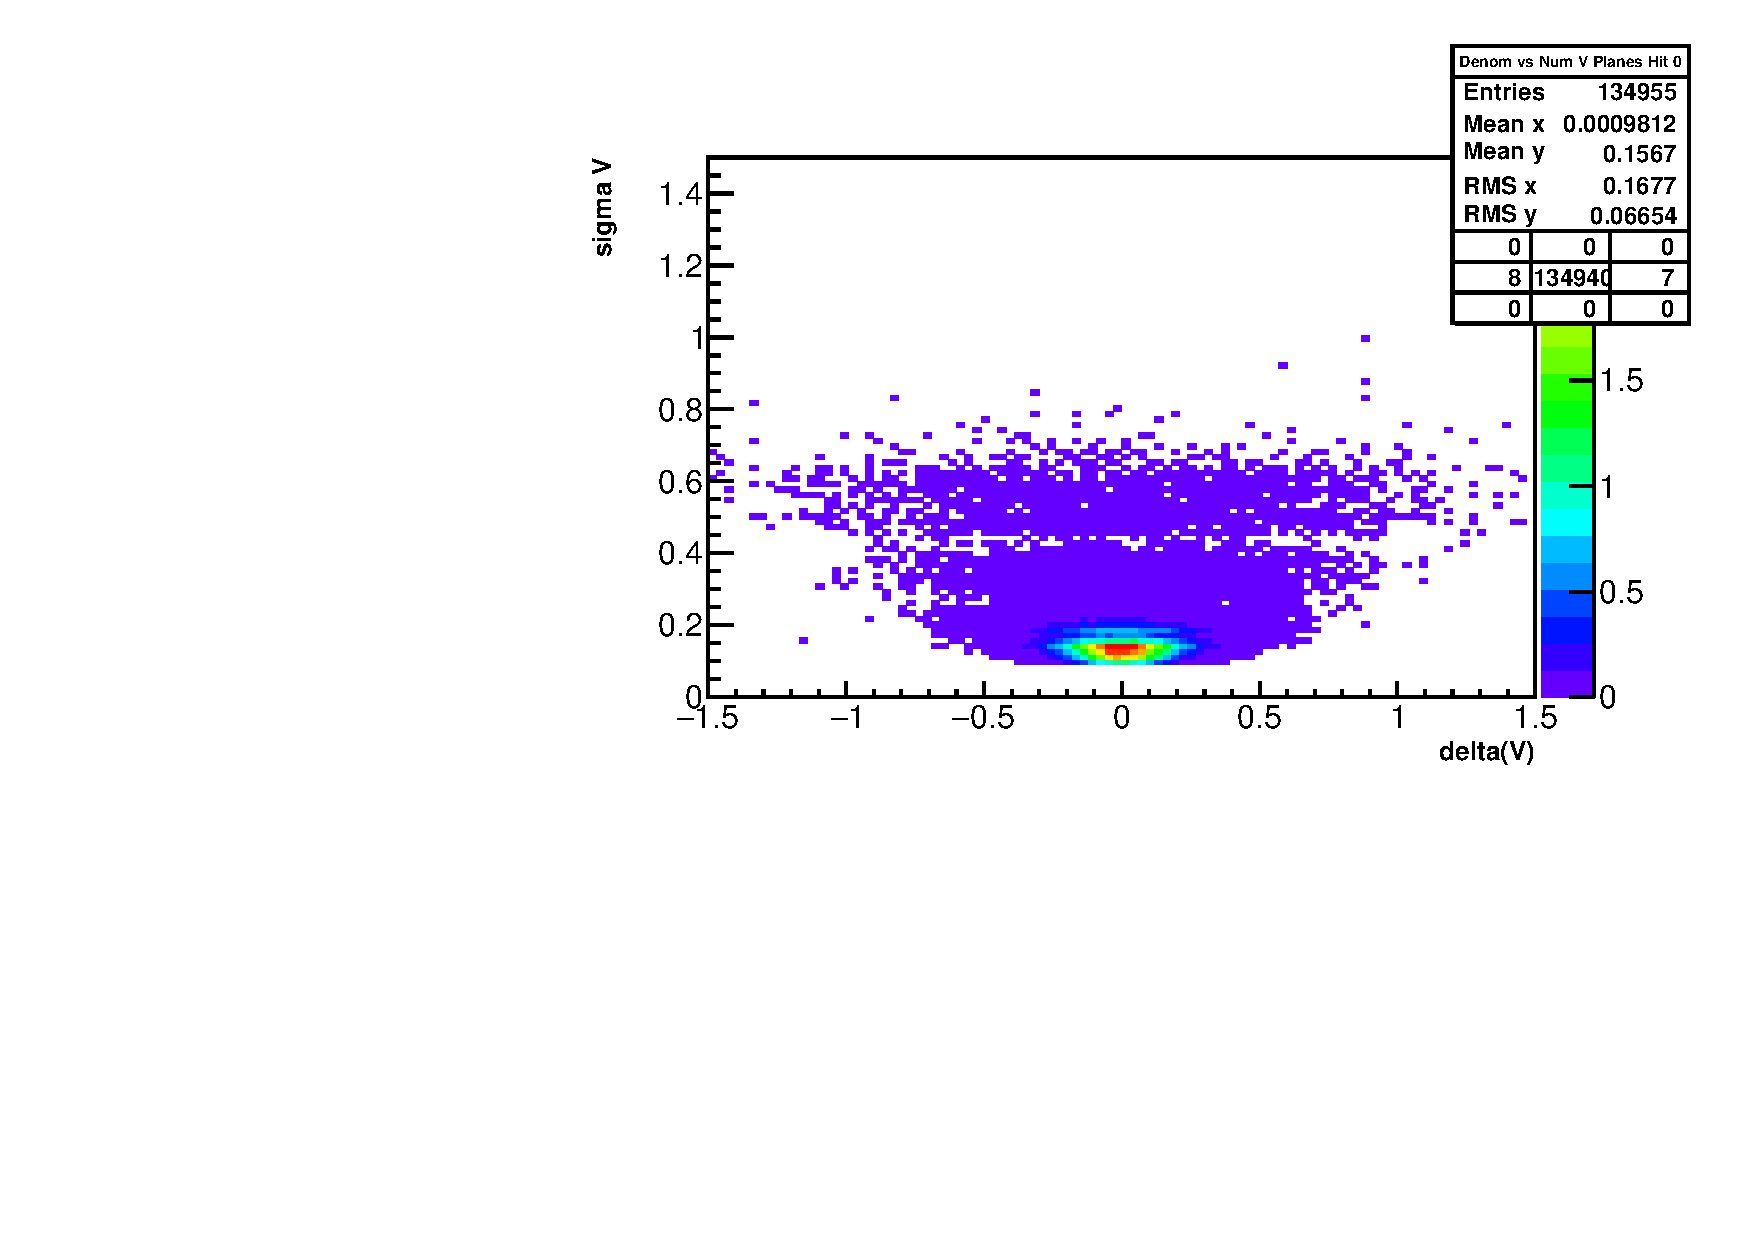
\includegraphics[width=1\textwidth]{VpullNumDenom} 
        \caption{The error in the V pull vs the residual in the V pull. The upper events are mostly comprised of tracks which hit less planes, leading to larger errors.}
    \end{subfigure}

    \begin{subfigure}[]{0.6\textwidth}
        \centering
        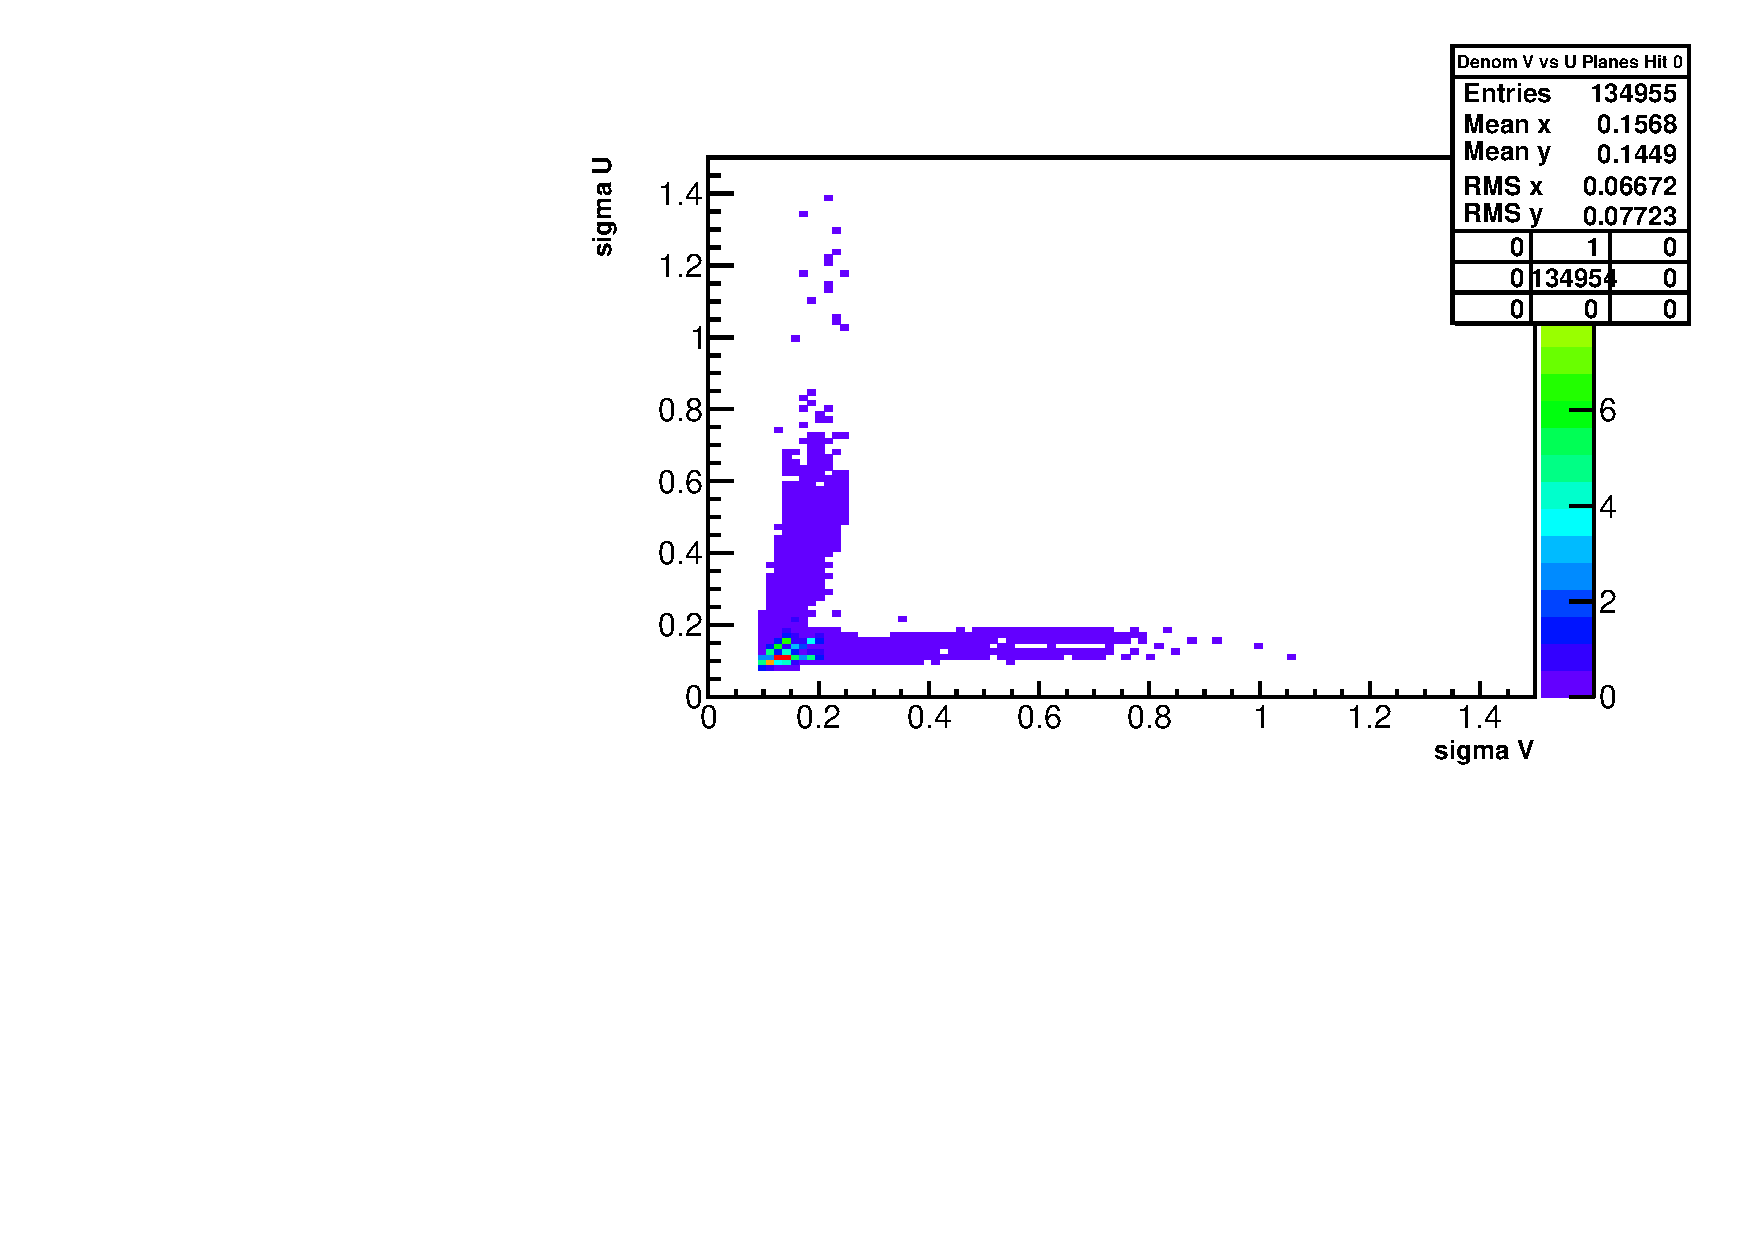
\includegraphics[width=1\textwidth]{DenomUV} 
        \caption{Error in U pull vs error in V pull, can be seen to be mostly uncorrelated within the fit.}
    \end{subfigure}
    
    \begin{subfigure}[]{0.6\textwidth}
        \centering
        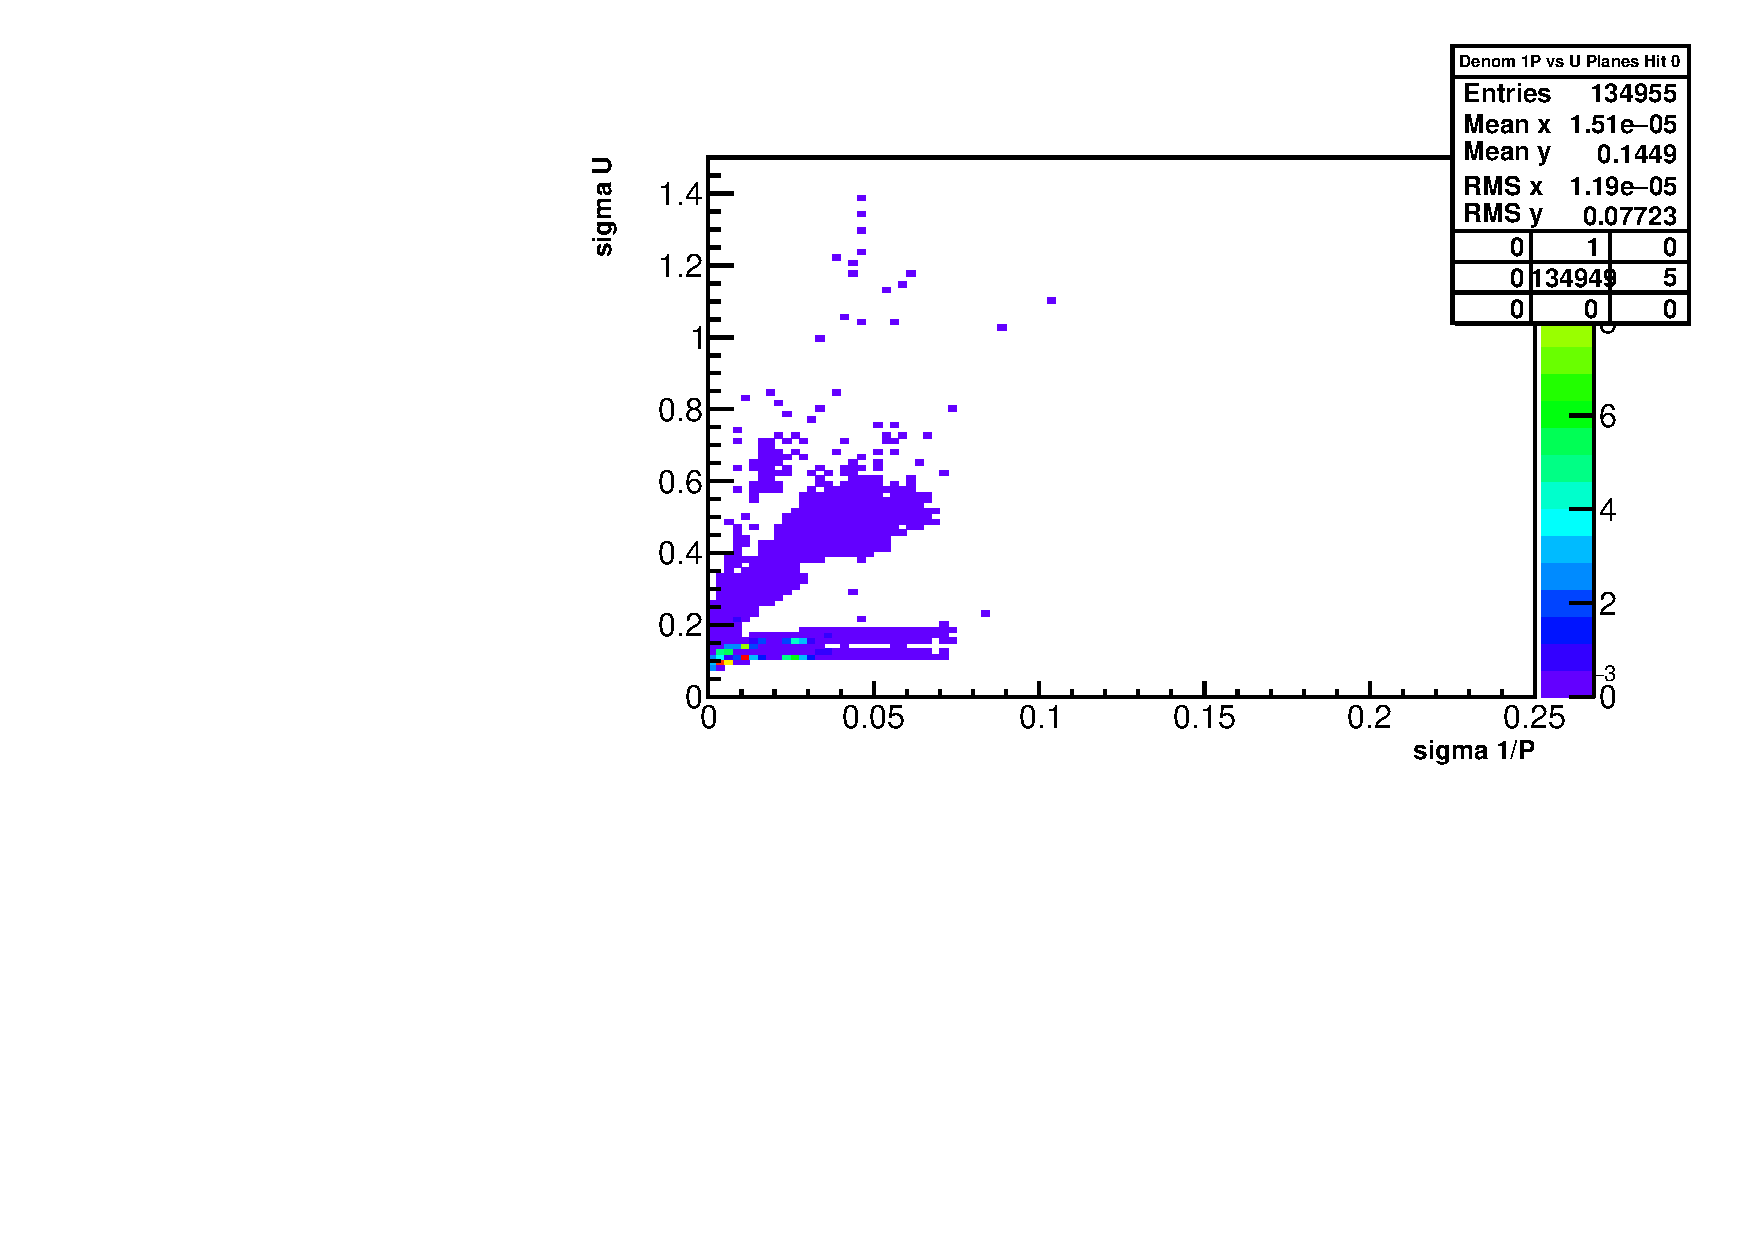
\includegraphics[width=1\textwidth]{Denom1PU} 
        \caption{Error in U pull vs error in 1/P pull. Some interesting structure is observed, that is not fully understood.}
    \end{subfigure}

    \caption{Some various pull related plots.}
\end{figure}



\begin{figure}
    \centering
    \begin{subfigure}[]{0.5\textwidth}
        \centering
        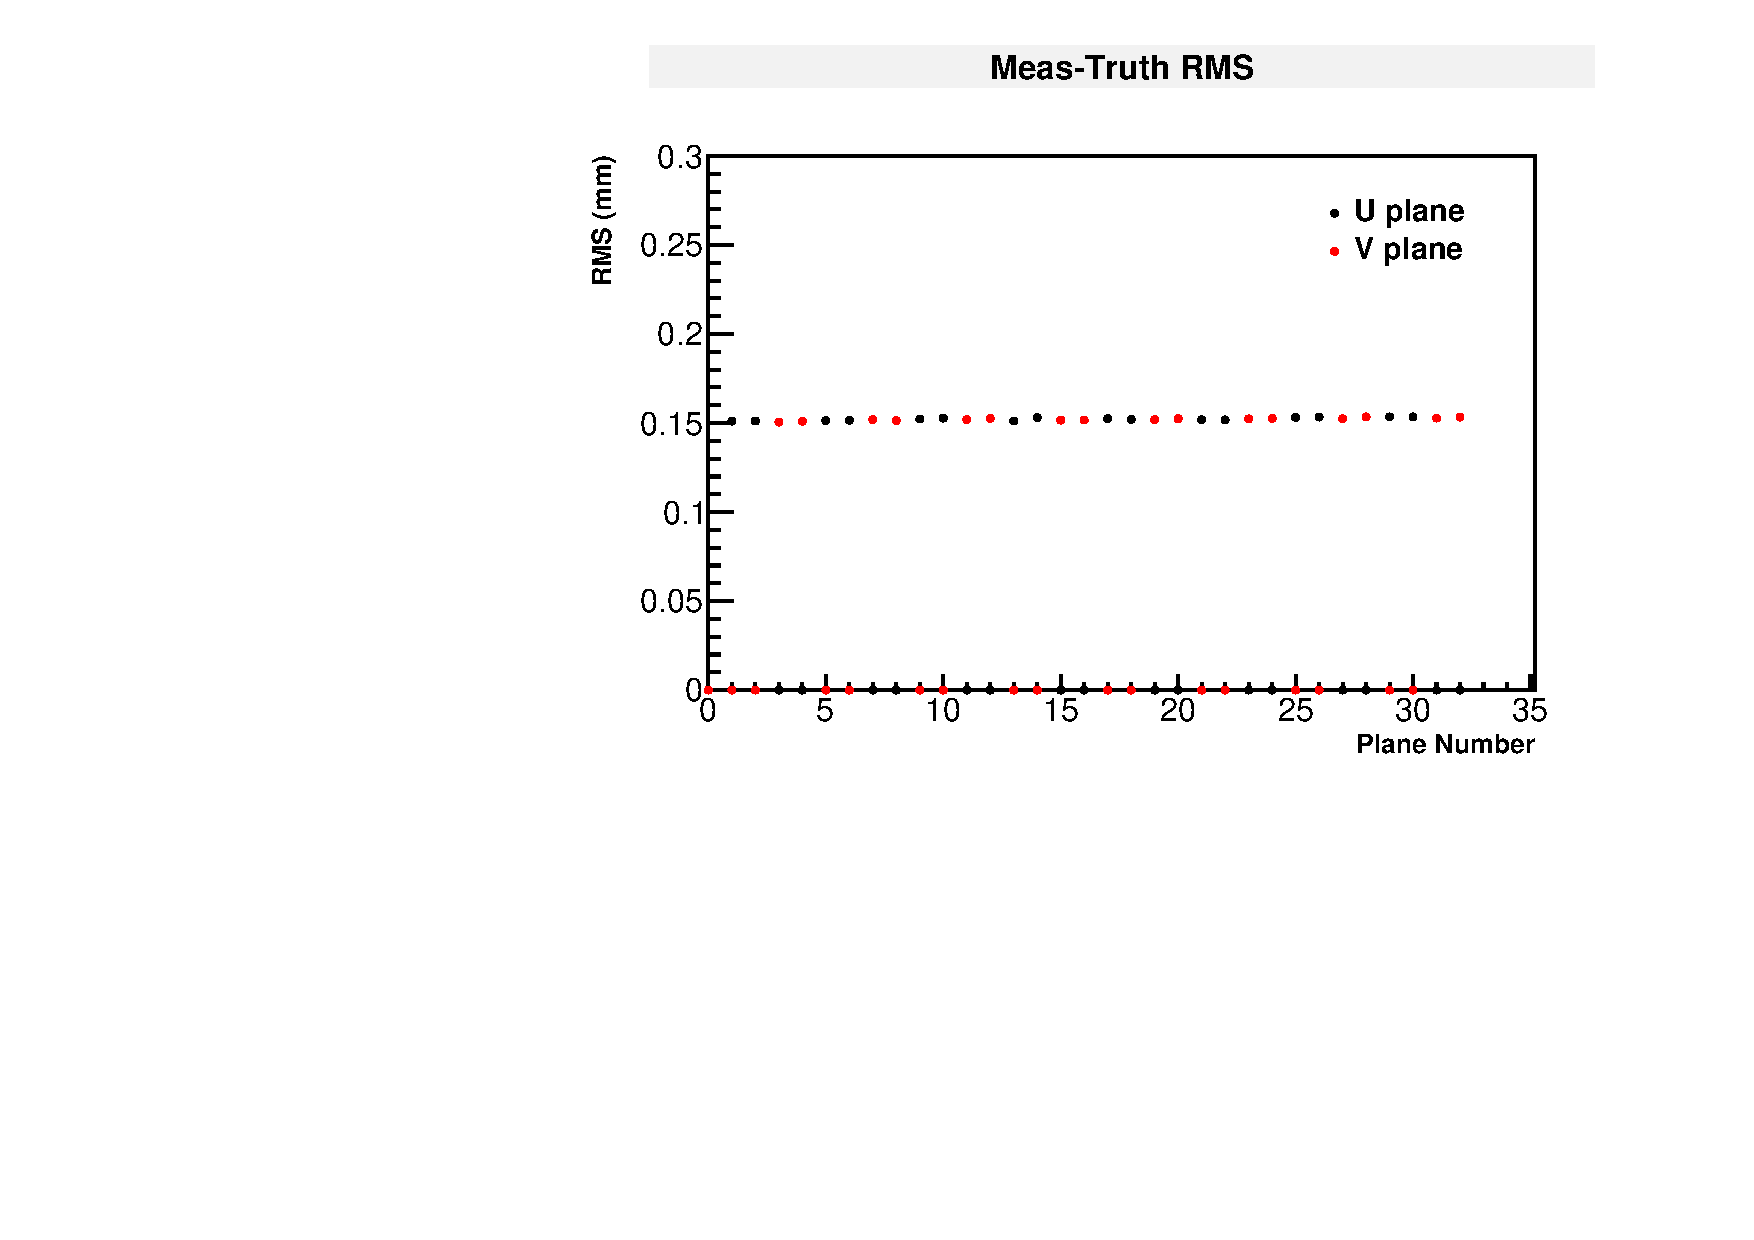
\includegraphics[width=1\textwidth]{meastruthrms} 
        \caption{RMS of measured - truth residuals, the input 150 $\mu$m smearing can be seen. Points on the X axis signify no measurement of that parameter on that plane.}
    \end{subfigure}

    \begin{subfigure}[]{0.5\textwidth}
        \centering
        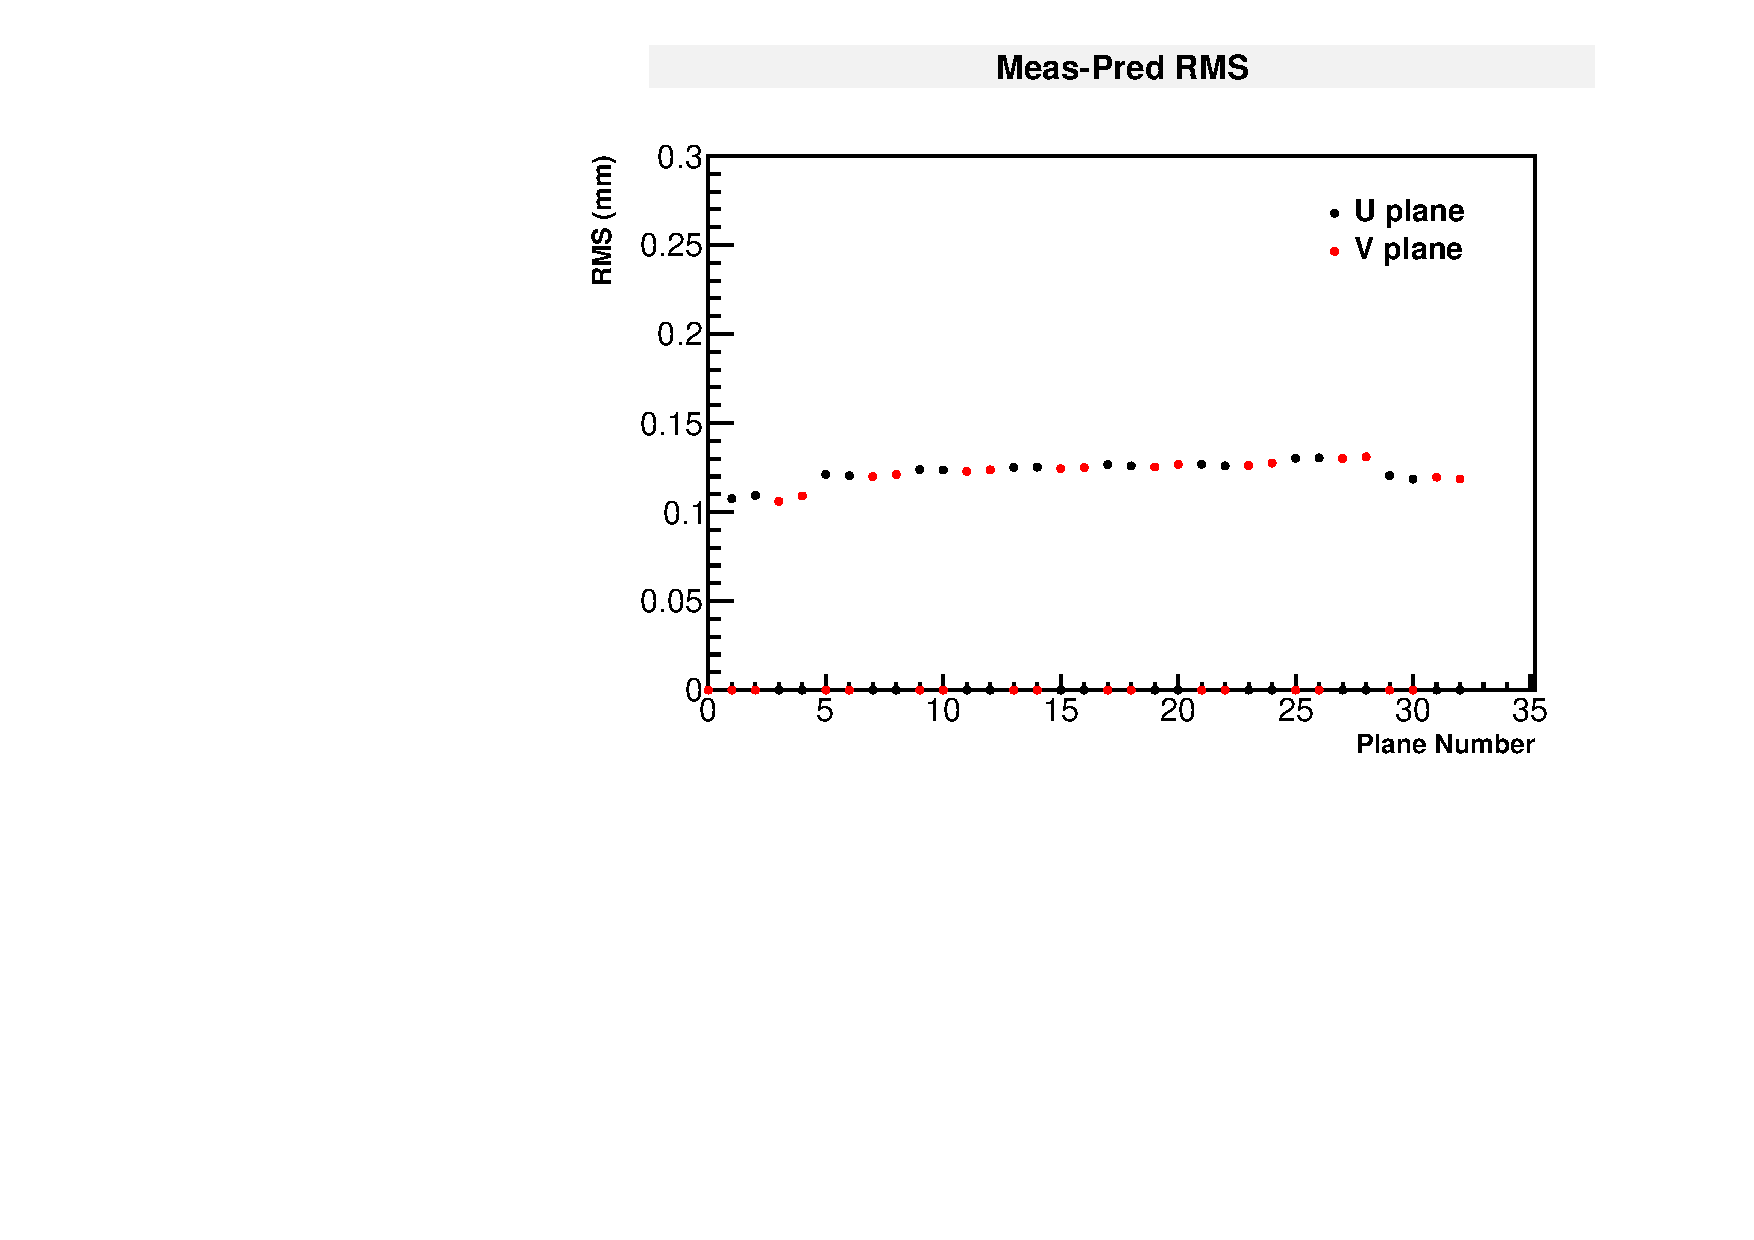
\includegraphics[width=1\textwidth]{measpredrms} 
        \caption{RMS of measured - predicted residuals. There is an overall upside down parabolic shape to the distribution. A slight rise towards higher plane number indicates larger error due to increased material.}
    \end{subfigure}
    
    \begin{subfigure}[]{0.5\textwidth}
        \centering
        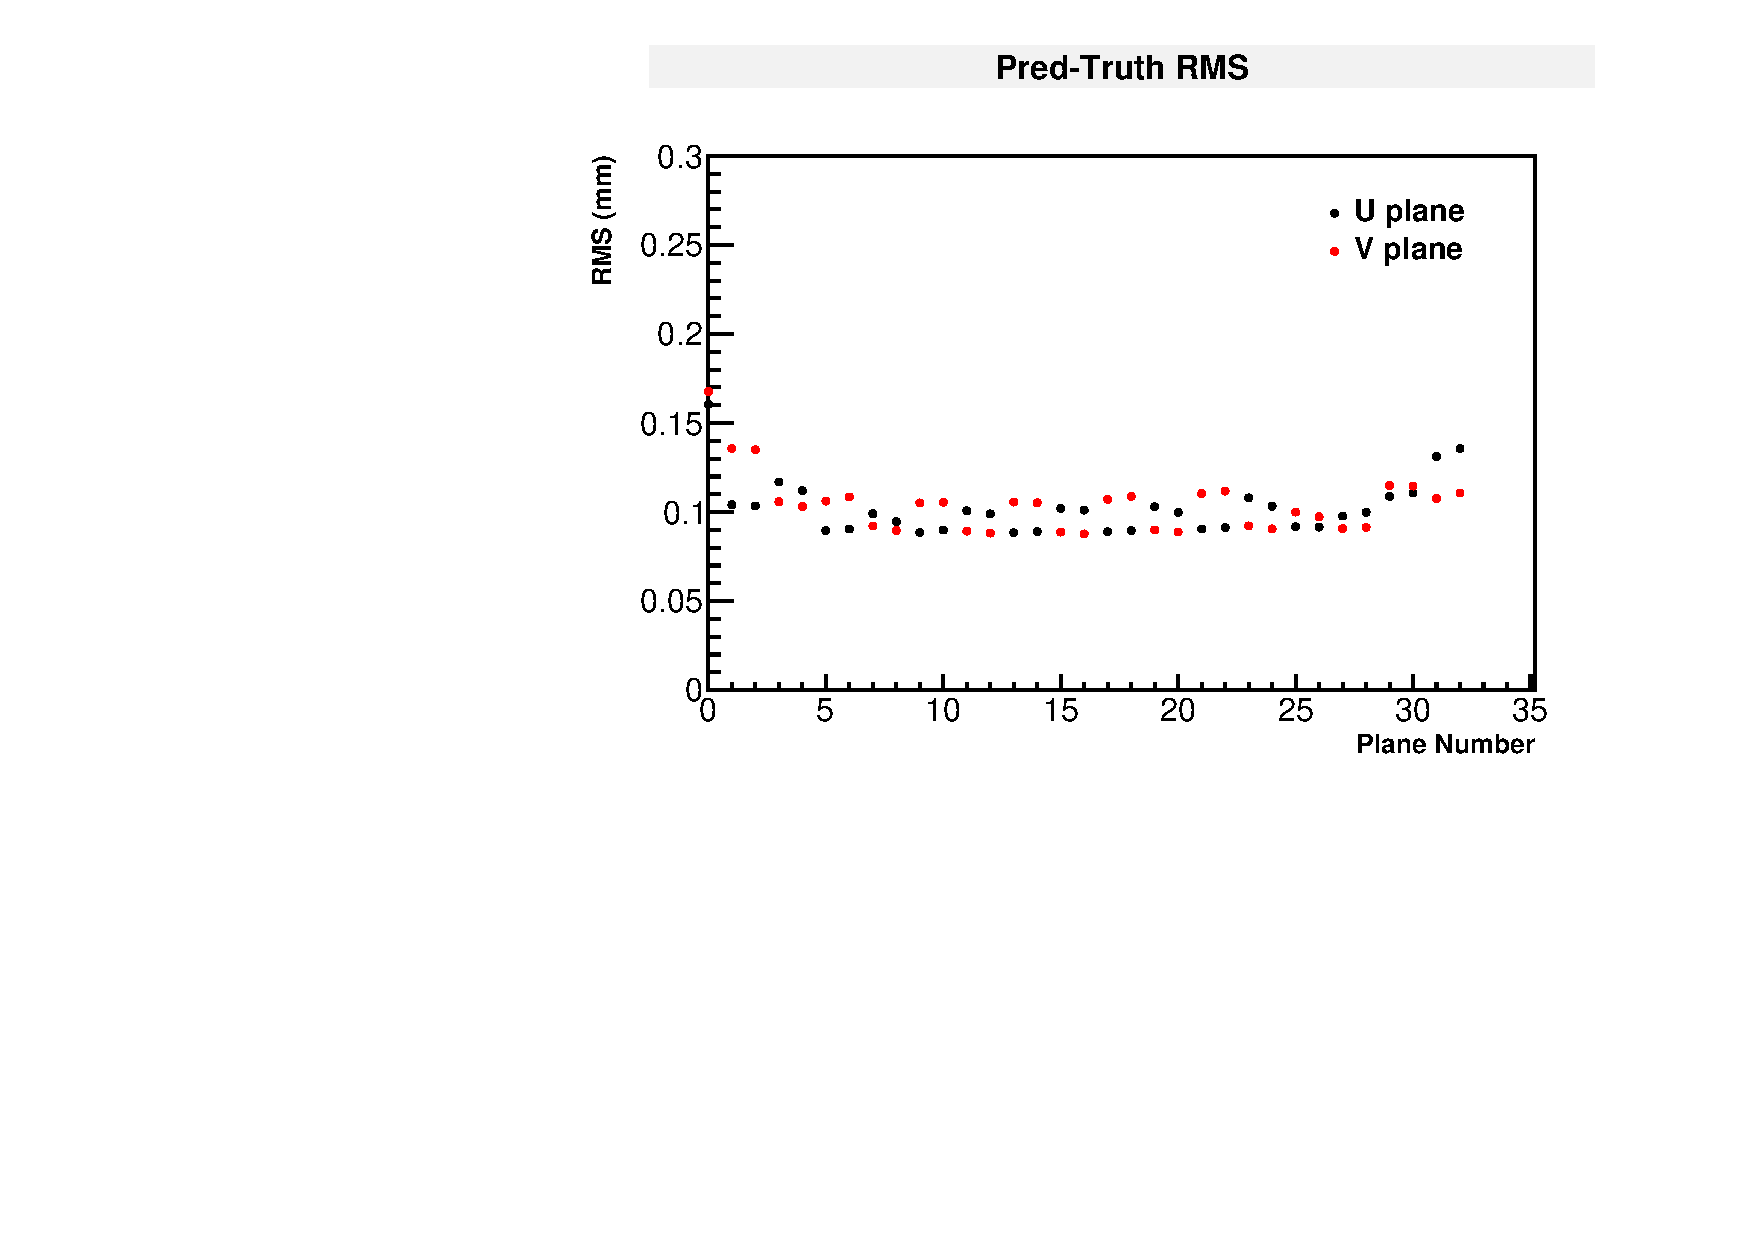
\includegraphics[width=1\textwidth]{predtruthrms} 
        \caption{RMS of predicted - truth residuals. There is an overall parabolic shape to the distribution, comprised of many parabolas. The RMS at the center of the fit is better than the edges since there are more measurements near the center. On individual planes, whatever that plane measured will have a better RMS, eg. plane 1 which is a U plane fits U better than V at that plane.}
    \end{subfigure}

    \caption{RMS of residual plots as a function of plane number for all events. Technically these should be split up according to number of planes hit, and the distance between the first and last hit in the fit, which would simplify and justify the shapes. See \href{http://gm2-docdb.fnal.gov:8080/cgi-bin/ShowDocument?docid=3813}{DocDB 3813} and \href{http://gm2-docdb.fnal.gov:8080/cgi-bin/ShowDocument?docid=6306}{DocDB 6306} to understand these plots.}
\end{figure}



\begin{figure}
    \centering
    \begin{subfigure}[]{0.6\textwidth}
        \centering
        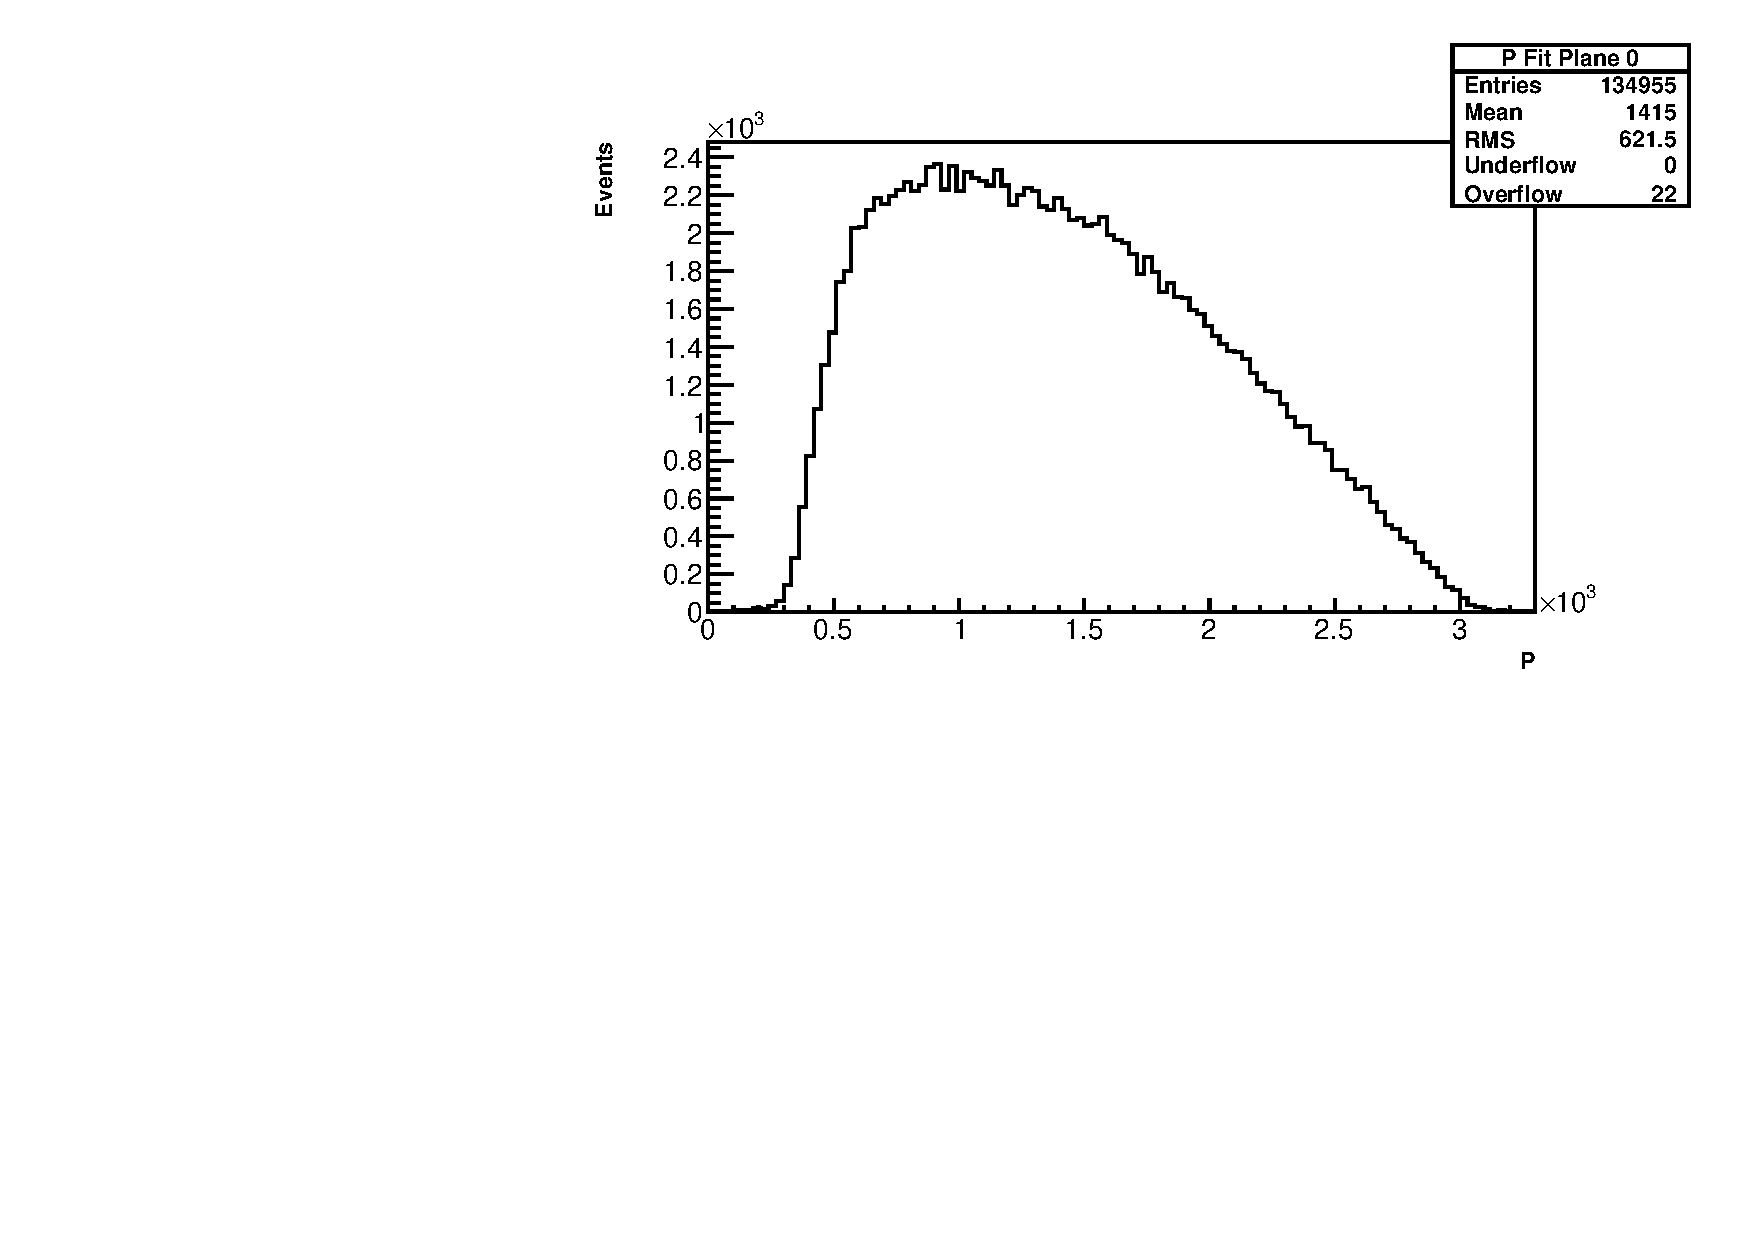
\includegraphics[width=1\textwidth]{Pplane0} 
        \caption{Momentum magnitude from the fit at plane 0. X momentum distribution is very similar to this since most of the momentum is in the forward direction.}
    \end{subfigure}

    \begin{subfigure}[]{0.6\textwidth}
        \centering
        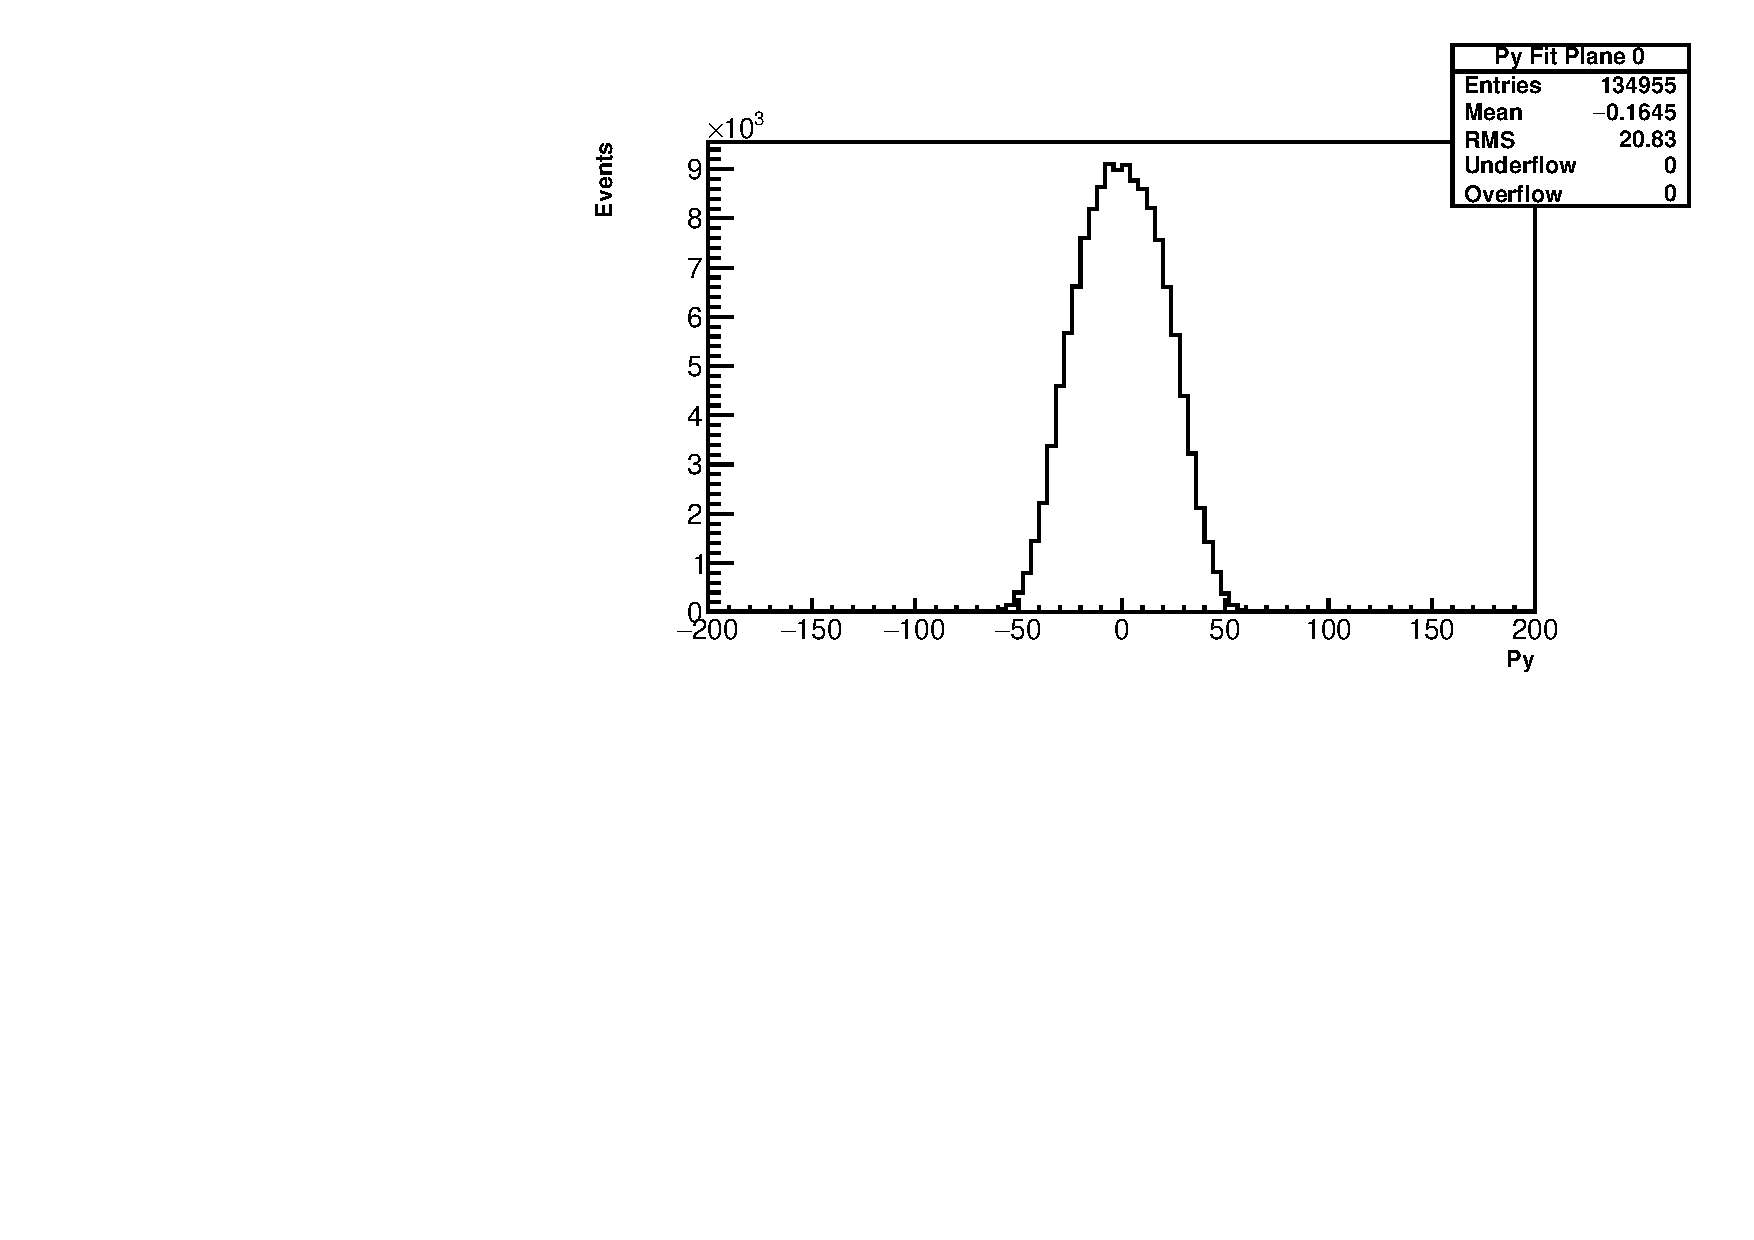
\includegraphics[width=1\textwidth]{Pyplane0} 
        \caption{Y momentum from the fit at plane 0. Bounded nicely by the measurement range of the detectors.}
    \end{subfigure}
    
    \begin{subfigure}[]{0.6\textwidth}
        \centering
        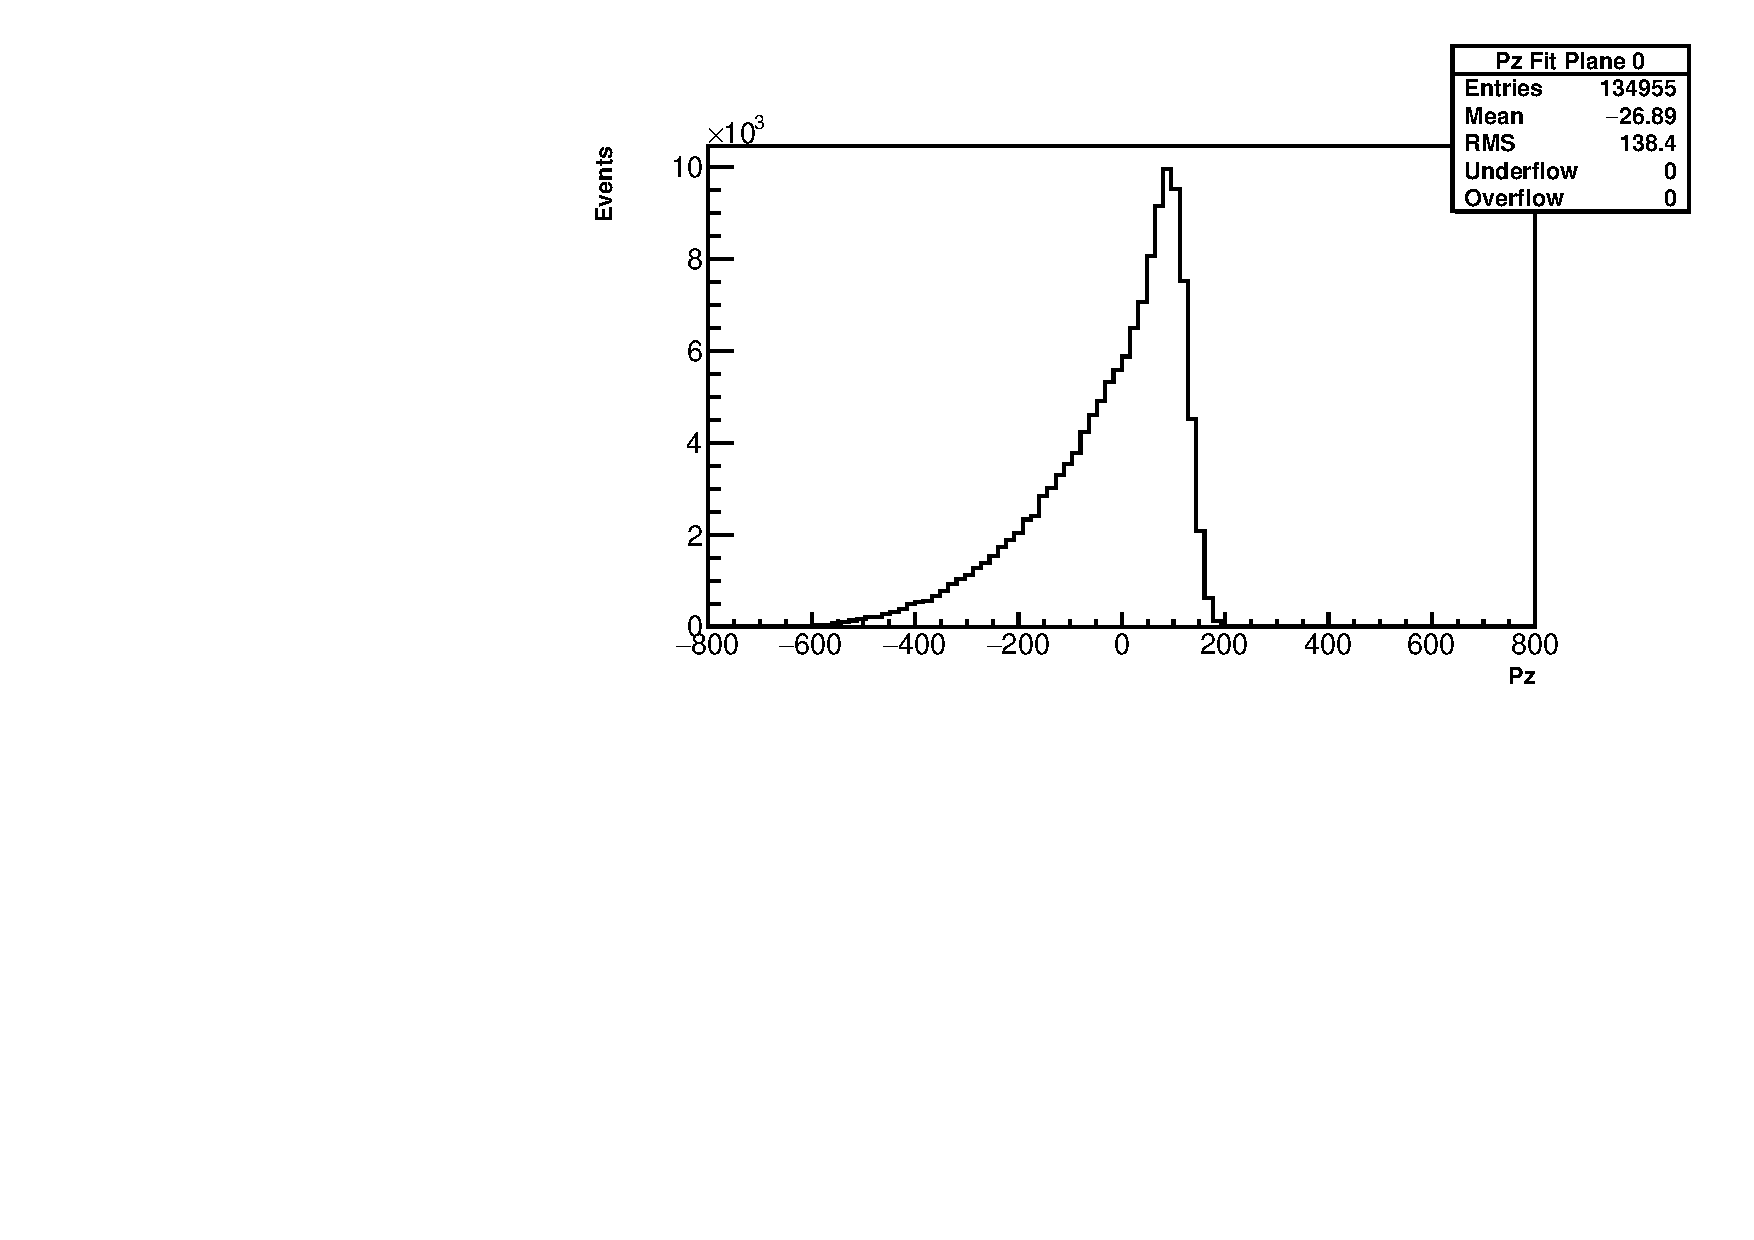
\includegraphics[width=1\textwidth]{Pzplane0} 
        \caption{Z momentum of the fit at plane 0. Some particles have outward radial momentum at the start of the fit (a negative value), and some inward, with all particles curving inward through the fit.}
    \end{subfigure}

    \caption{Momentum fit parameters on plane 0. Remember, the coordinate system is such that X is forward with the planes parallel, Y vertically up, and Z horizontal. The distributions here are very similar to truth as desired, which can be seen in the following truth residual plots.}
\end{figure}


\begin{figure}
    \centering
    \begin{subfigure}[]{0.55\textwidth}
        \centering
        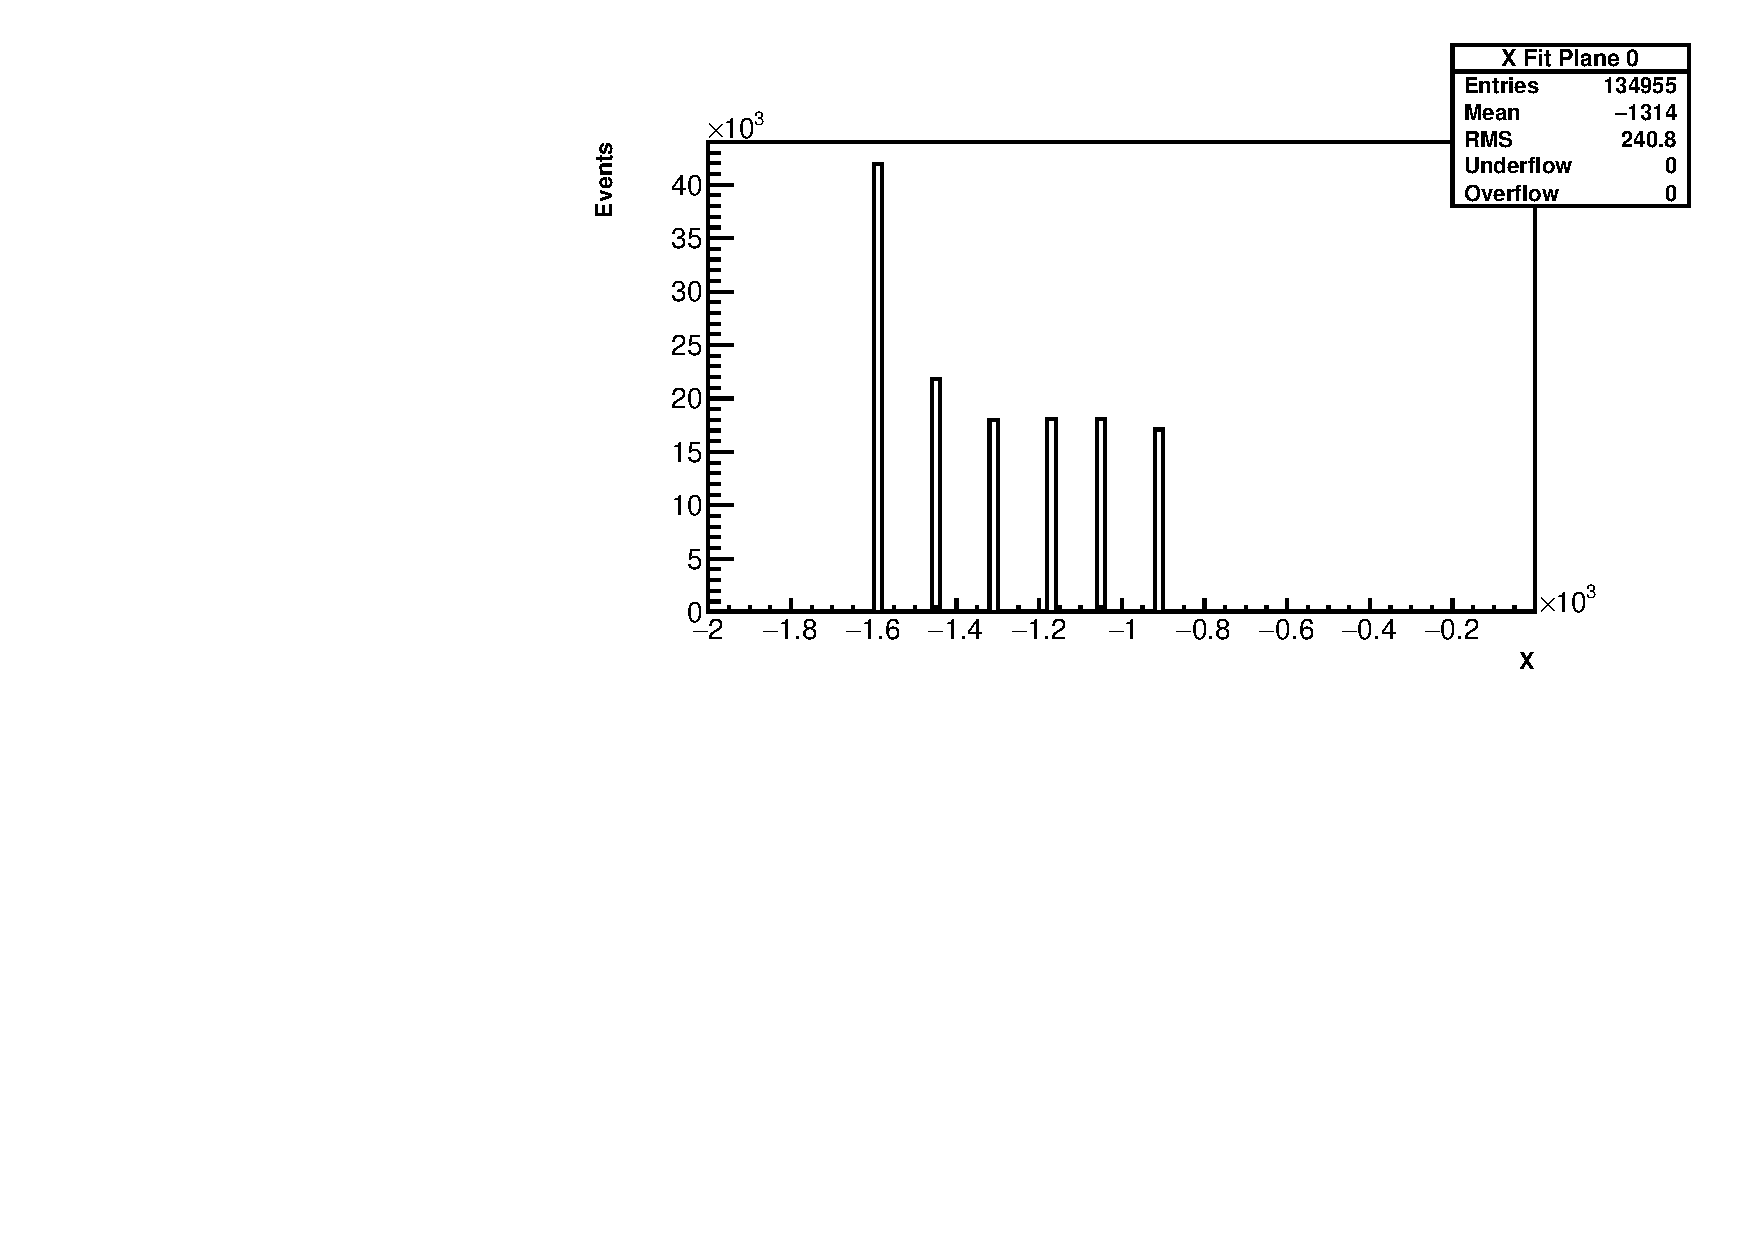
\includegraphics[width=1\textwidth]{Xplane0} 
        \caption{X position from the fit at plane 0. Made up of individual delta functions since fits start at discrete 0 planes before each module. No tracks with the current Geane fitting starts at module 7 or 8 since such tracks don't hit enough planes to be fit.}
    \end{subfigure}

    \begin{subfigure}[]{0.55\textwidth}
        \centering
        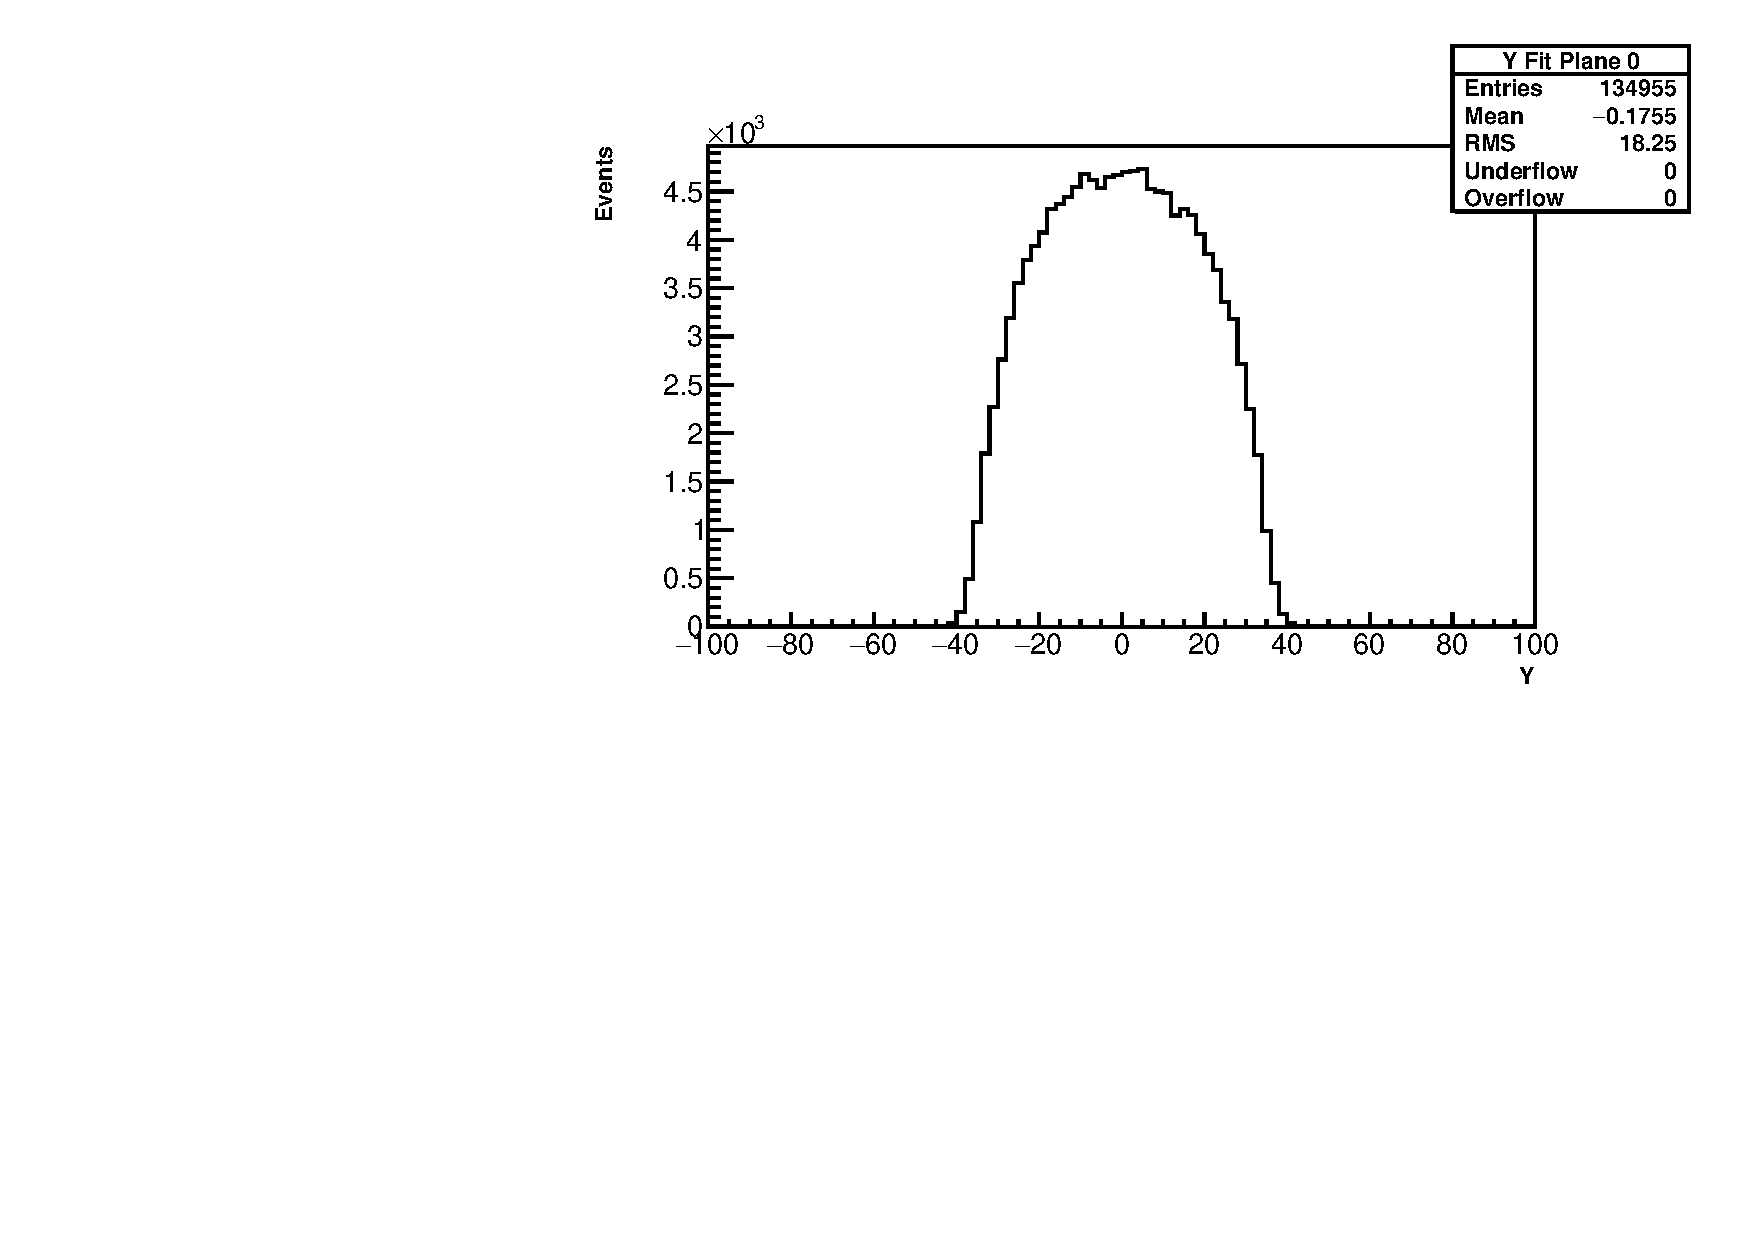
\includegraphics[width=1\textwidth]{Yplane0} 
        \caption{Y position from the fit at plane 0. Bounded nicely by the measurement range of the detectors. The storage region width can be seen.}
    \end{subfigure}
    
    \begin{subfigure}[]{0.55\textwidth}
        \centering
        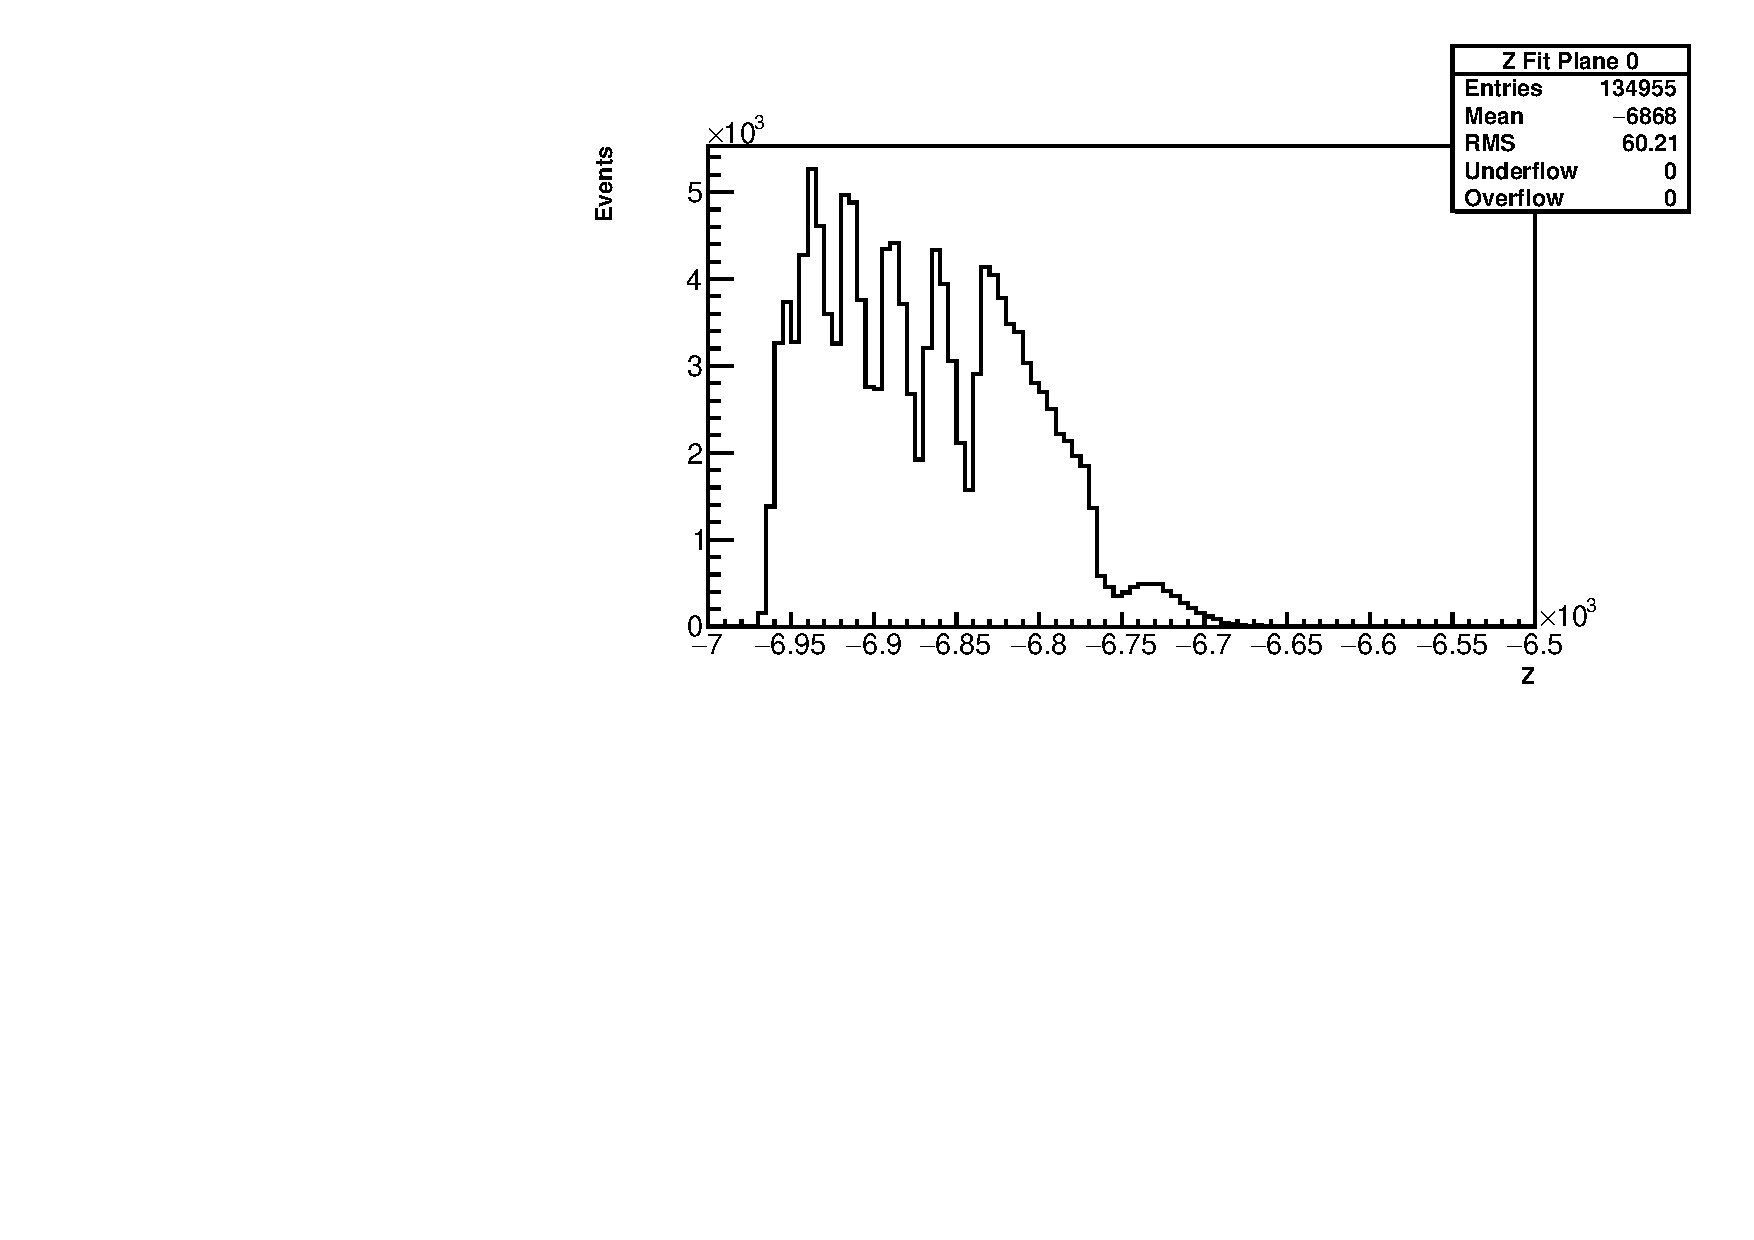
\includegraphics[width=1\textwidth]{Zplane0} 
        \caption{Z position of the fit at plane 0. There is an interesting spiky structure to the distribution, coming from how the detectors are staggered and shifted, and the incoming distribution of positrons. A larger negative value indicates a greater radial position. As a reminder this distribution is seen in truth as well.}
    \end{subfigure}

    \caption{Position fit parameters on plane 0. Remember, the coordinate system is such that X is forward with the planes parallel, Y vertically up, and Z horizontal. The distributions here are very similar to truth as desired, which can be seen in the following truth residual plots.}
\end{figure}


\begin{figure}
    \centering
    \begin{subfigure}[]{0.6\textwidth}
        \centering
        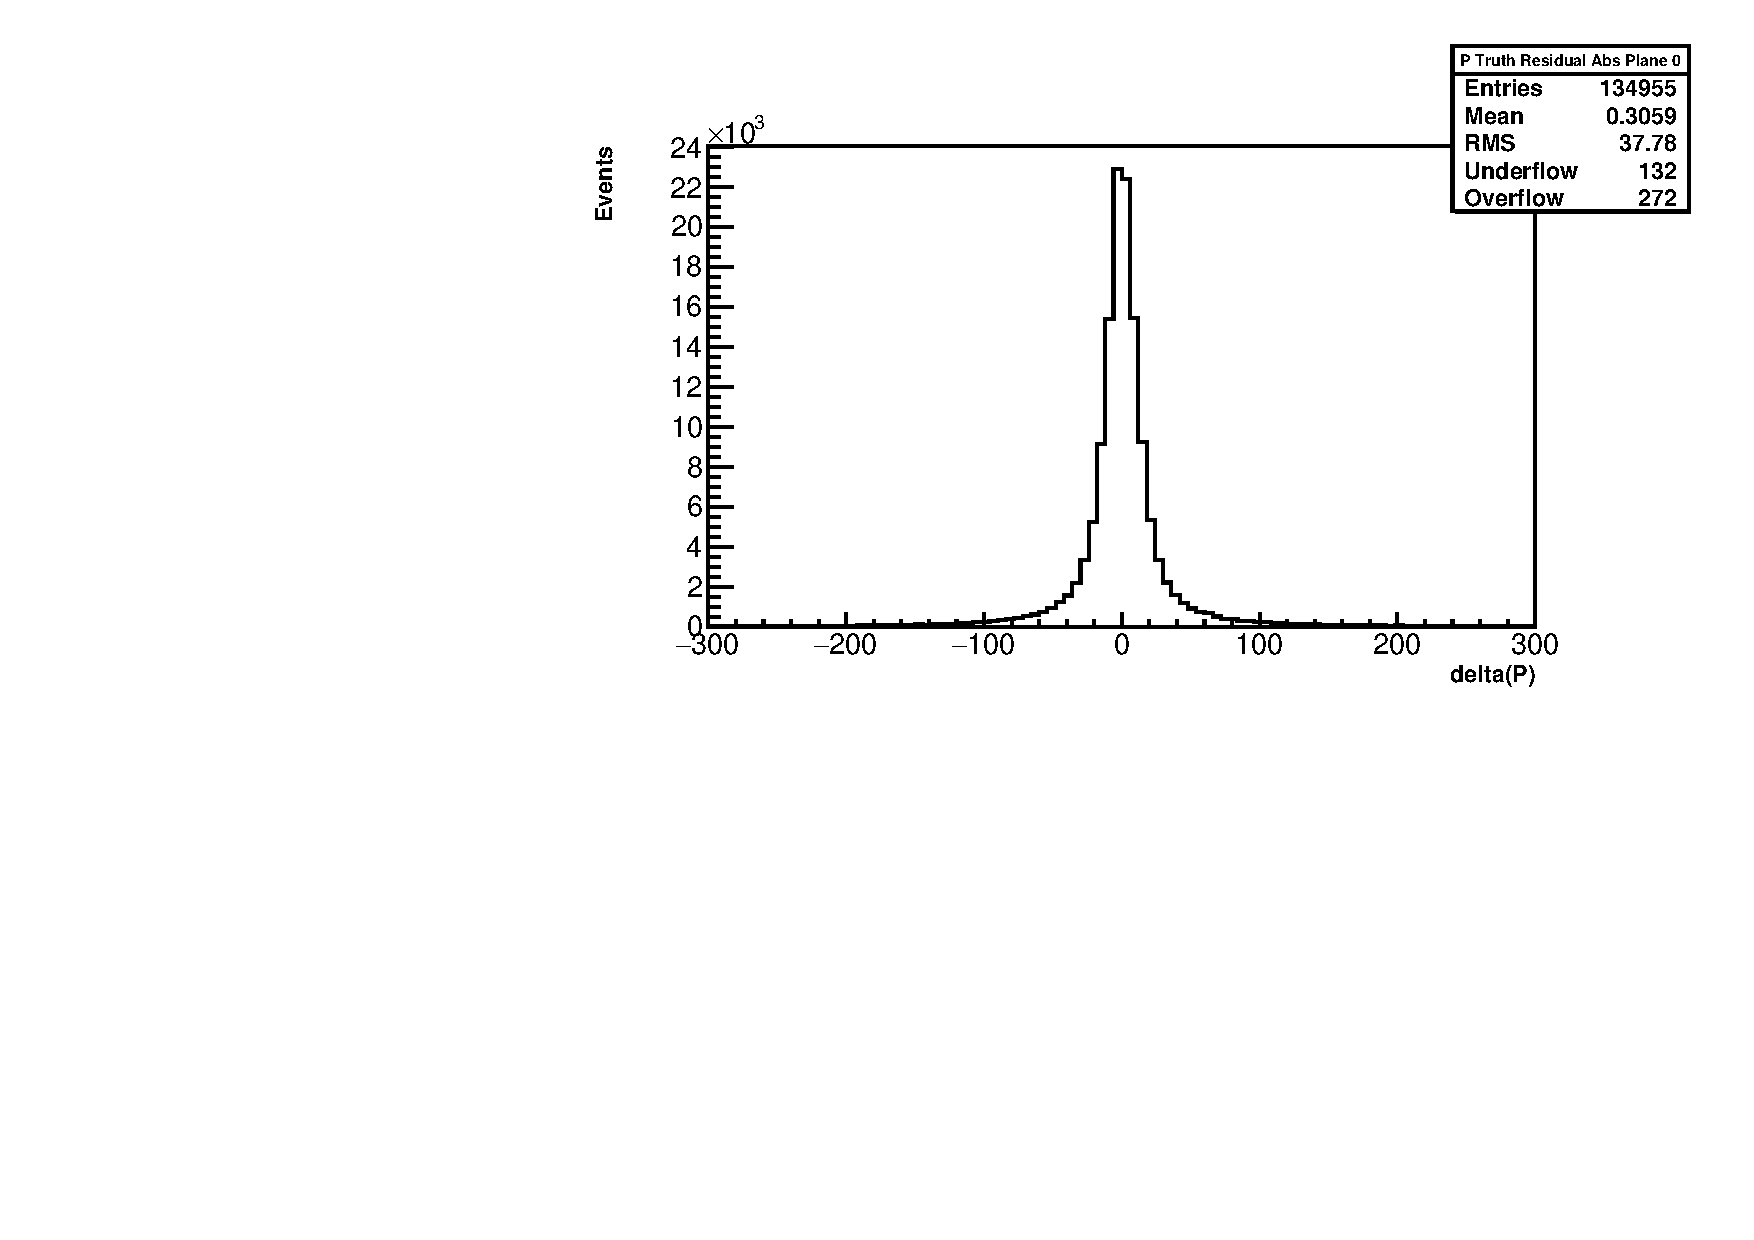
\includegraphics[width=1\textwidth]{P0TruthRes} 
        \caption{Momentum truth residual on plane 0. The distribution has an RMS of about 40 MeV.}
    \end{subfigure}

    \begin{subfigure}[]{0.6\textwidth}
        \centering
        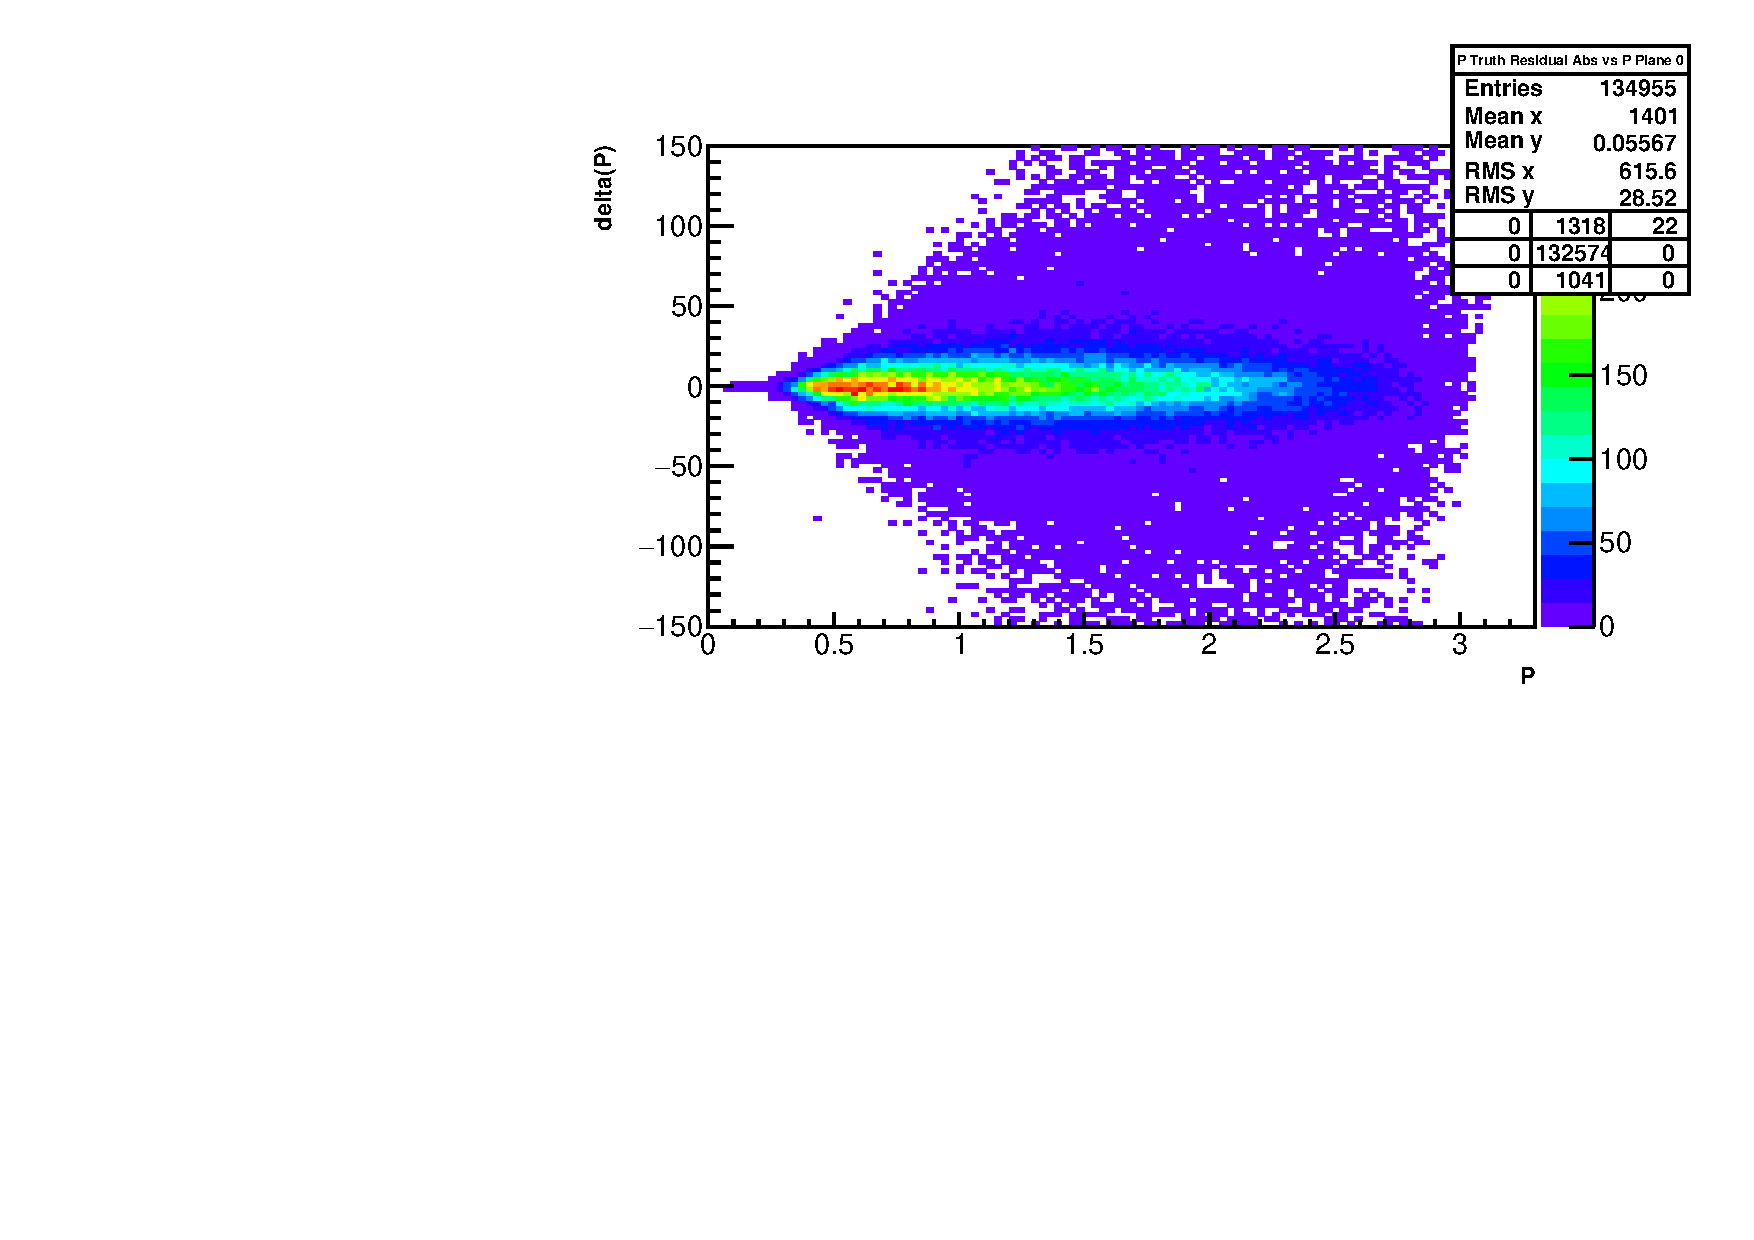
\includegraphics[width=1\textwidth]{P0TruthResVsP} 
        \caption{Momentum truth residual on plane 0 vs P. As the momentum increase the spread in the residual increases, with the core staying relatively tight.}
    \end{subfigure}
    
    \begin{subfigure}[]{0.6\textwidth}
        \centering
        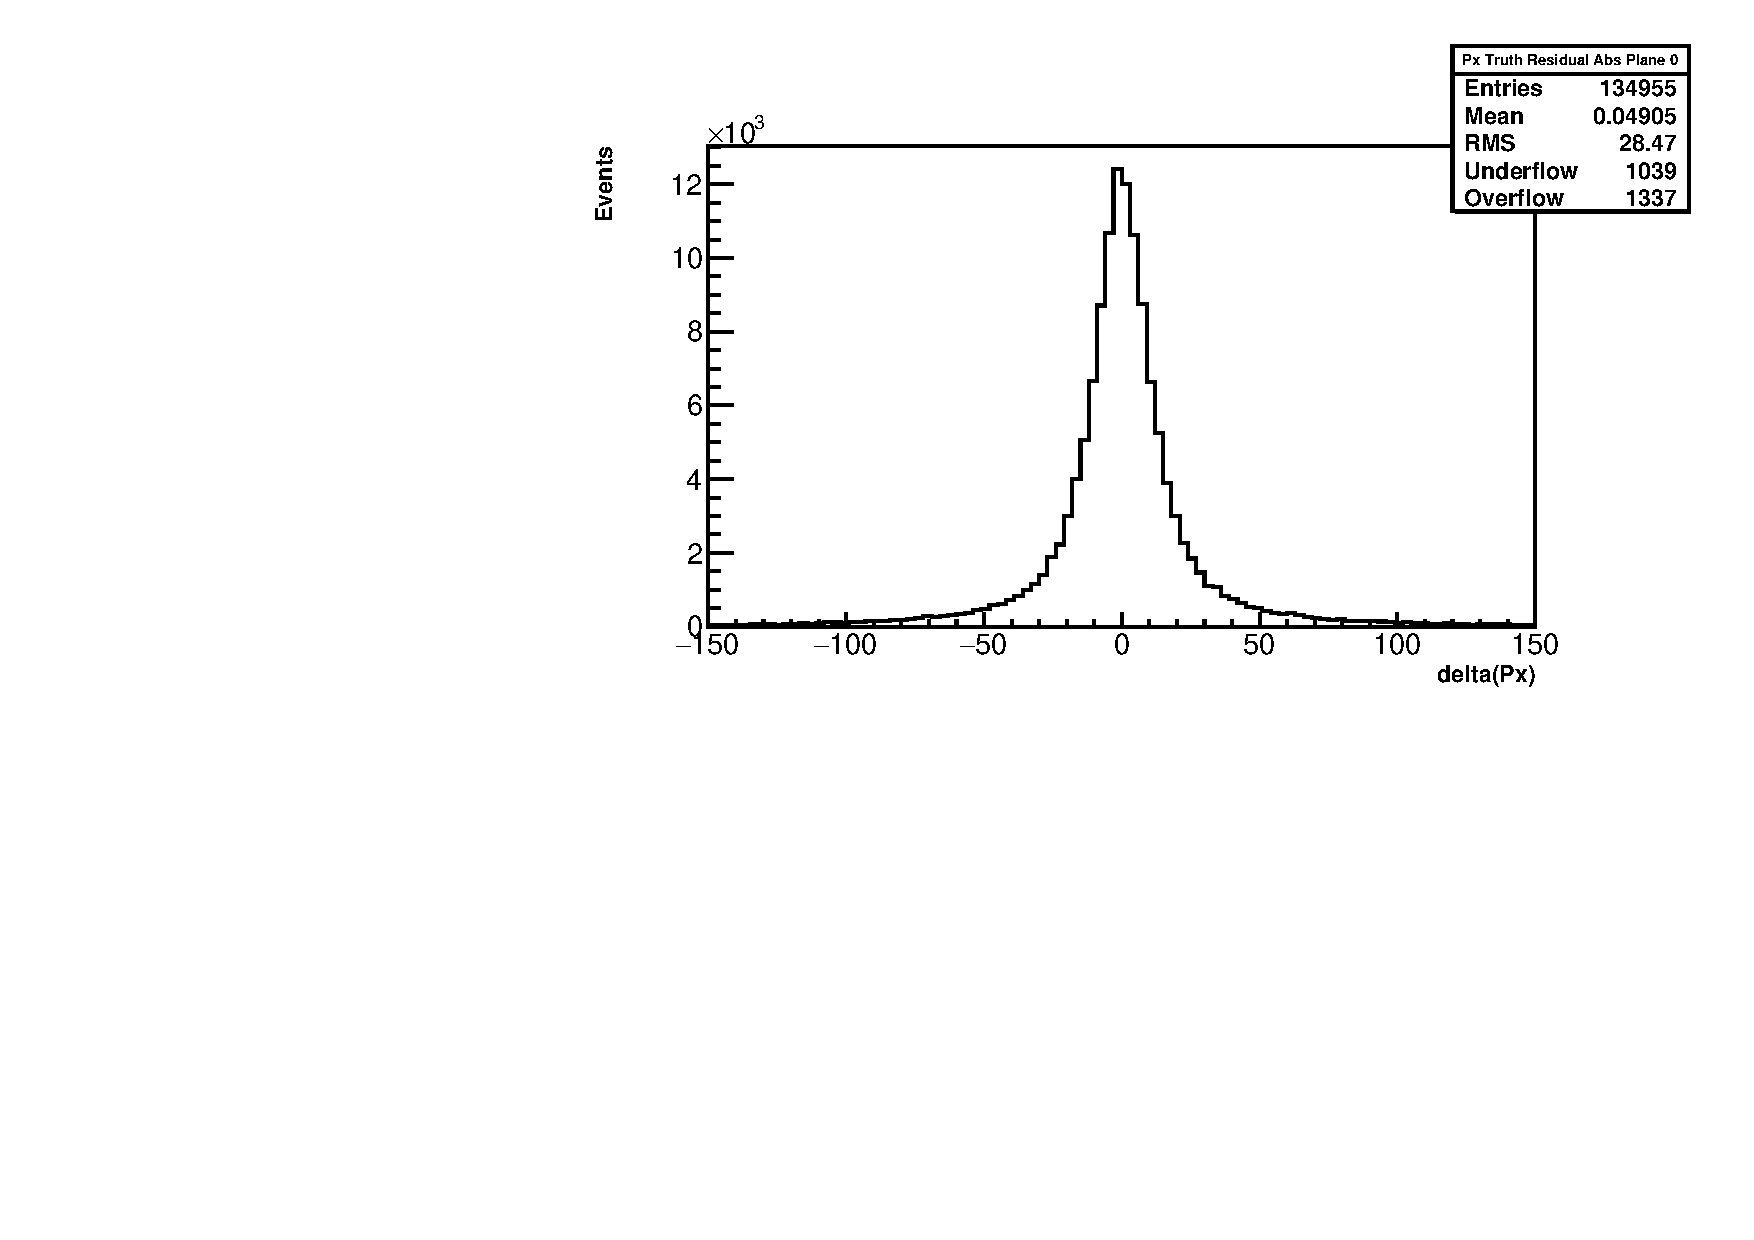
\includegraphics[width=1\textwidth]{Px0TruthRes} 
        \caption{X momentum truth residual on plane 0. Has an RMS of about 30 MeV. There are large tails in the distribution.}
    \end{subfigure}

    \caption{Momentum truth residuals on plane 0. Units are MeV. Most of the momentum and momentum spread is in the forward X direction. For real examination all of these plots should be split up according to the momentum of the track.}
\end{figure}


\begin{figure}
    \centering
    \begin{subfigure}[]{0.6\textwidth}
        \centering
        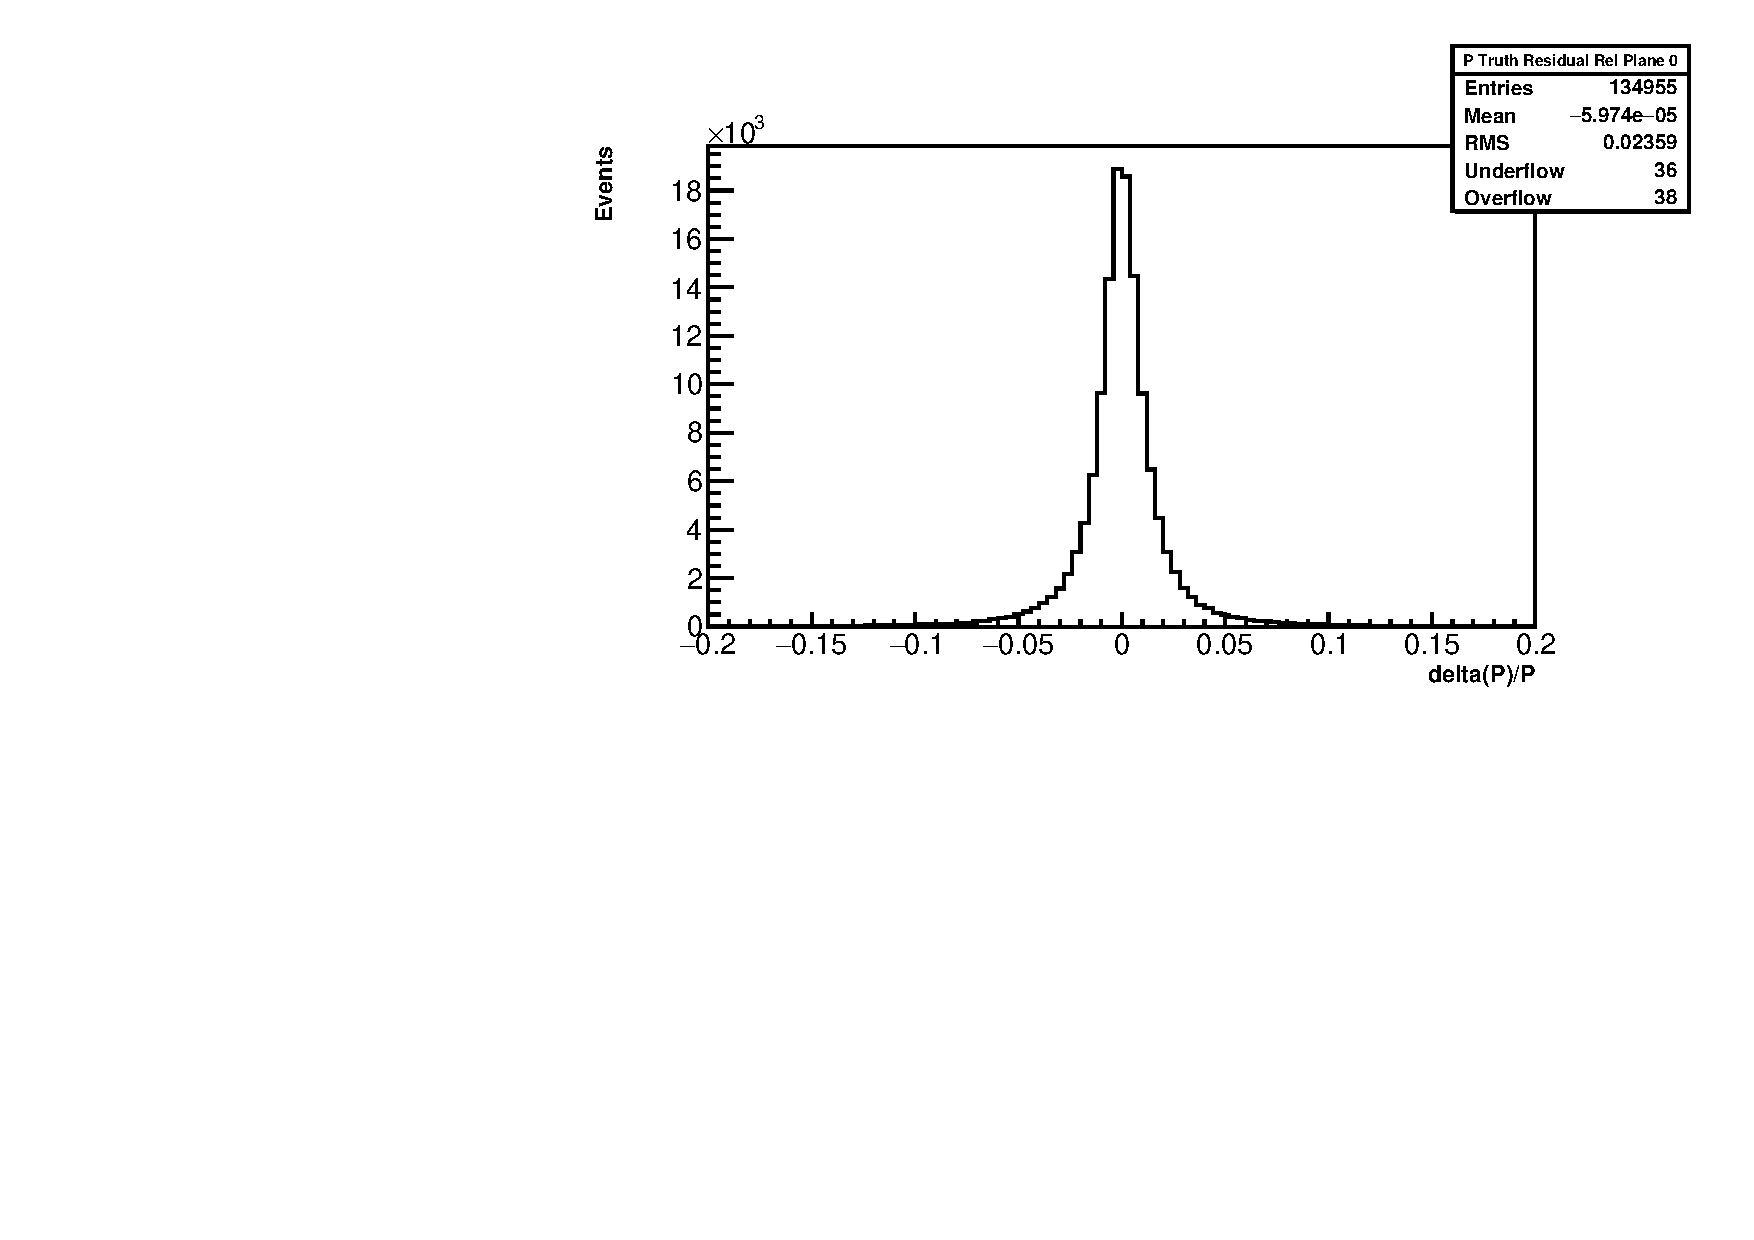
\includegraphics[width=1\textwidth]{P0TruthResRel} 
        \caption{Relative momentum truth residual on plane 0. There is about a 2\% resolution to the track fitting.}
    \end{subfigure}

    \begin{subfigure}[]{0.6\textwidth}
        \centering
        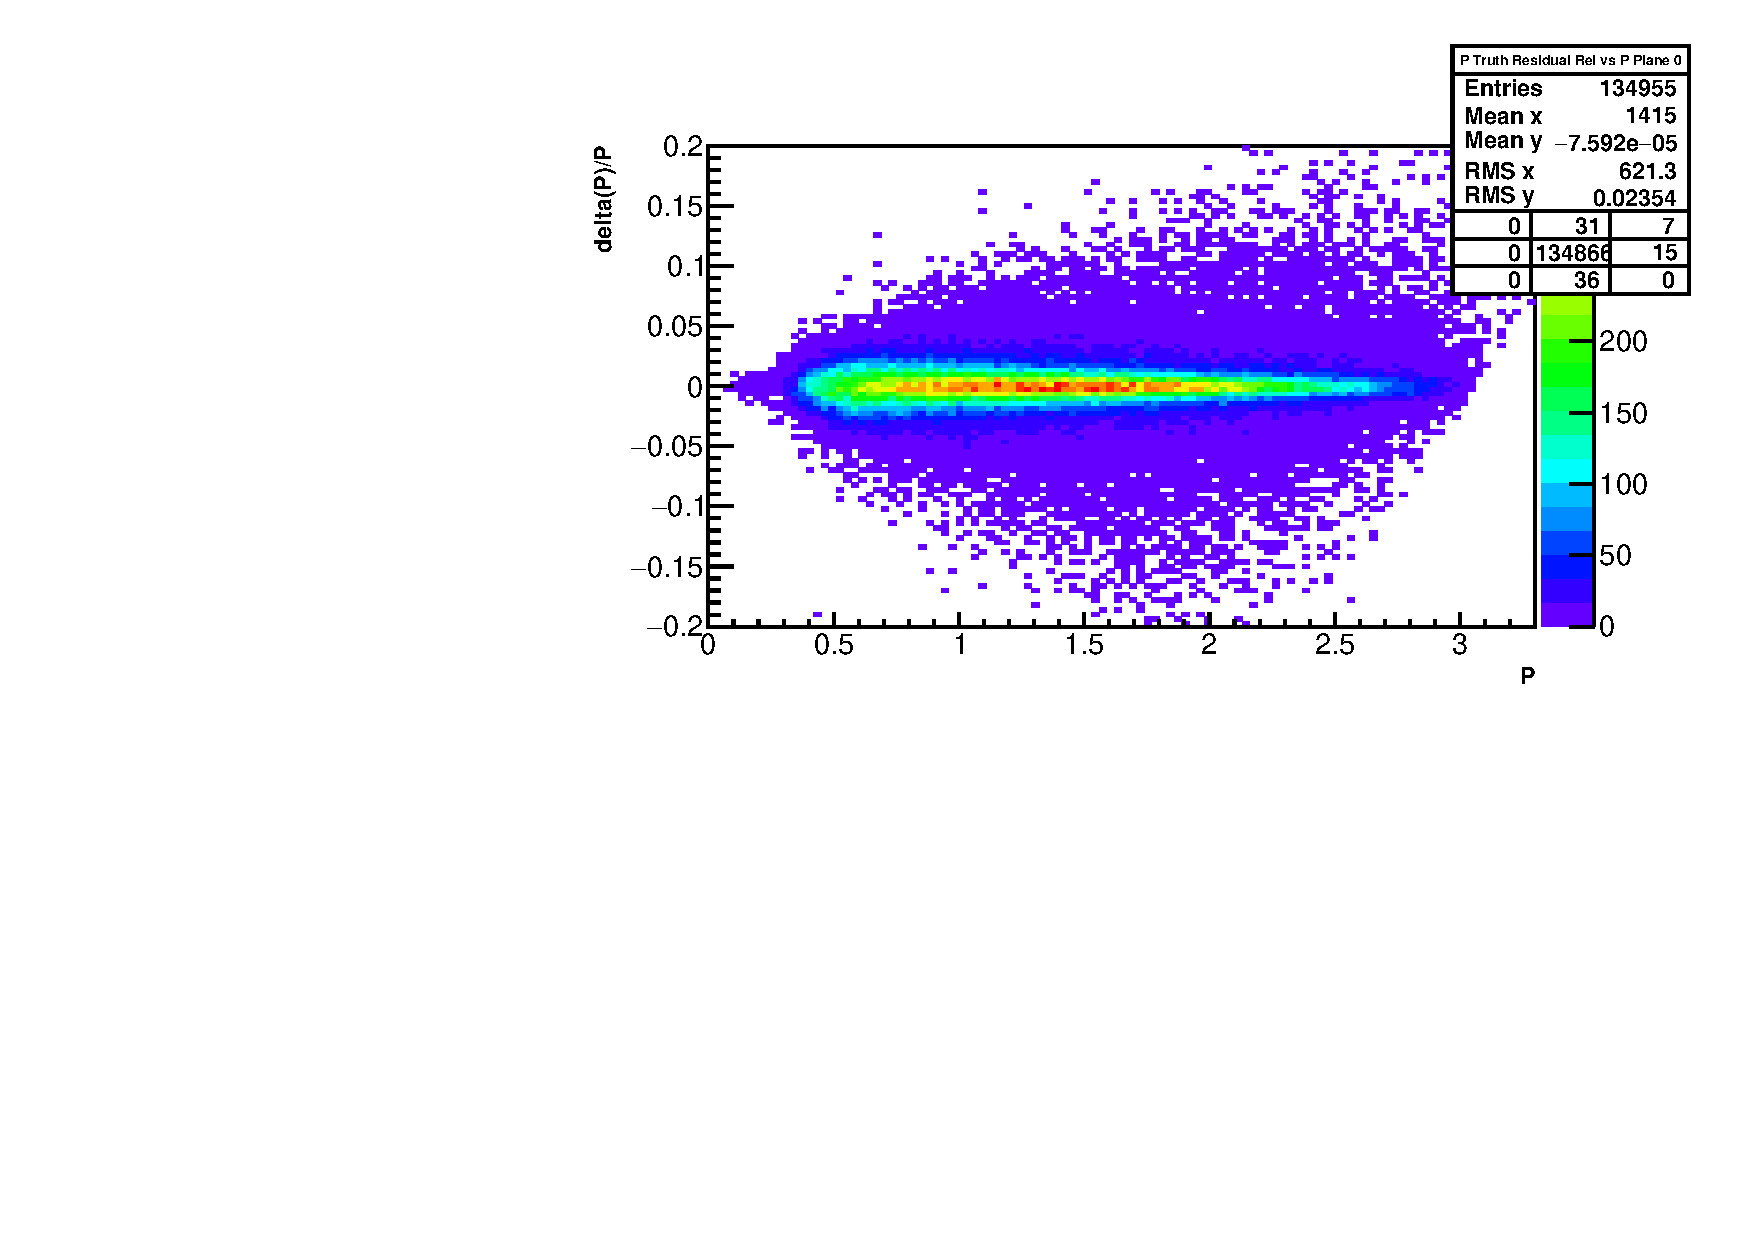
\includegraphics[width=1\textwidth]{P0TruthResVsPRel} 
        \caption{Relative momentum truth residual on plane 0 vs P. There is a tendency of the track fitting to overestimate the momentum of the track for some high momentum tracks.}
    \end{subfigure}
    
    \begin{subfigure}[]{0.6\textwidth}
        \centering
        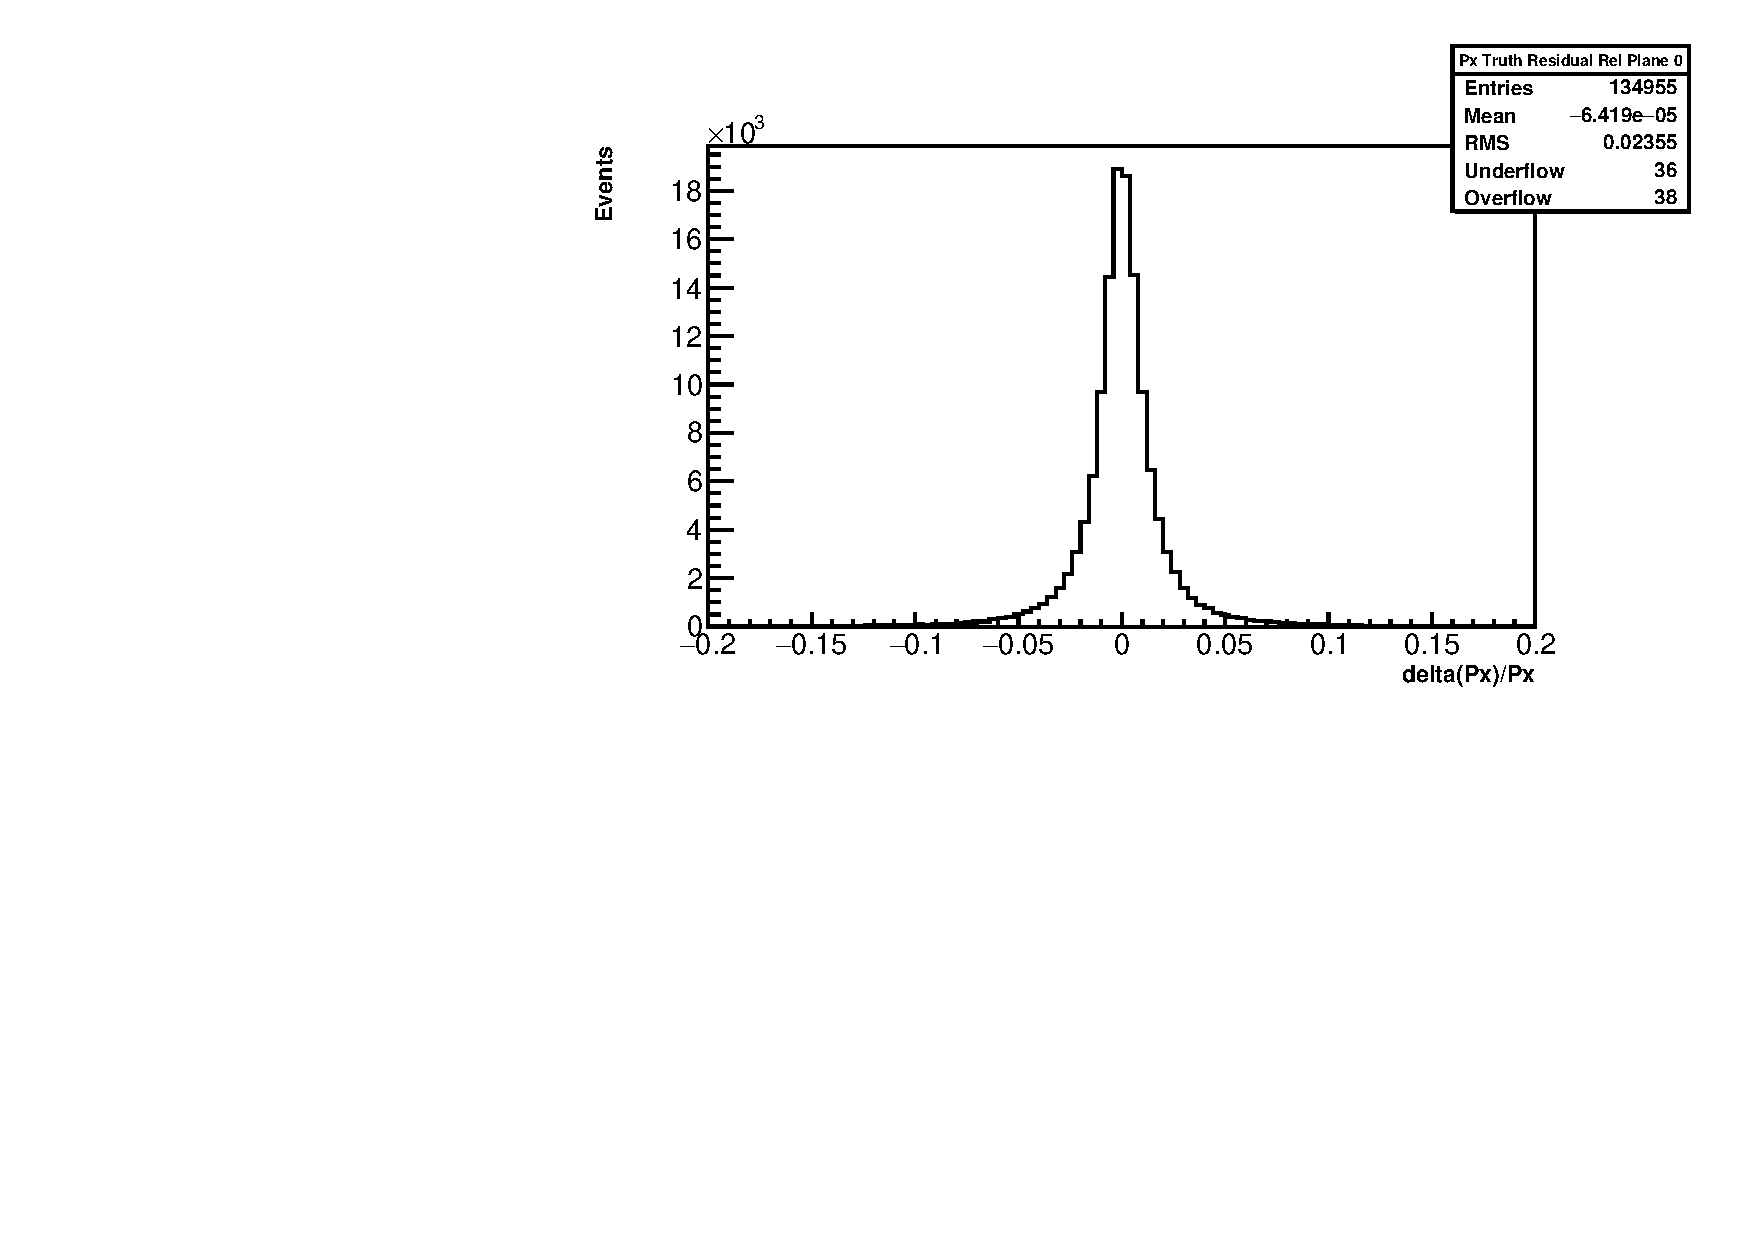
\includegraphics[width=1\textwidth]{Px0TruthResRel} 
        \caption{X relative momentum truth residual on plane 0.}
    \end{subfigure}

    \caption{Relative momentum truth residuals on plane 0. For real examination all of these plots should be split up according to the momentum of the track.}
\end{figure}



\begin{figure}
    \centering
    \begin{subfigure}[]{0.6\textwidth}
        \centering
        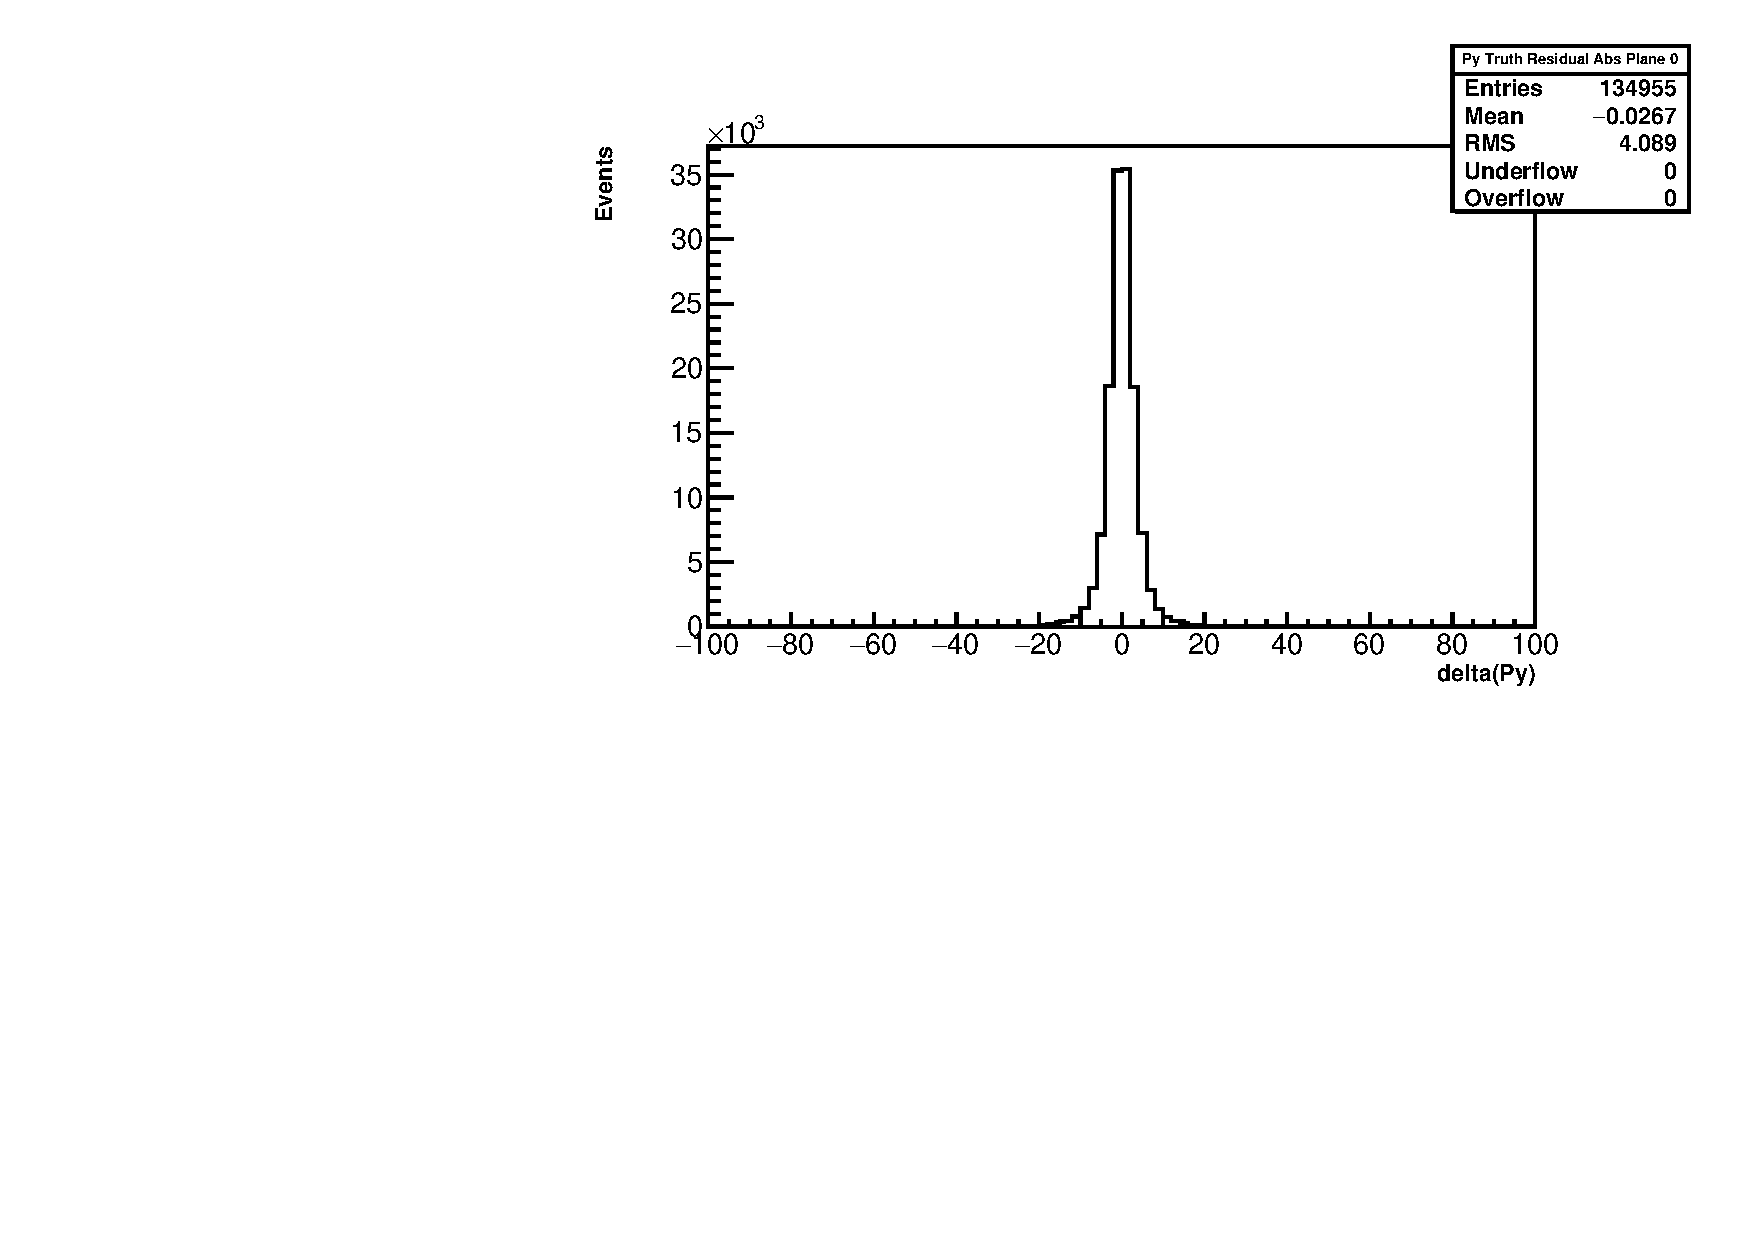
\includegraphics[width=1\textwidth]{Py0TruthRes} 
        \caption{Y momentum truth residual on plane 0. The distribution has an RMS of about 4 MeV indicating the vertical momentum is pretty well measured, though tracks generally do not have much vertical momentum.}
    \end{subfigure}

    \begin{subfigure}[]{0.6\textwidth}
        \centering
        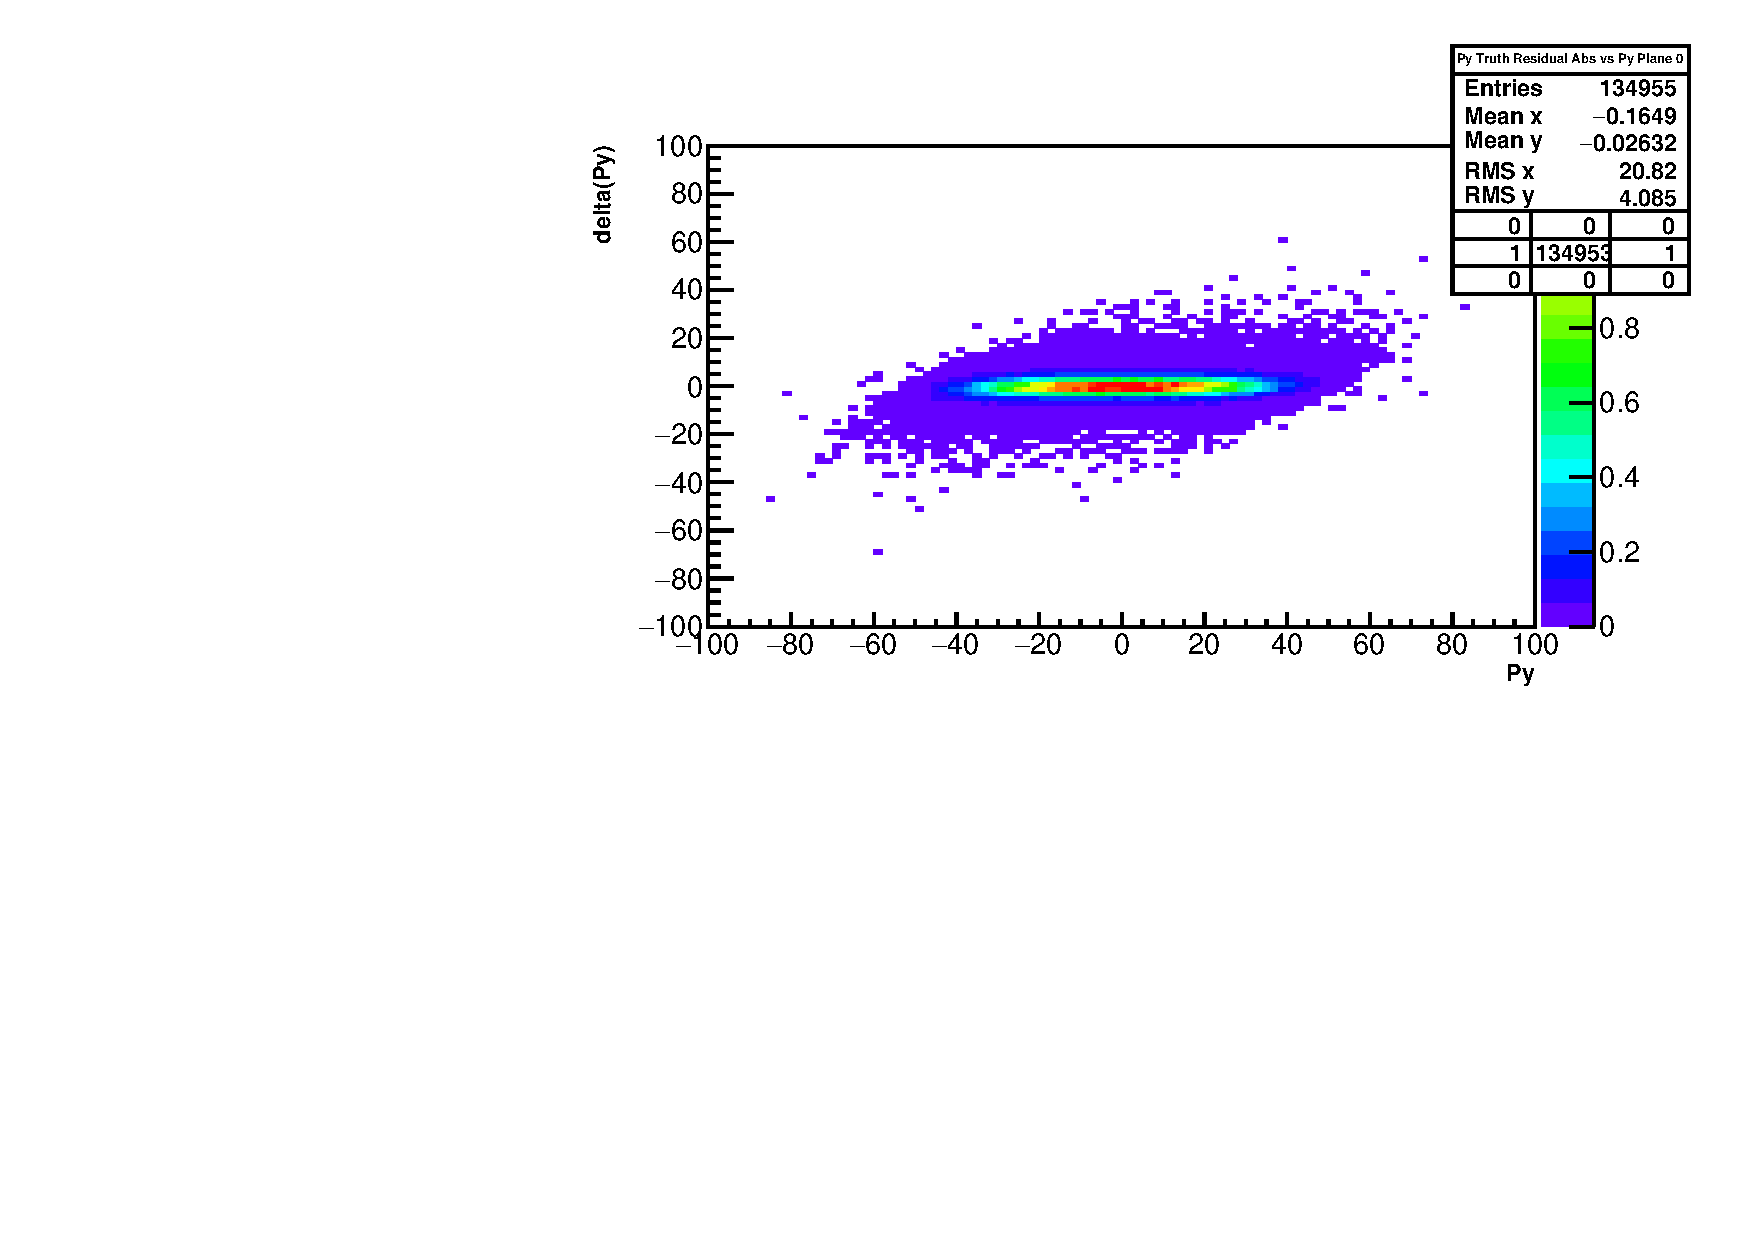
\includegraphics[width=1\textwidth]{Py0TruthResVsP} 
        \caption{Y momentum truth residual on plane 0 vs Py. There is a pretty tight core and some small corners in the distribution.}
    \end{subfigure}
    
    \begin{subfigure}[]{0.6\textwidth}
        \centering
        \includegraphics[width=1\textwidth]{Pz0TruthRes} 
        \caption{Z momentum truth residual on plane 0. Has an RMS of about 3 MeV, indicating the horizontal momentum is pretty well measured, though tracks generally do not have much horizontal momentum.}
    \end{subfigure}

    \caption{Momentum truth residuals on plane 0. Units are MeV. For real examination all of these plots should be split up according to the momentum of the track.}
\end{figure}

\clearpage

\begin{figure}
    \centering
    \begin{subfigure}[]{0.6\textwidth}
        \centering
        \includegraphics[width=1\textwidth]{X0TruthRes} 
        \caption{X position truth residual on plane 0. The distribution is a spike indicating that the X position of the fit is taken as known when fitting. Non-zero values indicate something is wrong with the fitting.}
    \end{subfigure}

    \begin{subfigure}[]{0.6\textwidth}
        \centering
        \includegraphics[width=1\textwidth]{Y0TruthRes} 
        \caption{Y position truth residual on plane 0. Has an RMS of about 740 $\mu$m as expected from simple geometry arguments coming from the 150 $\mu$m smearing. Even though particles do not curve much in Y, the straws don't measure the vertical position very well.}
    \end{subfigure}
    
    \begin{subfigure}[]{0.6\textwidth}
        \centering
        \includegraphics[width=1\textwidth]{Z0TruthRes} 
        \caption{Z position truth residual on plane 0. Has an RMS of about 135 $\mu$m as expected from simple geometry arguments coming from the 150 $\mu$m smearing. Better than the Y residual since both straws measure mostly in the horizontal direction, in spite of the fit having to deal with the curvature of the tracks.}
    \end{subfigure}

    \caption{Position truth residuals on plane 0. Units are mm. For real examination all of these plots should be split up according to the momentum of the track.}
\end{figure}




